%%%%%%%%%%%%%%%%%%%%%%%%%%%%%%%%%%%%%%%%%%%%%%%%
%
% Strath PhD Thesis Template
%  by Jethro Browell [jethro.browell@strath.ac.uk]
%
%  Guidelines for thesis format, submission and content are found in
%  General and Course Regulations for Graduate and Postgraduate
%  Awards and Degrees, section 20.6.
%
%  Using .eps or .pdf is recomended to prduce high quality figures etc.
%
%  The Strathclyde logo can be found in other formats at www.strath.ac.uk.
%
%%%%%%%%%%%%%%%%%%%%%%%%%%%%%%%%%%%%%%%%%%%%%%%%

\documentclass[a4paper,oneside,11pt]{book}

%\includeonly{simple}

\usepackage{amsbsy}
\usepackage{amsmath}
\usepackage{amsfonts}
\usepackage{graphicx}
\usepackage{multirow}
\usepackage{mathrsfs}
\usepackage{xcolor}
\usepackage[hidelinks]{hyperref}
\usepackage{cite}
\usepackage{enumitem}
\usepackage{epsfig}
\usepackage{caption}
\usepackage{subcaption}
\usepackage[strict]{changepage}

\usepackage{amssymb}
\usepackage{amsthm}
\usepackage{catchfilebetweentags}
\usepackage[capitalize]{cleveref}
\usepackage{cmll}
\usepackage{ebproof}
\usepackage[utf8]{inputenc}
\usepackage{mathtools}
\usepackage{mathpartir}
\usepackage{multicol}
\usepackage[numbers]{natbib}
\usepackage{newunicodechar}
\usepackage{rotating}
\usepackage{stmaryrd}
\usepackage{todonotes}
\usepackage{turnstile}

\usepackage{tikz}
\usetikzlibrary{cd,fit,matrix,positioning}

\usepackage[conor]{agda}

\theoremstyle{definition}
\newtheorem{theorem}{Theorem}[section]
\newtheorem{conjecture}[theorem]{Conjecture}
\newtheorem{proposition}[theorem]{Proposition}
\newtheorem{lemma}[theorem]{Lemma}
\newtheorem{corollary}[theorem]{Corollary}
\newtheorem{example}[theorem]{Example}
\newtheorem{definition}[theorem]{Definition}
\newtheorem{remark}[theorem]{Remark}

\definecolor{use}{HTML}{008000}
\newcommand\gr[1]{{\color{use}#1}}
\newcommand\grctx[1]{\gr{\mathcal{#1}}}
\newcommand\grP{\grctx P}
\newcommand\grQ{\grctx Q}
\newcommand\grR{\grctx R}
\newcommand\grPprime{\grP\gr'}
\newcommand\grQprime{\grQ\gr'}
\newcommand\grRprime{\grR\gr'}
\newcommand\name{\ensuremath{\lambda\grR}}
\newcommand\grctxsub[2]{\grctx{#1}_{\gr{#2}}}
\newcommand\grPe{\grctxsub P e}
\newcommand\grPf{\grctxsub P f}
\newcommand\grPl{\grctxsub P l}
\newcommand\grPr{\grctxsub P r}
\newcommand\grQe{\grctxsub Q e}
\newcommand\grQf{\grctxsub Q f}
\newcommand\grQl{\grctxsub Q l}
\newcommand\grQr{\grctxsub Q r}
\newcommand\grRl{\grctxsub R l}
\newcommand\grRr{\grctxsub R r}
\newcommand\ps{\mathit{ps}}
\newcommand\qs{\mathit{qs}}
\newcommand\rs{\mathit{rs}}
\newcommand\dotto{\mathrel{\dot\to}}
\newcommand\dotlr{\mathrel{\dot\leftrightarrow}}
\newcommand\dottimes{\mathbin{\dot\times}}
%\newcommand\dotplus{\mathbin{\dot+}}
\newcommand\wand{\mathrel{\mathord{-}\hspace{-0.75ex}*}}
\newcommand\sep{\mathbin{*}}
\newcommand\Boxzp{\Box^{0{+}}}
\newcommand\Boxzpt{\Box^{0{+}{*}}}
\providecommand\U{}
\renewcommand\U{\mathcal U}
\newcommand\V{\mathcal V}
\newcommand\W{\mathcal W}
\providecommand\C{}
\renewcommand\C{\mathcal C}
\newcommand\sqin{\mathrel{\mathrlap{\sqsubset}{\mathord{-}}}}
\newcommand\sqni{\mathrel{\mathrlap{\sqsupset}{\mathord{-}}}}
\newcommand\Ann{\mathscr R}

\renewcommand\land{~\wedge~}
\renewcommand\lor{~\vee~}
\newcommand\rel{\mathrel{\mathord{\to}\hspace{-2.25ex}+}}

\DeclareMathOperator\Set{Set}
\DeclareMathOperator\obj{Obj}
\DeclareMathOperator\List{List}
\let\hom\relax
\DeclareMathOperator\hom{Hom}
\DeclareMathOperator\id{id}
\DeclareMathOperator\sub{Sub}

\newcommand\env[1]{\stackrel{#1}\Longrightarrow}

\usepackage{mleftright}
\newcommand\lr[3]{\mleft#1{#2}\mright#3}
\newcommand\sem[1]{\lr\llbracket{#1}\rrbracket}
\newcommand\size[1]{\lr\lvert{#1}\rvert}
\newcommand\plr[1]{\lr({#1})}
\newcommand\blr[1]{\lr[{#1}]}
\newcommand\forallb[1]{\forall\blr{~#1~}}
\newcommand\alr[1]{\lr\langle{#1}\rangle}
\newcommand\bra[1]{\lr\langle{#1}\rvert}
\newcommand\ket[1]{\lr\lvert{#1}\rangle}

\newcommand\leO{\;{\leq}0}
\newcommand\leI{\;{\leq}1}

\DeclareMathOperator{\lin}{lin}
\DeclareMathOperator{\intu}{int}
\newcommand\lnl{\ensuremath{\mathrm{L/nL}}}
\newcommand\vdashL{\mathrel{\vdash_{\mathcal L}}}
\newcommand\vdashC{\mathrel{\vdash_{\mathcal C}}}

\ebproofnewstyle{comb}{separation=0.75em}
\ebproofset{right label template=\TirName{\inserttext}}

\newenvironment{eqns}{\begin{array}{r@{\hspace{0.3em}}c@{\hspace{0.3em}}l}}{\end{array}}

\newcommand\PsiDot[1]{%
  \AgdaBound{$\Psi$}\AgdaSpace{}\AgdaSymbol{.}\AgdaField{#1}}

\newcommand\qto{\mathbin{`\!\to}}

\newcommand\Lock{\text{\faLock}}

\newcommand\oiw{\mathrm{\gr{01\upomega}}}

\newcommand\colour{%
{\color{AgdaField}co}{\color{AgdaFunction}lo}{\color{AgdaDatatype}ur}%
}

\usepackage[T1]{fontenc}

\newunicodechar{λ}{\ensuremath{\mathnormal\lambda}}
\newunicodechar{ρ}{\ensuremath{\mathnormal\rho}}
\newunicodechar{→}{\ensuremath{\mathnormal\to}}
\newunicodechar{∀}{\ensuremath{\mathnormal\forall}}
\newunicodechar{∃}{\ensuremath{\mathnormal\exists}}
\newunicodechar{ι}{\ensuremath{\mathnormal\iota}}
\newunicodechar{·}{\ensuremath{\mathnormal\cdot}}
\newunicodechar{⊸}{\ensuremath{\mathnormal\multimap}}
\newunicodechar{⊕}{\ensuremath{\mathnormal\oplus}}
\newunicodechar{⊗}{\ensuremath{\mathnormal\otimes}}
\newunicodechar{⅋}{\ensuremath{\mathnormal\parr}}
\newunicodechar{─}{\text{---}}
\newunicodechar{│}{\ensuremath{\mid}}
\newunicodechar{ᶜ}{\ensuremath{\mathnormal{^c}}}
\newunicodechar{ᵉ}{\ensuremath{\mathnormal{^e}}}
\newunicodechar{ᵏ}{\ensuremath{\mathnormal{^k}}}
\newunicodechar{ₗ}{\ensuremath{\mathnormal{_l}}}
\newunicodechar{ₘ}{\ensuremath{\mathnormal{_m}}}
\newunicodechar{ₙ}{\ensuremath{\mathnormal{_n}}}
\newunicodechar{ᵣ}{\ensuremath{\mathnormal{_r}}}
\newunicodechar{ʳ}{\ensuremath{\mathnormal{^r}}}
\newunicodechar{ˢ}{\ensuremath{\mathnormal{^s}}}
\newunicodechar{ᵗ}{\ensuremath{\mathnormal{^t}}}
\newunicodechar{ᵛ}{\ensuremath{\mathnormal{^v}}}
\newunicodechar{ʷ}{\ensuremath{\mathnormal{^w}}}
\newunicodechar{ᴹ}{\ensuremath{\mathnormal{^M}}}
\newunicodechar{ᴿ}{\ensuremath{\mathnormal{^R}}}
\newunicodechar{↙}{\ensuremath{\mathnormal\swarrow}}
\newunicodechar{↘}{\ensuremath{\mathnormal\searrow}}
\newunicodechar{⊢}{\ensuremath{\mathnormal\vdash}}
\newunicodechar{⊨}{\ensuremath{\mathnormal\vDash}}
\newunicodechar{⟦}{\ensuremath{\mathnormal\llbracket}}
\newunicodechar{⟧}{\ensuremath{\mathnormal\rrbracket}}
\newunicodechar{✴}{\ensuremath{\mathnormal*}}
\newunicodechar{ℓ}{\ensuremath{\mathnormal\ell}}
\newunicodechar{α}{\ensuremath{\mathnormal\alpha}}
\newunicodechar{Γ}{\ensuremath{\mathnormal\Gamma}}
\newunicodechar{γ}{\ensuremath{\mathnormal\gamma}}
\newunicodechar{Δ}{\ensuremath{\mathnormal\Delta}}
\newunicodechar{δ}{\ensuremath{\mathnormal\delta}}
\newunicodechar{ε}{\ensuremath{\mathnormal\epsilon}}
\newunicodechar{Θ}{\ensuremath{\mathnormal\Theta}}
\newunicodechar{μ}{\ensuremath{\mathnormal\mu}}
\newunicodechar{Σ}{\ensuremath{\mathnormal\Sigma}}
\newunicodechar{σ}{\ensuremath{\mathnormal\sigma}}
\newunicodechar{ω}{\ensuremath{\mathnormal\omega}}
\newunicodechar{∈}{\ensuremath{\mathnormal\in}}
\newunicodechar{′}{\ensuremath{\mathnormal'}}
\newunicodechar{≡}{\ensuremath{\mathnormal\equiv}}
\newunicodechar{⊤}{\ensuremath{\mathnormal\top}}
\newunicodechar{⊥}{\ensuremath{\mathnormal\bot}}
\newunicodechar{▹}{\ensuremath{\mathnormal\triangleright}}
\newunicodechar{₁}{\ensuremath{\mathnormal{_1}}}
\newunicodechar{□}{\ensuremath{\mathnormal\Box}}
\newunicodechar{○}{\ensuremath{\mathnormal\bigcirc}}
\newunicodechar{𝓒}{\ensuremath{\C}}
\newunicodechar{𝓥}{\ensuremath{\V}}
\newunicodechar{∘}{\ensuremath{\mathnormal\circ}}
\newunicodechar{≤}{\ensuremath{\mathnormal\leq}}
\newunicodechar{◇}{\ensuremath{\mathnormal\diamond}}
\newunicodechar{ℕ}{\ensuremath{\mathbb N}}
\newunicodechar{ℤ}{\ensuremath{\mathbb Z}}
\newunicodechar{⁺}{\ensuremath{\mathnormal{^+}}}
\newunicodechar{⁻}{\ensuremath{\mathnormal{^-}}}
\newunicodechar{⊔}{\ensuremath{\mathnormal\sqcup}}
\newunicodechar{⇒}{\ensuremath{\mathnormal\Rightarrow}}
\newunicodechar{Ψ}{\ensuremath{\mathnormal\Psi}}
\newunicodechar{⋯}{\ensuremath{\mathnormal\cdots}}
\newunicodechar{∞}{\ensuremath{\mathnormal\infty}}
\newunicodechar{≈}{\ensuremath{\mathnormal\approx}}
\newunicodechar{⟨}{\ensuremath{\mathnormal\langle}}
\newunicodechar{⟩}{\ensuremath{\mathnormal\rangle}}
\newunicodechar{∣}{\ensuremath{\mathnormal\vert}}
\newunicodechar{⋂}{\ensuremath{\mathnormal\bigcap}}
\newunicodechar{∙}{\ensuremath{\mathnormal\bullet}}
\newunicodechar{∼}{\ensuremath{\mathnormal\sim}}

% Characters that are different from what appears in the source code
\newunicodechar{∋}{\ensuremath{\mathnormal\sqni}}
\newunicodechar{ℑ}{\ensuremath{\mathnormal{I^*}}}
\newunicodechar{⇛}{\ensuremath{\mathnormal{\Longrightarrow}}}
\newunicodechar{∩}{\ensuremath{\mathnormal\dottimes}}
\newunicodechar{∧}{\ensuremath{\mathnormal\dottimes}}
\newunicodechar{⒈}{\ensuremath{\mathnormal{\dot1}}}
\newunicodechar{⇴}{\ensuremath{\mathnormal\dotto}}
\newunicodechar{⇥}{\ensuremath{\mathnormal\wand}}


% Page Margins - Strath Requirement
\usepackage[left=4cm,right=2.5cm,top=2cm,bottom=4cm,includehead,includefoot,headheight=15pt]{geometry}

% Page Headers
\usepackage{fancyhdr}
\fancyhf{}
\renewcommand{\headrulewidth}{0pt} % optional
%\fancyhead[L]{\nouppercase{\leftmark} \hfill Section \nouppercase{\rightmark}}
\fancyhead[L]{\nouppercase{\leftmark}}
\cfoot{\thepage}
\pagestyle{fancy}

% Draft Watermark
%\usepackage[draft=true,allpages=true,fontfamily=cmr,angle=90,scale=0.1,mark={\fboxsep=35pt\fboxrule=0pt\relax\fbox{-- DRAFT -- \today~--}},xcoord=-80,ycoord=-20]{draftwatermark}


% Line Spacing
%\def\baselinestretch{1.5}
\usepackage{setspace}
\setstretch{1.5}


% Place UoS Logo on Title Page (this package modifies the "\maketitel" command.)
\usepackage{titling}
\pretitle{%
  \begin{flushright}
  \vspace{-9.5cm}
%  
\includegraphics[width=5cm,natwidth=472,natheight=531]{logo} \\[7cm]
  
\includegraphics[width=5cm]{logo} \\[6cm]
  \end{flushright}
  \begin{center}
  \LARGE
}
\posttitle{\end{center}}

\title{Variables in Quantitative Type Theories \\ PhD Thesis}
\author{James Wood
\\ \small Mathematically Structured Programming\\[-0.8ex]
\small Computer and Information Sciences\\[-0.8ex]
\small University of Strathclyde, Glasgow\\
}




%%%%%%%%%%%%%%%%%%%%%%%%%%%%%%%%%%%%%%%%%%%%%%%%%%%%%%%%%%%%%%
\begin{document}

\maketitle


%%%%%%%%%%%%%%%%%%%%%%%%%%%%%%%%%%%%%%%%%%%%%%%%%%%%%%%%%%%%%%
\frontmatter
%%%%%%%%%%%%%%%%%%%%%%%%%%%%%%%%%%%%%%%%%%%%%%%%%%%%%%%%%%%%%%

% Declaration
\topskip0pt
\vspace*{\fill}
\noindent
\begin{quote}
  \centering
  This thesis is the result of the author's original research. It has been composed by the author and has not been previously submitted for examination which has led to the award of a degree. \\[5pt]
  %
  The copyright of this thesis belongs to the author under the terms of the United Kingdom Copyright Acts as qualified by University of Strathclyde Regulation 3.50. Due acknowledgement must always be made of the use of any material contained in, or derived from, this thesis. \\[5pt]
  %
  %Signed: \\
  %Date:
\end{quote}
\vspace*{\fill}



\chapter{Abstract}



\tableofcontents

\addcontentsline{toc}{chapter}{List of Figures}
\listoffigures

\addcontentsline{toc}{chapter}{List of Tables}
\listoftables



\chapter{Preface/Acknowledgements}
I would like to acknowledge...

This document is adapted from the template by Jethro Browell
(\url{https://www.overleaf.com/latex/templates/thesis-template-for-university-of-strathclyde/nfnrnmjqyxqg}),
which was licensed under CC BY 4.0.



%%%%%%%%%%%%%%%%%%%%%%%%%%%%%%%%%%%%%%%%%%%%%%%%%%%%%%%%%%%%%%
\mainmatter
%%%%%%%%%%%%%%%%%%%%%%%%%%%%%%%%%%%%%%%%%%%%%%%%%%%%%%%%%%%%%%


\chapter{Introduction}

This thesis advances the frontier of programming languages work that can be done
in a proof assistant.
I will elaborate on both of these aspects in the following paragraphs.

The main aim of programming language research is to find common patterns in
computer programs and represent these patterns via programming language
features.
As a basic example, consider functions in, say, a low level language like C, in
contrast to what these functions are compiled to in assembly language/machine
code.
In order to support function calls, the C runtime system manages a
\emph{call stack}.
A function call is compiled to a sequence of instructions which store the return
address and the values of the arguments on the stack, move the stack pointer,
and jump to the compiled code of the function.
A return from a function then places the return value into the appropriate
register, moves the stack pointer back, and jumps back to the return address.
Advances in programming language techniques are evaluated by the usefulness of
behaviours captured and goodness of the mathematical properties of the
abstractions produced.

Within programming language research, type theory is a methodology for producing
abstractions.
A type system lets us enforce in our language complex invariants which maintain
abstraction boundaries while also ideally being machine-checkable.
For example, we give functions function type to abstract away their
implementation via call stacks and jumps and so on.

In this thesis, the invariants of interest revolve around restricting the usage
of variables.
I introduce this topic thoroughly in \cref{sec:linear}, but in brief\ldots

The work of this thesis relies upon type theory in two distinct ways.
Firstly, the main objects of study are programming languages with interesting
type systems.
Secondly, type theory provides the basis of the proof assistant Agda I use to
implement the aforementioned programming languages and operations upon them.

As for the other topic of this thesis,
a \emph{proof assistant}, also known as an \emph{interactive theorem prover}, is
a piece of software that allows for the encoding of mathematical definitions,
theorems, constructions, and proofs, and furthermore check that such encoded
proofs are correct and that such encoded constructions are well formed.
To truly by interactive, i.e.\ to actually assist, a proof assistant will
usually have a user interface which can read partial proofs, display
information about what more proof needs to be given, and provide actions that
will help complete the proof.

Proof assistants have seen increasing use in programming language research in
recent years.
The most obvious reason why working in a proof assistant is seen as beneficial
is that it ensures correctness.
If the proof assistant accurately implements a suitable mathematical foundation,
then any theorem proved in the proof assistant is guaranteed to be a true
theorem of that foundation.
These guarantees of correctness are particularly important when working with
combinatorially complex mathematical objects, proofs about which often require
the consideration of a large number of cases.
Programming language syntaxes are often such complex objects, motivating the use
of proof assistants when studying programming languages.

A second reason to use proof assistants is for the assistance they provide when
exploring a mathematical theory.
When we make a new definition, we may want to test how it works in a special
case, or what constructions it allows us to perform.
In a proof assistant, the assistance tools give us immediate feedback as to what
moves are and aren't allowed.
For example, if we define a complex type system, a proof assistant will let us
interactively build typing derivations, making clear any side conditions and
types of subderivations as we go.
Also, as I do later in this thesis, a proof assistant allows us to build a very
general theory, and practically use that theory directly in more specific cases
without losing rigour.

Thirdly, analogously to how a strong static type system can give us more
confidence when refactoring a program, the constant checking of proofs in a
proof assistant gives us the confidence to change definitions and lemmas knowing
that we will be guided towards the parts of our theory that need to be
correspondingly changed.
This can help if we are developing a new programming language with a changing
specification.

Finally, many proof assistants --- including Agda~\citep{Agda}, which I use in
this thesis --- double as programming languages themselves.
This means that we can write progams and prove properties of them using the same
tool.
Also, many theorems proven in such a proof assistant have computational content.
For example, if we prove a normalisation theorem for a programming language,
this will typically yield a (verified) normalisation algorithm for it, which we
can really run on a computer.
As such, a development in a proof assistant can provide a reference
implementation of a programming language, or even --- as with Idris
2~\citep{Brady21}, Lean 4~\citep{deMU21}, and Cedille~\citep{GRS16} --- the
actual implementation of a programming language.

FIXME: the start of this chapter is directly from the ESOP22 paper.

In this paper, we treat the metatheory of a class of substructural type
systems related to linear logic~\cite{girard87linear}.
This class is variously known as
\emph{coeffectful}~\cite{PetricekOM14,Granule18},
\emph{quantitative}~\cite{BrunelGMZ14,Atkey18}, or
\emph{resource-aware}~\cite{GhicaS14},
or is given no particular name~\cite{reed10distance,abadi99core},
and generalises bounded linear logic to track variable usage with semiring
annotations.
In all of these systems, we have some ambient semiring $\Ann$, and in the
judgements of the type system, variables are annotated by elements of $\Ann$
describing \emph{how} that variable can be used.
The additive structure of $\Ann$ gives the ability to count, or otherwise
accumulate, usages of variables in multiple subterms.
The multiplicative structure gives rise to a form of modality, for example
allowing multiple or unlimited reuse, or movement between security levels, in
the type system.

The aspect of such systems we tackle here is their basic metatheory and
mechanisation thereof.

We build upon both the general structural framework of
\citet{AACMM21} and the substructural techniques of \citet{WA21}.
The way \citeauthor{AACMM21} consolidate and codify mechanisation techniques for
propositional natural deduction systems based on intrinsically typed syntax and
de Bruijn indices, we aim to replicate for linear-like systems based on
semiring usage annotations.
By picking a trivial semiring, our work can subsume that of
\citeauthor{AACMM21}, except for the many pieces of machinery we have not yet
ported to this new framework.

Our work complements that of \citet{Granule18} on the Granule programming
language.
Where Granule focuses on writing programs \emph{in} the language and running
them, we focus on metatheoretic reasoning \emph{about} type systems.
%As such, whereas Granule has a convenient syntax, performant type-checker,
%interpreter

Our work is similar in scope to that of \citet{LicataSR17}, though we work in
a natural deduction style rather than a sequent calculus style.
Where \citeauthor{LicataSR17} are much more agnostic in terms of
substructurality --- allowing for non-commutative and bunched logics ---
we are much more agnostic in terms of syntax.
The system of \citeauthor{LicataSR17} is essentially a single calculus,
supporting ``product'' ($\mathrm F$) types and ``function'' ($\mathrm U$)
types, parametrised on a \emph{mode theory} describing its structural rules.
For this system, they derive the strong result of cut elimination.
Meanwhile, we leave syntax design to the user, and consequently can only
guarantee substitution (which we can only get because of our commitment to
natural deduction).

\section{Outline of the thesis}

This thesis proceeds as follows.
The next two chapters, \cref{sec:simple,sec:linearity}, are introductory in
nature, and cover two largely independent strands of prior work.
In \cref{sec:simple}, I introduce existing methods of representing and reasoning
about type systems in proof assistants based on dependent type theory.
I start from well established representations of well scoped and well typed
terms, and develop these towards a recent approach to environment-based
semantics given by \citet{AACMM21}.
In \cref{sec:linearity}, I discuss the challenges faced when one extends a
treatment of a simple type system, such as that given in \cref{sec:simple}, to
modal and linear type systems.
We see that modal and linear type systems apparently violate some of the nice
properties of the simply typed $\lambda$-calculus we required in
\cref{sec:simple}.
I present a solution for intuitionistic S4 modal logic, but leave a solution for
linear logic to the following chapters.

In the following two chapters, \cref{sec:semirings,sec:ren-sub-lr}, I present a
calculus $\name$ parametrised by a partially ordered semiring of \emph{usage
annotations}.
In \cref{sec:semirings}, I define the calculus, give some possible extensions,
and show that it subsumes intuitionistic S4 modal logic and Intuitionistic
Linear Logic.
In \cref{sec:ren-sub-lr}, I show that $\name$ enjoys generalised versions of the
nice properties required in \cref{sec:simple}, and I proceed to give novel
definitions of simultaneous substitutions and their action on $\name$ terms.
These two chapters are adapted from the work of \citet{WA21}.

The remaining three main chapters,
\cref{sec:framework,sec:semantics,sec:example-semantics}, adapt the syntactic
and semantic framework of \citet{AACMM21}, as presented at the end of
\cref{sec:simple}, to semiring-annotated calculi.
\Cref{sec:framework,sec:semantics} generalise the work on $\name$ presented in
\cref{sec:semirings,sec:ren-sub-lr}, respectively.
\Cref{sec:framework} shows how to formally describe the syntax of an arbitrary
semiring-annotated calculus, following the constructions used in
\cref{sec:semirings}.
\Cref{sec:semantics} then provides the generic environment-based semantic
traversal on such syntaxes, providing renaming and substitution as per
\cref{sec:ren-sub-lr} for all syntaxes as special cases of the generic
traversal.
\Cref{sec:example-semantics} then gives further example uses of the generic
traversal.

Finally, I conclude with \cref{sec:conc}, which discusses the achievements of
this thesis and openings for future work.

\section{Naming and notation conventions}

I assume familiarity with the Curry-Howard correspondence throughout this
thesis.
I make no distinction between logics and type theories, and use terminology from
each interchangeably.
Each following bullet point lists a collection of synonyms.

\begin{itemize}
  \item assumption, hypothesis, variable
  \item derivation, proof, term
  \item proposition, formula, type
  \item connective, type former
\end{itemize}

I carry out mechanised constructions and proofs in the proof assistant and
programming language Agda~\citep{Agda}.
Agda is based on Martin-L\"{o}f's intensional dependent type theory, so I
similarly present non-mechanised constructions and proofs assuming a foundation
given by dependent type theory, in a style inspired by the HoTT
Book~\citep{hottbook}.

\section{Agda primer}

I use the proof assistant and programming language Agda throughout this thesis,
with Agda code being used particularly in \cref{sec:simple} and the later
chapters.
As such, it is important for the reader to be able to read basic Agda syntax in
order to benefit from the parts of the exposition that reside in code listings.
The syntax of Agda is broadly similar to that of Haskell, and relatively close
to that of Standard ML, OCaml, and Coq's Gallina sublanguage.
I will assume that the reader is able to read basic Haskell code, and spend most
time explaining differences thereof.

\subsection{Lexing and parsing}

Agda is extremely liberal in its set of allowed names.
There is just a single lexical class (unlike in Haskell, where, for example,
constructors start with a capital letter and definitions start with a lowercase
letter), and names can be any string of Unicode characters except whitespace and
special characters \verb|.;{}()@"|, apart from those strings reserved as
keywords or literals.
Therefore, we can introduce names like
\AgdaFunction{0x-+-$\uplambda\rightarrow$}
to stand for any kind of identifiable thing.
With such free-form names, ample spacing is required between identifiers.
For example, while \AgdaNumber{0}\AgdaSpace{}\AgdaDatatype{$\leq$}\AgdaSpace{}%
\AgdaNumber{1} is a possible expression containing three
identifiers, \AgdaInductiveConstructor{0$\leq$1} is a single
valid identifier.
Only the special characters may appear next to names without being separated by
whitespace.

A character with unique behaviour in Agda's syntax is the underscore
(\AgdaSymbol{\_}).
Within a name, an underscore signifies that the name will function as a mixfix
operator, allowing for an argument in the position of the underscore.
For example, the full name of the \AgdaDatatype{$\leq$} operator used in the
previous paragraph is \AgdaDatatype{\_$\leq$\_}, signifying that it can take an
argument to its left and its right.
We can also introduce closed operators, like \AgdaDatatype{[\_]}, which can take
an argument between the square brackets (e.g.\ \AgdaDatatype{[}\AgdaSpace{}%
\AgdaNumber{1}\AgdaSpace{}\AgdaDatatype{]}, with spaces still being important).
Mixfix operators can be partially applied by leaving underscores in the name in
the application.
For example, \AgdaDatatype{\_$\leq$}\AgdaSpace{}\AgdaNumber{1} could be the
predicate asserting that a number is less than or equal to 1.

On its own, an underscore has a completely different meaning, which can depend
on context.
In patterns, an underscore has the same meaning as it has in Haskell and ML ---
it holds the place of a pattern variable, but does not name that variable.
In expressions, an underscore stands for an unspecified subterm which will be
solved by unification.
The solving of unspecified terms is canonical and respects $\beta\eta$-equality,
unlike in Coq.

Spacing is important particularly important when dealing with underscores.
For example,
\AgdaDatatype{\_$\leq$}\AgdaSpace{}\AgdaSymbol{\_} (with a space after the
\AgdaDatatype{$\leq$} but not before) standing for the predicate asserting that
a number is less than or equal to some unspecified number.

Like Haskell, Agda's syntax is indentation-sensitive.
The distinctions conveyed by indentation are largely obvious or intuitive to
human readers (for example, allowing for line-continuation or delineating nested
modules), so I will not discuss them explicitly here.

\subsection{Functions, $\Pi$-types}\label{sec:pi-types}

Simple function types take the form
\AgdaArgument{A}\AgdaSpace{}\AgdaSymbol{$\to$}\AgdaSpace{}\AgdaArgument{B},
coinciding with Haskell's syntax.
Also as in Haskell and ML, the function arrow nests to the right.
However, Agda has a termination checker ensuring that all defineable functions
are total, so many Haskell functions do not have a corresponding Agda function.

The key feature distinguishing Agda from Haskell is the presence of arbitrary
dependent types, including dependent function types ($\Pi$-types).
The basic syntax for $\Pi$-types is
\AgdaSymbol{(}\AgdaBound{x}\AgdaSpace{}\AgdaSymbol{:}\AgdaSpace{}%
\AgdaArgument{A}\AgdaSymbol{)}\AgdaSpace{}\AgdaSymbol{$\to$}\AgdaSpace{}%
\AgdaArgument{B},
where variable \AgdaBound{x} can occur free in expression \AgdaArgument{B}.
However, there are several syntactic conveniences I use throughout the code
listings.
For one, iterated $\Pi$-types can be abbreviated so that
\AgdaSymbol{(}\AgdaBound{x}\AgdaSpace{}\AgdaSymbol{:}\AgdaSpace{}%
\AgdaArgument{A}\AgdaSymbol{)}\AgdaSpace{}\AgdaSymbol{$\to$}\AgdaSpace{}%
\AgdaSymbol{(}\AgdaBound{y}\AgdaSpace{}\AgdaSymbol{:}\AgdaSpace{}%
\AgdaArgument{B}\AgdaSymbol{)}\AgdaSpace{}\AgdaSymbol{$\to$}\AgdaSpace{}%
\AgdaArgument{C}
is written just
\AgdaSymbol{(}\AgdaBound{x}\AgdaSpace{}\AgdaSymbol{:}\AgdaSpace{}%
\AgdaArgument{A}\AgdaSymbol{)}\AgdaSpace{}%
\AgdaSymbol{(}\AgdaBound{y}\AgdaSpace{}\AgdaSymbol{:}\AgdaSpace{}%
\AgdaArgument{B}\AgdaSymbol{)}\AgdaSpace{}\AgdaSymbol{$\to$}\AgdaSpace{}%
\AgdaArgument{C},
omitting the first arrow.
For another, prefixing an arrow with the \AgdaSymbol{$\forall$} symbol allows us
to omit domain types.
For example,
\AgdaSymbol{$\forall$}\AgdaSpace{}\AgdaBound{x}\AgdaSpace{}\AgdaSymbol{$\to$}%
\AgdaSpace{}\AgdaArgument{B}
is equivalent to
\AgdaSymbol{(}\AgdaBound{x}\AgdaSpace{}\AgdaSymbol{:}\AgdaSpace{}%
\AgdaSymbol{\_}\AgdaSymbol{)}\AgdaSpace{}\AgdaSymbol{$\to$}%
\AgdaSpace{}\AgdaArgument{B}.
Notice that this is a very different type to
\AgdaBound{x}\AgdaSpace{}\AgdaSymbol{$\to$}\AgdaSpace{}\AgdaArgument{B},
which is a non-dependent function type equivalent to
\AgdaSymbol{(}\AgdaSymbol{\_}\AgdaSpace{}\AgdaSymbol{:}\AgdaSpace{}%
\AgdaBound{x}\AgdaSymbol{)}\AgdaSpace{}\AgdaSymbol{$\to$}\AgdaSpace{}%
\AgdaArgument{B}.
When writing
\AgdaSymbol{$\forall$}\AgdaSpace{}\AgdaBound{x}\AgdaSpace{}\AgdaSymbol{$\to$}%
\AgdaSpace{}\AgdaArgument{B},
we assume that the occurrence of \AgdaBound{x} in \AgdaArgument{B} tells us what
type \AgdaBound{x} should have (i.e.\ there is enough information to solve the
underscore in
\AgdaSymbol{(}\AgdaBound{x}\AgdaSpace{}\AgdaSymbol{:}\AgdaSpace{}%
\AgdaSymbol{\_}\AgdaSymbol{)}\AgdaSpace{}\AgdaSymbol{$\to$}%
\AgdaSpace{}\AgdaArgument{B}).

Just like in Haskell, functions in Agda can be introduced via
\AgdaSymbol{$\uplambda$}-abstractions and clausal definitions, and are applied
by juxtaposition.
Agda also includes \emph{extended} \AgdaSymbol{$\uplambda$}-abstractions,
introduced via equivalent syntaxes
\AgdaSymbol{$\uplambda$}\AgdaSpace{}\AgdaKeyword{where}\AgdaSpace{}%
\AgdaBound{x}\AgdaSpace{}\AgdaSymbol{$\to$}\AgdaSpace{}\AgdaArgument{M} and
\AgdaSymbol{$\uplambda$}\AgdaSpace{}\AgdaSymbol{\{}\AgdaSpace{}%
\AgdaBound{x}\AgdaSpace{}\AgdaSymbol{$\to$}\AgdaSpace{}\AgdaArgument{M}%
\AgdaSpace{}\AgdaSymbol{\}},
which allow for pattern-matching on the variable \AgdaBound{x} (or all of the
variables, if there are multiple variables).

Agda allows for arbitrary function arguments to be marked as \emph{implicit} by
replacing the round brackets in the type by curly braces.
For example, if we have
\AgdaBound{f}\AgdaSpace{}\AgdaSymbol{:}\AgdaSpace{}%
\AgdaSymbol{\{}\AgdaBound{x}\AgdaSpace{}\AgdaSymbol{:}\AgdaSpace{}%
\AgdaArgument{A}\AgdaSymbol{\}}\AgdaSpace{}\AgdaSymbol{$\to$}\AgdaSpace{}%
\AgdaArgument{B},
then the argument to \AgdaBound{f} is implicit.
Being implicit means that an occurrence of \AgdaBound{f} is treated as if it has
been applied to an underscore, giving the expression \AgdaBound{f} the type
$\AgdaArgument{B}[\AgdaSymbol{\_}/\AgdaBound{x}]$ (i.e.\ \AgdaArgument{B} with
\AgdaSymbol{\_} substituted in for \AgdaBound{x}; the substitution syntax is not
part of Agda syntax).
An implicit argument can also be given explicitly in two ways.
The first of a series of implicit arguments can be given by surrounding the
argument in curly braces, and any other implicit arguments in the series can be
given by including the name of the argument.
For example,
\AgdaBound{f}\AgdaSpace{}\AgdaSymbol{\{}\AgdaSymbol{\_}\AgdaSymbol{\}},
\AgdaBound{f}\AgdaSpace{}\AgdaSymbol{\{}\AgdaArgument{x}\AgdaSpace{}%
\AgdaSymbol{=}\AgdaSpace{}\AgdaSymbol{\_}\AgdaSymbol{\}}, and just
\AgdaBound{f} are all equivalent expressions, and the underscore can be filled
in in either of the first two expressions to provide an actual value for the
implicit argument.
Implicit arguments are usually left out of \AgdaSymbol{$\uplambda$}-abstractions
and clausal definitions, but can be bound to names and pattern-matched on using
the same syntax as in expressions.

There are a few other places in the syntax using single curly braces, all of
which have meanings related to implicit arguments.
I also make a small amount of use of double curly braces
(\AgdaSymbol{\{\{} and \AgdaSymbol{\}\}}), which denote arguments which are to
be solved by instance resolution.
Instance resolution is very similar to Haskell's typeclass resolution ---
finding non-canonical solutions based on the instances in scope.

Agda uses $\Pi$-types where in Haskell we would use polymorphism.
For example, we can define an identity function as below.
The definition relies on quantifying over terms of type \AgdaPrimitive{Set},
i.e.\ (small) types.
This definition also gives an example of defining a function with an implicit
argument (\AgdaBound{X}), which can typically be inferred from either the
kargument type or the return type, so can be omitted.

\ExecuteMetaData[\SnippetsTwotex]{id0}

An unfortunate feature of the definition \AgdaFunction{id$_0$} is that we cannot
apply it to the expression \AgdaPrimitive{Set}, because \AgdaPrimitive{Set}
contains only small types, and itself is a large type.
We can work around these size issues using \emph{universe level polymorphism},
as in the following definition.

\ExecuteMetaData[\SnippetsTwotex]{id}

Universe levels start at \AgdaPrimitive{0$\ell$}, with \AgdaPrimitive{Set} being
an alias for \AgdaPrimitive{Set}\AgdaSpace{}\AgdaPrimitive{0$\ell$} (and also
\AgdaPrimitive{Set$_0$}).
Larger levels can be produced with the successor operator \AgdaPrimitive{suc},
and we can take the least upper bound of two levels using the operator
\AgdaPrimitive{\_$\sqcup$\_}.

\subsection{Data types}

Agda's \AgdaKeyword{data}-declarations are similar in scope to Haskell's, with
the addition of indexing by terms of arbitrary type.
\AgdaKeyword{data}-declarations give us indexed inductive sum-of-product types.

All \AgdaKeyword{data}-declarations use GADT syntax.
The body of a declaration comprises a list of constructor names paired with
their types.
Where two constructors have the same type, they may be written on the same line
with their names separated by whitespace, as I do with the two constructors of
\AgdaDatatype{Bool} below.
\AgdaDatatype{Bool} has two constructors --- \AgdaInductiveConstructor{true} and
\AgdaInductiveConstructor{false} --- both of which have type
\AgdaDatatype{Bool}.
\AgdaDatatype{$\mathbb N$} also has two constructors, where
\AgdaInductiveConstructor{zero} has type \AgdaDatatype{$\mathbb N$} and
\AgdaInductiveConstructor{suc} is inductive, with type
\AgdaDatatype{$\mathbb N$}\AgdaSpace{}\AgdaKeyword{$\to$}\AgdaSpace{}%
\AgdaDatatype{$\mathbb N$}.

\noindent
\begin{minipage}[t]{0.5\textwidth}
  \ExecuteMetaData[\SnippetsThreetex]{Bool}
\end{minipage}
\begin{minipage}[t]{0.5\textwidth}
  \ExecuteMetaData[\SnippetsThreetex]{Nat}
\end{minipage}

\AgdaDatatype{Bool} and \AgdaDatatype{$\mathbb N$} are both types, and indeed
small types, as we can see by the fact that they are annotated to have type
\AgdaPrimitive{Set}.
We can also use \AgdaKeyword{data}-declarations to define type \emph{families}
in various ways.
The simplest is to add \emph{parameters}, as in the type family
\AgdaDatatype{List} below.
Parameters always appear to the left of the colon of the first line of the
\AgdaKeyword{data}-declaration, and are constant throughout the
\AgdaKeyword{data}-declaration.
Variables to the left of the colon can appear in the body of the
\AgdaKeyword{data}-declaration without further quantification.

\ExecuteMetaData[\SnippetsThreetex]{List}

Slightly more flexible than parameters are \emph{Protestant indices}%
\footnote{The terminology of Protestant/Catholic indices comes orally from Conor
McBride. I am not aware of a written reference.}.
Protestant indices also appear to the left of the colon, and also must appear
unmodified in the \emph{return type} of all of the constructors.
However, they may take different values in inductive appearances of the type
family in the argument types of constructors.
Protestant indices give a generalisation of polymorphic
recursion to indices of arbitrary type~\citep{Mycroft84,Henglein93}.

I give two examples of type families with Protestant indices.
The first, \AgdaDatatype{NestedList} is standard from the polymorphic recursion
literature.
It is worth noting at this point that Agda permits overloading of constructors,
which are disambiguated by the type family they are being used to construct.
This overloading allows \AgdaDatatype{List} and \AgdaDatatype{NestedList} to
have constructors with the same names without confusion.
The second example, \AgdaDatatype{ScopedTerm} is a data structure representing
well scoped untyped $\lambda$-calculus terms.
The Protestant index \AgdaBound{s} describes the number of variables in scope,
which increases by 1 when we introduce a $\lambda$-abstraction.
I will introduce \AgdaDatatype{Fin}, a type family with a specified natural
number of inhabitants, in the next set of examples.
As a syntactic note, in the type of the \AgdaInductiveConstructor{app}
constructor, I use the two variable names \AgdaBound{M} and \AgdaBound{N}
separated by whitespace to name two arguments with the same type.

\ExecuteMetaData[\SnippetsThreetex]{NestedList}
\ExecuteMetaData[\SnippetsThreetex]{ScopedTerm}

The most general way to make a type family is to introduce a
\emph{Catholic index}.
The types of Catholic indices are specified to the right of the colon, and can
be instantiated arbitrarily throughout the \AgdaKeyword{data}-declaration.
Catholic indices are not in scope for the body of the
\AgdaKeyword{data}-declaration, so the values filling them may need to be
quantified over in each constructor.
When this quantification is over a large type, like \AgdaPrimitive{Set}, the
type family being defined will itself need to be large, e.g.\ inhabiting
\AgdaPrimitive{Set$_1$}.
This is a major reason for not defining types like \AgdaDatatype{List} and
\AgdaDatatype{NestedList} using Catholic indices.

I give two examples of type families with Catholic indices.
The first is the \AgdaDatatype{Fin} family, as used in \AgdaDatatype{ScopedTerm}
above.
By inspection of the return types of the constructors, there is no way to
produce a canonical inhabitant of
\AgdaDatatype{Fin}\AgdaSpace{}\AgdaInductiveConstructor{zero}.
For
\AgdaDatatype{Fin}\AgdaSpace{}\AgdaSymbol(\AgdaInductiveConstructor{suc}%
\AgdaSpace{}\AgdaBound{n}\AgdaSymbol),
we can potentially use either of the constructors.
Either we use \AgdaInductiveConstructor{zero} to get a canonical inhabitant, or
if we can make a number with a smaller bound (i.e.\ an inhabitant of
\AgdaDatatype{Fin}\AgdaSpace{}\AgdaBound{n}), we can use
\AgdaInductiveConstructor{suc} to produce a larger number.

\ExecuteMetaData[\SnippetsThreetex]{Fin}

The second example of a type family with Catholic indices is more general in
nature.
Below I define \emph{propositional equality}, written
\AgdaDatatype{\_$\equiv$\_}.
It has two parameters and one Catholic index (though the standard library
version of propositional equality I use throughout this thesis has an extra
level parameter for the sake of universe level polymorphism).
The constructor \AgdaInductiveConstructor{refl} constructs an inhabitant of
\AgdaArgument{M}\AgdaSpace{}\AgdaDatatype{\_$\equiv$\_}\AgdaSpace{}%
\AgdaArgument{N} only when \AgdaArgument{N} is definitionally equal to
\AgdaArgument{M} (because terms are considered ``the same'' to the type checker
exactly when they are definitionally equal).
Notice that \AgdaInductiveConstructor{refl} does not quantify over \AgdaBound{x}
because \AgdaBound{x} is already in scope as a parameter.

\ExecuteMetaData[\SnippetsThreetex]{Eq}

It is through type families like \AgdaDatatype{\_$\equiv$\_} that we can state
and prove mathematical theorems in Agda.
In the following subsection, I show how to use such indexed type families.

\subsection{Clausal definitions}

Clausal definitions of functions in Agda look very similar to their equivalents
in Haskell.
However, definitions in Agda regularly make use of
\emph{dependent pattern matching}, which is our primary way of using indexed
data types.
Recursive definitions are also conservatively checked for termination.

I will explain the salient aspects of clausal function definitions via two
examples.
The first, unimaginatively named \AgdaFunction{lemma}, shows a simple case where
pattern matching modifies the context through unification of Catholic indices.
The second, named \AgdaFunction{elim-Fin-zero}, gives an example of proper
dependent pattern matching.

In the following definition \AgdaFunction{lemma}, we want to chase equations in
order to prove that \AgdaBound{x} is propositionally equal to \AgdaBound{z}.
We start with the following incomplete definition, where the expression
\AgdaHole{\{ \}0} marks an interation point, or \emph{hole}, in the program, to
which we can apply interactive commands to complete the program.

\begin{code}
\>[0]\AgdaFunction{lemma}\AgdaSpace{}%
\AgdaSymbol{:}\AgdaSpace{}%
\AgdaSymbol{∀}\AgdaSpace{}%
\AgdaSymbol{\{}\AgdaBound{A}\AgdaSpace{}%
\AgdaSymbol{:}\AgdaSpace{}%
\AgdaPrimitive{Set}\AgdaSymbol{\}}\AgdaSpace{}%
\AgdaSymbol{\{}\AgdaBound{x}\AgdaSpace{}%
\AgdaBound{y}\AgdaSpace{}%
\AgdaBound{z}\AgdaSpace{}%
\AgdaSymbol{:}\AgdaSpace{}%
\AgdaBound{A}\AgdaSymbol{\}}\AgdaSpace{}%
\AgdaSymbol{→}\AgdaSpace{}%
\AgdaBound{x}\AgdaSpace{}%
\AgdaOperator{\AgdaDatatype{≡}}\AgdaSpace{}%
\AgdaBound{y}\AgdaSpace{}%
\AgdaSymbol{→}\AgdaSpace{}%
\AgdaBound{z}\AgdaSpace{}%
\AgdaOperator{\AgdaDatatype{≡}}\AgdaSpace{}%
\AgdaBound{y}\AgdaSpace{}%
\AgdaSymbol{→}\AgdaSpace{}%
\AgdaBound{x}\AgdaSpace{}%
\AgdaOperator{\AgdaDatatype{≡}}\AgdaSpace{}%
\AgdaBound{z}\<%
\\
\>[0]\AgdaFunction{lemma}\AgdaSpace{}%
\AgdaBound{p}\AgdaSpace{}%
\AgdaBound{q}\AgdaSpace{}%
\AgdaSymbol{=}\AgdaSpace{}%
\AgdaHole{\{ \}0}\<%
\end{code}

As a first step, I choose to match on the variable
\AgdaBound{p}\AgdaSpace{}\AgdaSymbol:\AgdaSpace{}%
\AgdaBound{x}\AgdaSpace{}%
\AgdaOperator{\AgdaDatatype{≡}}\AgdaSpace{}%
\AgdaBound{y}.
The only applicable pattern is \AgdaInductiveConstructor{refl}.
Doing this match has the effect of unifying \AgdaBound{y} --- which is taking
the position of the Catholic index of \AgdaDatatype{\_$\equiv$\_} --- with
\AgdaBound{x} --- which is the value of the index specified in the type of
\AgdaInductiveConstructor{refl}.
Local variables act as unification variables, so the unification succeeds with
most general unifier $[x \coloneqq x, y \coloneqq x]$.
Therefore, the type of \AgdaBound{q} becomes
\AgdaBound{z}\AgdaSpace{}%
\AgdaOperator{\AgdaDatatype{≡}}\AgdaSpace{}%
\AgdaBound{x}.

\begin{code}
\>[0]\AgdaFunction{lemma}\AgdaSpace{}%
\AgdaSymbol{:}\AgdaSpace{}%
\AgdaSymbol{∀}\AgdaSpace{}%
\AgdaSymbol{\{}\AgdaBound{A}\AgdaSpace{}%
\AgdaSymbol{:}\AgdaSpace{}%
\AgdaPrimitive{Set}\AgdaSymbol{\}}\AgdaSpace{}%
\AgdaSymbol{\{}\AgdaBound{x}\AgdaSpace{}%
\AgdaBound{y}\AgdaSpace{}%
\AgdaBound{z}\AgdaSpace{}%
\AgdaSymbol{:}\AgdaSpace{}%
\AgdaBound{A}\AgdaSymbol{\}}\AgdaSpace{}%
\AgdaSymbol{→}\AgdaSpace{}%
\AgdaBound{x}\AgdaSpace{}%
\AgdaOperator{\AgdaDatatype{≡}}\AgdaSpace{}%
\AgdaBound{y}\AgdaSpace{}%
\AgdaSymbol{→}\AgdaSpace{}%
\AgdaBound{z}\AgdaSpace{}%
\AgdaOperator{\AgdaDatatype{≡}}\AgdaSpace{}%
\AgdaBound{y}\AgdaSpace{}%
\AgdaSymbol{→}\AgdaSpace{}%
\AgdaBound{x}\AgdaSpace{}%
\AgdaOperator{\AgdaDatatype{≡}}\AgdaSpace{}%
\AgdaBound{z}\<%
\\
\>[0]\AgdaFunction{lemma}\AgdaSpace{}%
\AgdaInductiveConstructor{refl}\AgdaSpace{}%
\AgdaBound{q}\AgdaSpace{}%
\AgdaSymbol{=}\AgdaSpace{}%
\AgdaHole{\{ \}0}\<%
\end{code}

The next step is to match on \AgdaBound{q}.
This similarly unifies \AgdaBound{z} and \AgdaBound{x}, making the conclusion
type
\AgdaBound{z}\AgdaSpace{}%
\AgdaOperator{\AgdaDatatype{≡}}\AgdaSpace{}%
\AgdaBound{z}.
Finally, this conclusion type is in the image of the
\AgdaInductiveConstructor{refl} constructor, so we may fill the hole with
\AgdaInductiveConstructor{refl}.

\ExecuteMetaData[\SnippetsThreetex]{lemma}

Full \emph{dependent} pattern matching, as described by \citet{MM04}, is when
the unification of indices described above takes account of constructors.
In particular, the constructors of a data type satisfy the ``no confusion''
property --- constructors are injective and mutually disjoint.
Where we encounter disjoint constructors during unification, we may dismiss the
corresponding case as impossible.
Consider the following example (\AgdaFunction{elim-Fin-zero}).
We start with an argument
\AgdaBound{i}\AgdaSpace{}\AgdaSymbol:\AgdaSpace{}\AgdaDatatype{Fin}\AgdaSpace{}%
\AgdaInductiveConstructor{zero}, and consider which constructors could possibly
construct such a value.
However, as noted earlier, both constructors of \AgdaDatatype{Fin} target
successor values of the index, from which \AgdaInductiveConstructor{zero} is
disjoint.
Therefore, both cases are impossible.
The notation when all cases are impossible is to place empty round brackets
\AgdaSymbol{()} in the place of the impossible argument, and to not provide a
righthand side to the clause.

\ExecuteMetaData[\SnippetsThreetex]{elim-Fin-zero}

As an example of the injectivity of constructors, the obvious example is to
internalise the proof of injectivity for a given constructor, as I do in
\AgdaFunction{suc-injective}.
We start with an argument
\AgdaBound{p}\AgdaSpace{}\AgdaSymbol:\AgdaSpace{}%
\AgdaInductiveConstructor{suc}\AgdaSpace{}\AgdaBound{m}%
\AgdaSpace{}\AgdaOperator{\AgdaDatatype{$\equiv$}}\AgdaSpace{}%
\AgdaInductiveConstructor{suc}\AgdaSpace{}\AgdaBound{n}
and match on it.
This time, we do have a possible pattern --- \AgdaInductiveConstructor{refl} ---
but working out how to change the context relies on unifying
\AgdaInductiveConstructor{suc}\AgdaSpace{}\AgdaBound{m} with
\AgdaInductiveConstructor{suc}\AgdaSpace{}\AgdaBound{n}.
We are justified in doing this, with most general unifier
$[m \coloneqq m, n \coloneqq m]$, because \AgdaInductiveConstructor{suc} is
injective (with respect to propositional equality).
If the checker for dependent pattern matching did not know that
\AgdaInductiveConstructor{suc} was injective --- for example, if it were instead
a defined function --- then the unification would fail.
This leads to the intuition that constructors and variables are well behaved
with respect to dependent pattern matching, while other expressions are not.

\ExecuteMetaData[\SnippetsThreetex]{suc-injective}

Ordinarily, each clause of a definition gives rise to a \emph{definitional}
equation between its lefthand side and righthand side.
In intensional type theory, as implemented by Agda, definitional and
propositional equality are contrasted to each other.
Definitional equality corresponds to a decidable fragment of the natural
equational theory of the type theory.
As such, definitional equality is an entirely metatheoretic notion, and we can
neither assume nor prove directly definitional equations within the language.
Definitional equality is sometimes also called \emph{judgemental equality},
because it forms a judgement which plays a part in the rules of the type theory.
As well as from the clauses of definitions, we also get definitional equations
from $\beta$-reductions of $\lambda$-abstractions and $\eta$-laws of functions
and records.
Because the type checker treats definitionally equal terms equivalently, we are
able to refactor up to definitional equality without changing any downstream
code.

On the other hand, propositional equality is a notion internal to the language,
as we have seen by defining propositional equality (\AgdaDatatype{\_$\equiv$\_})
and proving things about it (\AgdaFunction{lemma}).
Propositional equality is sometimes known as \emph{typal equality} or
\emph{mathematical equality}.
The latter name comes from the fact that propositional equality is the closest
notion to what mathematicians usually call \emph{equality}, because, for
example, it allows us to prove things like
\AgdaBound{m}\AgdaSpace{}\AgdaFunction{+}\AgdaSpace{}\AgdaBound{n}%
\AgdaSpace{}\AgdaDatatype{$\equiv$}\AgdaSpace{}%
\AgdaBound{n}\AgdaSpace{}\AgdaFunction{+}\AgdaSpace{}\AgdaBound{m} for all
natural numbers \AgdaBound{m} and \AgdaBound{n}.
Propositional equality satisfies Leibniz' law, meaning that an inhabitant of a
type \AgdaBound{A} can be coerced into an inhabitant of any type propositionally
equal to \AgdaBound{A}.
However, this cast requires marking in the code, so is less convenient to use
than definitional equality.

Definitional equality between two terms implies their propositional equality,
because exactly when two terms are definitionally equal, the type checker is
happy to accept \AgdaInductiveConstructor{refl} as a proof.
This relationship between the two is simple, but can still be deceptive.
For example, consider the notion of injectivity with respect to definitional
and propositional equality.
A function $f$ is injective (with respect to some notion of equality $\approx$)
when, for all $x$ and $y$, we have $f\,x \approx f\,y \to x \approx y$.
Because $\approx$ appears both covariantly and contravariantly in this
definition, we have implications in neither direction between definitional
injectivity and propositional injectivity.
Indeed, we can find examples of all four possibilities:
constructors are injective in both senses; type formers, like \AgdaDatatype{Fin}
and \AgdaDatatype{List}, are definitionally injective but not propositionally
injective;
\ExecuteMetaData[\SnippetsThreetex]{double}\ can be proven to be
propositionally injective, but is not definitionally injective because
\AgdaFunction{\_+\_} is not injective;
and nearly everything else is not injective in either sense.

Because the notions of definitional and propositional injectivity are
incomparable, so too are the corresponding unification procedures.
Propositional unification (using only the injectivity of constructors) is used
during dependent pattern matching, while solving of implicit arguments and
underscores in expressions is done by definitional unification.

\subsection{Records, $\Sigma$-types}

While Agda provides built-in basic $\Pi$-types, with special syntax described in
\cref{sec:pi-types}, it does not do the same for $\Sigma$-types.
Instead, the default way to get the functionality of $\Sigma$-types is to
declare record types, similarly to how we get sums via
\AgdaKeyword{data}-declarations.
However, the standard library does provide $\Sigma$-types, via record types,
using the following declaration.

\ExecuteMetaData[\SnippetsThreetex]{Sigma}

As does the standard library, I will begin to use universe level polymorphism in
these example definitions.
Here, \AgdaBound{a} and \AgdaBound{b} are the levels of the two projections.
The level of the record type must be at least the level of the type of each
field, and in this case, the smallest such level is
\AgdaBound{a}\AgdaSpace{}\AgdaOperator{\AgdaPrimitive{$\sqcup$}}\AgdaSpace{}%
\AgdaBound{b}.
As for the main points of interest in this \AgdaKeyword{record}-declaration, it
contains two fields.
The first, \AgdaField{proj$_1$}, simply has type \AgdaBound{A}.
The second, \AgdaField{proj$_2$}, then has a type dependent on the value of the
first field.
Additionally, we give this record type a named constructor
\AgdaInductiveConstructor{\_,\_}.
Any record type can also be constructed using the more verbose syntax
\begin{code}[inline]%
\>[0]\AgdaKeyword{record}\AgdaSpace{}%
\AgdaSymbol{\{}\AgdaSpace{}%
\AgdaField{proj$_1$}\AgdaSpace{}%
\AgdaSymbol{=}\AgdaSpace{}%
\AgdaHole{\{ \}1}\AgdaSpace{}%
\AgdaSymbol{;}\AgdaSpace{}%
\AgdaField{proj$_2$}\AgdaSpace{}%
\AgdaSymbol{=}\AgdaSpace{}%
\AgdaHole{\{ \}2}\AgdaSpace{}%
\AgdaSymbol{\}}\<%
\end{code}.

The standard library provides various notations for
\AgdaRecord{$\Upsigma$}-types, useful in various situations.
In this thesis, I use \ExecuteMetaData[\SnippetsFourtex]{Sigma-syntax}\ and
\ExecuteMetaData[\SnippetsFourtex]{exists}\ as equivalent notations for
\AgdaRecord{$\Upsigma$}\AgdaSpace{}\AgdaBound{A}\AgdaSpace{}\AgdaBound{B}.
Indeed, the $\eta$-contracted form can be used with \AgdaFunction{$\exists$}, as
in \AgdaFunction{$\exists$}\AgdaSpace{}\AgdaBound{B} (\AgdaSymbol{\textbackslash}
is an alternative notation for \AgdaSymbol{$\uplambda$}, as in Haskell).
\AgdaRecord{$\Upsigma$} also specialises to non-dependent products, as given by
the infix operator \AgdaFunction{\_$\times$\_}.
This is achieved by setting the parameter \AgdaBound{B} to be a constant type
family.
The resulting operator \AgdaFunction{\_$\times$\_}, as well as the non-dependent
function type, behave better than their dependent counterparts with respect to
unification because they allow us to remain in the first order fragment of
higher order unification.

There are two main ways of using the fields of a record.
The first is to put the projections into scope using
\AgdaKeyword{open}\AgdaSpace{}\AgdaRecord{$\Upsigma$}, and then to use the field
names to project out of arbitrary terms of \AgdaRecord{$\Upsigma$}-type.
This is what I will always do when using the \AgdaRecord{$\Upsigma$}-type
family.
Within this paradigm, there are two further notational choices.
Either, we can use the field names as functions, so that
\AgdaBound{z}\AgdaSpace{}\AgdaSymbol{=}\AgdaSpace{}\AgdaField{proj$_1$}%
\AgdaSpace{}\AgdaBound{z}\AgdaSpace{}\AgdaOperator{\AgdaInductiveConstructor,}%
\AgdaSpace{}\AgdaField{proj$_2$}\AgdaSpace{}\AgdaBound{z},
or we can use postfix projections via the space-dot notation, as in
\AgdaBound{z}\AgdaSpace{}\AgdaSymbol{=}\AgdaSpace{}\AgdaBound{z}%
\AgdaSpace{}\AgdaSymbol.\AgdaField{proj$_1$}\AgdaSpace{}%
\AgdaOperator{\AgdaInductiveConstructor,}\AgdaSpace{}\AgdaBound{z}%
\AgdaSpace{}\AgdaSymbol.\AgdaField{proj$_2$}.
I tend to prefer the latter, also using it occasionally in ordinary mathematical
notation (without the space).
Both notations can also be used on the lefthand side of a clausal definition as
\emph{copatterns}.
Copatterns let us think of records as being function-like, with the fields of a
record type being the possible arguments we can pass to such a function.

The second way of using the fields of a record requires a motivating example.
Consider the below definition of the type of semigroups at universe level
\AgdaBound{$\ell$}.
A semigroup has a carrier set, a binary operation on that set, and an
associativity law for that binary operation.

\ExecuteMetaData[\SnippetsFourtex]{Semigroup}

In order to use the fields of \AgdaRecord{Semigroup} in the intended way, we
do not open them into global scope.
Doing so would mean that, for example, \AgdaField{\_$\bullet$\_} would take
three arguments: the semigroup and its two intended arguments.
Instead, we get to the point where we have a semigroup \AgdaBound{G} in scope
and use
\AgdaKeyword{open}\AgdaSpace{}\AgdaRecord{Semigroup}\AgdaSpace{}\AgdaBound{G}
to put into scope the components \emph{of \AgdaBound{G}}.
Then, the name \AgdaField{Carrier} in scope will refer to the carrier set of
\AgdaBound{G}, the name \AgdaField{\_$\bullet$\_} will refer to the binary
operator (which really takes two arguments), et cetera.
Doing this gives the impression of working ``inside'' \AgdaBound{G}, which is
the way I typically work with algebraic sets with structure.

By $\eta$-equality, two inhabitants of a record type are definitionally equal
exactly when they agree definitionally on all fields.
This often makes record types much more convenient to work with than the
corresponding single-constructor data types, which do not enjoy any $\eta$-laws.
Notably, all inhabitants of the record type \AgdaRecord{$\top$} with no fields
are definitionally equal.

Along with \AgdaRecord{$\Upsigma$} and \AgdaRecord{$\top$}, there are two more
general-purpose record types I need to cover which take advantage of two special
features of \AgdaKeyword{record}-declarations (and also
\AgdaKeyword{data}-delcarations, but I use \AgdaKeyword{record}-declarations for
the convenience reason given in the previous paragraph).
The first feature is that the universe level of a record type has a lower bound
(the level of each field) but no upper bound.
Therefore, we can introduce the following declaration \AgdaRecord{Lift}, which
takes a type \AgdaBound{A} at level \AgdaBound{a} and produces an equivalent
type at a potentially higher level
\AgdaBound{a}\AgdaSpace{}\AgdaOperator{\AgdaPrimitive{$\sqcup$}}\AgdaSpace{}%
\AgdaBound{$\ell$}.
This type former is useful in situations which require a type at a specific
level, such as when constructing a type using a function.

\ExecuteMetaData[\SnippetsFourtex]{Lift}

The other interesting property we get from \AgdaKeyword{record}-declarations is
that the resulting type family is definitionally injective in its parameters.
Therefore, record types behave well in the form of unification that solves
implicit arguments.
We can use this property to take any type family \AgdaBound{F} and produce an
equivalent family \AgdaRecord{Wrap}\AgdaSpace{}\AgdaBound{F} which is
definitionally injective.

\ExecuteMetaData[\SnippetsFourtex]{Wrap}

As an example, if we have a variable
\AgdaBound{f}\AgdaSpace{}\AgdaSymbol{:}\AgdaSpace{}\AgdaRecord{Wrap}%
\AgdaSpace{}\AgdaFunction{F}\AgdaSpace{}\AgdaBound{y}
and pass it to a function with a type of the form
\AgdaSymbol{$\forall$}\AgdaSpace{}\AgdaSymbol\{\AgdaBound{x}\AgdaSymbol\}%
\AgdaSpace{}\AgdaSymbol{$\to$}\AgdaSpace{}\AgdaRecord{Wrap}\AgdaSpace{}%
\AgdaFunction{F}\AgdaSpace{}\AgdaBound{x}\AgdaSpace{}\AgdaSymbol{$\to$}%
\AgdaSpace{}\AgdaSymbol{\_},
Agda will successfully unify the type of \AgdaBound{f} with the expected type of
the argument, setting $[x \coloneqq y]$.
However, without the \AgdaRecord{Wrap}, we would need to unify
\AgdaFunction{F}\AgdaSpace{}\AgdaBound{y} with
\AgdaFunction{F}\AgdaSpace{}\AgdaBound{x}, which would fail if \AgdaFunction{F}
were not injective, because there may be multiple acceptable values of
\AgdaBound{x} up to definitional equality.

The version of \AgdaRecord{Wrap} found in Agda's standard library is
significantly more complicated to allow for type families with arbitrarily many
arguments in a convenient syntax, using the $n$-ary functions of
\citet{Allais19}.
The version in the standard library is the one I use in this thesis.
In fact, both versions of the \AgdaRecord{Wrap} type family are the first pieces
of novel work to be presented in this thesis.

\subsection{Colours}

I use the ``Conor colours'' option for Agda syntax highlighting.
This set of colours is inspired by Conor McBride's syntax highlighting for
Epigram 2.
The colour given to a name is determined by the type of declaration that name
is bound to.
The main colours are \AgdaDatatype{blue} for types and type families,
\AgdaField{red} for constructors of data types and fields of records,
\AgdaFunction{green} for definitions which may unfold/compute, and
\AgdaBound{purple} for local variables.

Separately, I use \gr{green} in many places for usage annotations in traditional
typeset mathematical notation.
This usage of green contrasts only with ordinary black text.

\chapter{Mathematical preliminaries}

Categories, (co)products, monoidal categories, string diagrams (in Rel),
monoid objects.
Examples: Set, Rel, partial functions, commutative monoids.

\chapter{Linearity}\label{sec:linearity}

Linear logic was introduced by \citet{girard87linear} as a tool of proof theory.
Its distinguishing feature is that hypotheses, by default, must be used exactly
once.
I devote a chapter to introducing linear logic because it is better understood
than any individual or general semiring-annotated calculi, and is thus an
important point of comparison.
Linear logic will be an instance of the semiring-annotated systems we study
later.

\section{Intuitionistic linear logic}\label{sec:ill}
Linear logic is a good starting point for our investigations into usage
restrictions because it is well known, well understood, and exhibits most of the
difficulties we will come across.
Linear logic's lack of general weakening and contraction will be a typical
feature of the calculi we will see, and the exponential modality $\oc$ (bang)
will be the prototype for a range of modalities I will consider.

\subsection{Motivation of linearity}

While classical linear logic is perhaps better understood, for the sake of this
thesis I focus on intuitionistic linear logic.
The syntactic difference between the two is analogous to the difference between
classical and intuitionistic logic: The latter restricts the former by only
allowing one formula on the right of a sequent.
Classical linear logic is not irrelevant to this thesis, and appears as an
instance of the framework presented in \cref{sec:framework}.
However, the connection of this work to intuitionistic linear logic is more
direct, and reflects the basis of existing semiring-annotated calculi on
(intuitionistic) typed $\lambda$-calculi.

Intuitionistic linear logic is often motivated by its sensitivity to resources.
The fact that, in intuitionistic (and classical) logic, \emph{any} hypothesis
can be discarded or duplicated means that propositions cannot be used to model
things that may be ``possessed'' or ``spent'', despite hypotheses often being
described as things we ``have''.
In contrast, linear logic allows propositions to behave like physical objects,
being moved around but not being created or destroyed (a priori).

Programming applications of linearity include stateful protocols
\citep{Wadler12}, mutually exclusive capabilities (TODO: cite),
and mutation (TODO: cite).
In each of these cases, the act of using up a hypothesis allows us to divide
time into ``before'' and ``after'', with lack of duplication avoiding confusion
over which half we are in, and lack of deletion allowing us to know whether the
corresponding action actually happened.
For example, when modelling mutation, a variable refers to a single state of a
mutable value.
The \texttt{write} operation uses up such a variable, making the old state
inaccessible, and returns a new linear value to represent the new state of the
mutable value.
Such a protocol naturally also supports a \emph{freezing} operation, by which we
relinquish the ability to mutate the value in return for an immutable reference
to the value produced.

%In LJ, two distinct, but equiderivable, canonical definitions of $\wedge$ can
%be given.
%
%In the first approach, $\wedge^-$ is conceived to be a
%\emph{categorial product}.
%Such a product is constructed by providing two maps in from the same antecedents
%$\Gamma$.
%It is used by projecting out one of the sides.
%
%\begin{mathpar}
%  \inferrule*[right=$\wedge^-$-r]
%  {\Gamma \vdash A \\ \Gamma \vdash B}
%  {\Gamma \vdash A \wedge^- B}
%
%  \and
%
%  \inferrule*[right=$\wedge^-$-l$_0$]
%  {\Gamma, A \vdash C}
%  {\Gamma, A \wedge^- B \vdash C}
%
%  \and
%
%  \inferrule*[right=$\wedge^-$-l$_1$]
%  {\Gamma, B \vdash C}
%  {\Gamma, A \wedge^- B \vdash C}
%\end{mathpar}
%
%In the second approach, $\wedge^+$ is conceived to be a \emph{tensor product}.
%Intuitively, $\wedge^+$ internalises the comma of context concatenation.
%Such a product is used by giving access to both sides simultaneously.
%It is constructed by constructing both sides and combining the antecedents
%required by each side.
%
%\begin{mathpar}
%  \inferrule*[right=$\wedge^+$-r]
%  {\Gamma \vdash A \\ \Delta \vdash B}
%  {\Gamma, \Delta \vdash A \wedge^+ B}
%
%  \and
%
%  \inferrule*[right=$\wedge^+$-l]
%  {\Gamma, A, B \vdash C}
%  {\Gamma, A \wedge^+ B \vdash C}
%\end{mathpar}
%
%When we prove the logical equivalence of these two formulations, we notice that
%the structural rules of weakening and contraction are essential.
%When we remove weakening and contraction, $\wedge^-$ and $\wedge^+$ become
%logically distinct connectives, which we notate $\&$ and $\otimes$,
%respectively.
%
%\begin{mathpar}
%  \inferrule*[right=$\wedge^-$-r]
%  {%
%    \inferrule*[right=Weak$^*$,fraction={\cdot\cdots\cdot}]
%    {\Gamma \vdash A}
%    {\Gamma, \Delta \vdash A}
%    \\
%    \inferrule*[Right=Weak$^*$,fraction={\cdot\cdots\cdot}]
%    {\Delta \vdash B}
%    {\Gamma, \Delta \vdash B}
%  }
%  {\Gamma, \Delta \vdash A \wedge^- B}
%
%  \and
%
%  \inferrule*[right=Contr]
%  {%
%    \inferrule*[Right=$\wedge^-$-l$_0$]
%    {%
%      \inferrule*[Right=$\wedge^-$-l$_1$]
%      {\Gamma, A, B \vdash C}
%      {\Gamma, A, A \wedge^- B \vdash C}
%    }
%    {\Gamma, A \wedge^- B, A \wedge^- B \vdash C}
%  }
%  {\Gamma, A \wedge^- B \vdash C}
%\end{mathpar}
%
%\begin{mathpar}
%  \inferrule*[right=Contr$^*$,fraction={\cdot\cdots\cdot}]
%  {%
%    \mprset{defaultfraction}
%    \inferrule*[Right=$\wedge^+$-r]
%    {\Gamma \vdash A \\ \Gamma \vdash B}
%    {\Gamma, \Gamma \vdash A \wedge^+ B}
%  }
%  {\Gamma \vdash A \wedge^+ B}
%
%  \and
%
%  \inferrule*[right=$\wedge^+$-l]
%  {%
%    \inferrule*[Right=Weak]
%    {\Gamma, A \vdash C}
%    {\Gamma, A, B \vdash C}
%  }
%  {\Gamma, A \wedge^+ B \vdash C}
%
%  \and
%
%  \inferrule*[right=$\wedge^+$-l]
%  {%
%    \inferrule*[Right=Weak]
%    {\Gamma, B \vdash C}
%    {\Gamma, A, B \vdash C}
%  }
%  {\Gamma, A \wedge^+ B \vdash C}
%\end{mathpar}

\subsection{The multiplicative-additive fragment}

The multiplicative-additive fragment of linear logic (MALL) is the fragment
where all hypotheses are linear (must be used exactly once).
We will extend MALL with the \emph{exponential} modality in
\cref{sec:bang-modality}.
MALL is unable to embed intuitionistic or classical logic (collectively
known as \emph{structural logics}), as MALL is unable to reflect any of the
discarding or duplication that can be done in proofs in structural logics.

In short, the syntax of intuitionistic MALL can be described as intuitionistic
logic with the structural rules of \emph{weakening} and \emph{contraction}
removed.
However, without the presence of weakening and contraction, we have to be more
careful about the rules we state, so as not to accidentally introduce weakening
and contraction admissibly.
The lack of these structural rules also allows us to observe a new phenomenon:
the distinction (at the level of provability) between \emph{additive} and
\emph{multiplicative} formulations of existing connectives (in particular, in
the intuitionistic case, the conjunction connective).

I present MALL in \cref{fig:mall} in a sequent calculus style, as it was
presented by \citet{girard87linear}.

To encode what it means to use a hypothesis \emph{exactly once}, we first need
to decide what counts as a use.
The simplest case is that the identity sequent counts as a single use of its
sole hypothesis, and conversely does not count as a use of any other hypotheses.
For sequential proofs, created by the \TirName{Cut} rule, if we have a proof of
$A$ using $\Gamma$, and a proof of $B$ using $\Delta$ and $A$, then we have a
proof of $B$ transitively using $\Delta$ and $\Gamma$.
The exchange rule Exch says that use is invariant under permutation.

For the logical connectives, we have genuine choices as to what it means to use
them.
Two cases --- disjunction ($\oplus$) and (linear) implication ($\multimap$) ---
are somewhat intuitive from intuitionistic logic.
A canonical proof of a disjunction is a tag and a proof of one of the two
disjuncts.
This suggests that a proof of a disjunction only uses the same hypotheses as
the proof of the disjunct we actually choose, with the other disjunct being
irrelevant.
Correspondingly, when we use a disjunction hypothesis, we will only actually use
one of the cases, so each branch should use the same hypotheses.
For implication, use is sequential like with the \TirName{Cut} rule, and its
left rule is more or less the only choice that allows use of the surrounding
hypotheses.

For conjunction, there are two choices: Either the conjuncts \emph{together} use
all of the hypotheses, or each of the conjuncts \emph{individually} uses all of
the hypotheses.
The former choice gives us the tensor-product ($\otimes$), and the latter choice
gives us the with-product ($\with$).
These products are equivalent up to provability in structural logics but
distinct in linear logic.

\begin{figure}
  \begin{align*}
    A, B, C &\Coloneqq X \mid I \mid A \otimes B \mid A \multimap B
              \mid 0 \mid A \oplus B \mid \top \mid A \with B \\
    \Gamma, \Delta, \Theta &\Coloneqq {\cdot} \mid \Gamma, A
  \end{align*}
  \begin{mathpar}
    \ebrule{%
      \infer0[Id]{A \vdash A}
    }

    \and

    \ebrule{%
      \hypo{\Gamma \vdash A}
      \hypo{\Delta, A \vdash B}
      \infer2[Cut]{\Gamma, \Delta \vdash B}
    }

    \and

    \ebrule{%
      \hypo{\Gamma, B, A, \Delta \vdash C}
      \infer1[Exch]{\Gamma, A, B, \Delta \vdash C}
    }

    \and

    \ebrule{%
      \hypo{\Gamma \vdash C}
      \infer1[$I$-L]{\Gamma, I \vdash C}
    }

    \and

    \ebrule{%
      \infer0[$I$-R]{{\cdot} \vdash I}
    }

    \and

    \ebrule{%
      \hypo{\Gamma, A, B \vdash C}
      \infer1[$\otimes$-L]{\Gamma, A \otimes B \vdash C}
    }

    \and

    \ebrule{%
      \hypo{\Gamma \vdash A}
      \hypo{\Delta \vdash B}
      \infer2[$\otimes$-R]{\Gamma, \Delta \vdash A \otimes B}
    }

    \and

    \ebrule{%
      \hypo{\Gamma \vdash A}
      \hypo{\Delta, B \vdash C}
      \infer2[$\multimap$-L]{\Gamma, \Delta, A \multimap B \vdash C}
    }

    \and

    \ebrule{%
      \hypo{\Gamma, A \vdash B}
      \infer1[$\multimap$-R]{\Gamma \vdash A \multimap B}
    }

    \and

    \ebrule{%
      \infer0[$0$-L]{\Gamma, 0 \vdash C}
    }

    \and

    \text{(no $0$-R)}

    \and

    \ebrule{%
      \hypo{\Gamma, A \vdash C}
      \hypo{\Gamma, B \vdash C}
      \infer2[$\oplus$-L]{\Gamma, A \oplus B \vdash C}
    }

    \and

    \ebrule{%
      \hypo{\Gamma \vdash A_i}
      \infer1[$\oplus$-R$_i$]{\Gamma \vdash A_0 \oplus A_1}
    }

    \and

    \text{(no $\top$-L)}

    \and

    \ebrule{%
      \infer0[$\top$-R]{\Gamma \vdash \top}
    }

    \and

    \ebrule{%
      \hypo{\Gamma, A_i \vdash C}
      \infer1[$\with$-L$_i$]{\Gamma, A_0 \with A_1 \vdash C}
    }

    \and

    \ebrule{%
      \hypo{\Gamma \vdash A}
      \hypo{\Gamma \vdash B}
      \infer2[$\with$-R]{\Gamma \vdash A \with B}
    }
  \end{mathpar}
  \caption{Multiplicative-additive fragment of linear logic}
  \label{fig:mall}
\end{figure}

Implication ($\multimap$) and the tensor-product ($\otimes$, $I$) comprise the
\emph{multiplicative} fragment, while disjunction ($\oplus$, $0$) and the
with-product ($\with$, $\top$) comprise the \emph{additive} fragment.
Categorically, the additive fragment corresponds to products and coproducts,
while the multiplicative fragment corresponds to multicategorical tensor
products and closure.

\subsection{The $\oc$-modality}\label{sec:bang-modality}

\begin{mathpar}
  \ebrule{%
    \hypo{\oc\Gamma \vdash A}
    \infer1[Promotion]{\oc\Gamma \vdash \oc A}
  }

  \and

  \ebrule{%
    \hypo{\Gamma, A \vdash B}
    \infer1[Dereliction]{\Gamma, \oc A \vdash B}
  }

  \and

  \ebrule{%
    \hypo{\Gamma \vdash B}
    \infer1[Weakening]{\Gamma, \oc A \vdash B}
  }

  \and

  \ebrule{%
    \hypo{\Gamma, \oc A, \oc A \vdash B}
    \infer1[Contraction]{\Gamma, \oc A \vdash B}
  }
\end{mathpar}

In the intuitionistic linear logic sequent calculus ILL, $\oc A$ is defined
to be a proposition whose occurrences as antecedents can be deleted
(\TirName{Weakening}) and duplicated (\TirName{Contraction}), from which we can
extract $A$ (\TirName{Dereliction}), and which we can form from a conclusion
$A$ only when all antecedents are of the form $\oc X$ for some proposition $X$
(\TirName{Promotion}).
In short, $\oc A$ can be seen as an intuitionistic version of $A$, supporting
all of the structural rules of LJ, and only being able to be formed when it
does not depend on anything linear.

While this definition of $\oc$ works, in the sense that it gives the intended
class of models and cut elimination is maintained, it has some disadvantages.
Firstly, while the multiplicative and additive connectives are all characterised
by universal properties, $\oc$ is not.
This can be seen by the fact that taking the rules for $\oc$ and replacing each
occurrence of $\oc$ by a fresh connective $\oc'$ produces a logically distinct
connective.
One cannot produce any derivation of $\oc' A \vdash \oc A$ because
\TirName{Promotion} does not apply when there are antecedents not of the form
$\oc X$.
Finally, while $\oc$ is supposed to be a positive connective, it sometimes
behaves like a negative connective.
For example, for a positive connective like $\otimes$, the normal form proof
of the identity sequent $P \otimes Q \vdash P \otimes Q$ starts (from the
bottom) with a left rule and then, with the left in a more amenable form,
applies the right rule.
In contrast, the normal form proof of $\oc P \vdash \oc P$ starts with the
right rule, as it needs to have everything on the left be of the form $\oc X$.

\begin{mathpar}
  \ebrule{%
    \infer0[Id]{P \vdash P}
    \infer0[Id]{Q \vdash Q}
    \infer2[$\otimes$-r]{P, Q \vdash P \otimes Q}
    \infer1[$\otimes$-l]{P \otimes Q \vdash P \otimes Q}
  }

  \and

  \ebrule{%
    \infer0[Id]{P \vdash P}
    \infer1[Der]{\oc P \vdash P}
    \infer1[Pro]{\oc P \vdash \oc P}
  }
\end{mathpar}


\section{DILL}\label{sec:dill}
Dual Intuitionistic Linear Logic (DILL) is a syntax for intuitionistic linear
logic introduced by \citet{Barber1996}.
Its key feature is splitting assumptions into \emph{linear} assumptions and
\emph{intuitionistic} assumptions --- sometimes called the \emph{dual context}
approach.
Intuitionistic assumptions behave like the variables of simply typed
$\lambda$-calculus.
In contrast, the linear assumptions behave as in the linear calculus we saw in
\cref{sec:ill}.
For example, an intuitionistic assumption of $A$ in an instance of the
$\otimes$-introduction rule is automatically copied to both premises.
This contrasts with an assumption of $\oc A$ in the purely linear calculus,
which must first
be contracted into two assumptions, with one going to each premise.
Compared to the modal system we saw in \cref{sec:modal}, linear assumptions
correspond to true assumptions, and intuitionistic assumptions correspond to
valid assumptions.

The new feature when dealing with linear logic, compared to modal logic, is that
linear and intuitionistic assumptions satisfy different structural rules.
In our De Bruijn index style, where every multi-premise rule does the maximal
contraction and weakening occurs in the leafwardmost possible position,
this means that all of the rules have to manage the substructurality of linear
assumptions.
To help manage linear assumptions, I introduce three pieces of notation.

\begin{definition}\label{def:DILL-empty}
  I write $\Gamma~\mathit{int}$ to state that context $\Gamma$ contains only
  intuitionistic assumptions, i.e., no linear assumptions.
\end{definition}

\begin{definition}\label{def:DILL-split}
  I write $\Gamma + \Delta$ to stand for a context combining $\Gamma$ and
  $\Delta$.
  Specifically, the operation is only defined when $\Gamma$ and $\Delta$ contain
  the same intuitionistic assumptions, and in that case the result contains the
  same intuitionistic assumptions.
  The linear assumptions of the result are the disjoint union of the linear
  assumptions of each of $\Gamma$ and $\Delta$.
\end{definition}

\begin{definition}\label{def:DILL-var}
  I write $\Gamma \ni A$, like in \cref{sec:modal}, to stand for the set of
  variables of type $A$ we can get from $\Gamma$.
  Specifically, if $\Gamma$ contains an assumption $x : A~\mathit{int}$, then
  $x$ gives rise to an inhabitant of $\Gamma \ni A$ if and only if
  $\Gamma~\mathit{int}$; and if $\Gamma$ contains an assumption
  $x : A~\mathit{lin}$, then $x$ gives rise to an inhabitant of $\Gamma \ni A$
  if and only if $x$ is the only linear assumption in $\Gamma$.
  These restrictions essentially encode the fact that we do not allow linear
  variables to be discarded via the use of another variable.
\end{definition}

\Citet{Barber1996} uses the notational convenience of dividing linear and
intuitionistic assumptions into two separate contexts, hence the name of the
\emph{dual context} approach.
I choose not to do this so as to draw out the connection with the approach of
\citet{judgmental}, as well as the approach I will take in later chapters.
I also think that it is more instructive to treat the context as a single
unified thing, so that we can clearly see what operations on the context have
to be preserved by environments (for use in renaming, substitution, and other
traversals).

I list the complete rules of DILL in \cref{fig:dill}.
Given \cref{def:DILL-empty,def:DILL-split,def:DILL-var}, the rules for
multiplicative and additive connectives look not too dissimilar to those in
\cref{fig:mall}.
However, their treatment of intuitionistic assumptions (contraction and
weakening automatically, as in non-substructural calculi) is new.
Meanwhile, the rules for the $\oc$-modality are the same as \TirName{$\Box$-I}
and \TirName{$\Box$-E} from \cref{sec:modal}, except for the implicit structural
rules applying to linear assumptions.
For example, where the \TirName{$\Box$-I} rule discards true assumptions, the
\TirName{$\oc$-I} rule cannot discard linear assumptions, but instead requires
that there are no linear assumptions in the context when the rule is applied, so
that no linear assumptions can be used in the subproof.

\begin{figure}
  \begin{align*}
    A, B, C &\Coloneqq X \mid I \mid A \otimes B \mid A \multimap B
              \mid 0 \mid A \oplus B \mid \top \mid A \with B \mid \oc A \\
    \Gamma, \Delta, \Theta &\Coloneqq {\cdot} \mid \Gamma, A~\mathit{lin}
                             \mid \Gamma, A~\mathit{int} \\
    \mathcal S &\Coloneqq \Gamma \vdash A~\mathit{lin}
  \end{align*}
  \begin{mathpar}
    \ebrule{%
      \hypo{\Gamma \ni A}
      \infer1[Var]{\Gamma \vdash A~\mathit{lin}}
    }
    \\
    \ebrule{%
      \hypo{\Gamma \vdash I~\mathit{lin}}
      \hypo{\Delta \vdash C~\mathit{lin}}
      \infer2[$I$-E]{\Gamma + \Delta \vdash C~\mathit{lin}}
    }
    \and
    \ebrule{%
      \hypo{\Gamma~\mathit{int}}
      \infer1[$I$-I]{\Gamma \vdash I~\mathit{lin}}
    }
    \\
    \ebrule{%
      \hypo{\Gamma \vdash A \otimes B~\mathit{lin}}
      \hypo{\Delta, A~\mathit{lin}, B~\mathit{lin} \vdash C~\mathit{lin}}
      \infer2[$I$-E]{\Gamma + \Delta \vdash C~\mathit{lin}}
    }
    \and
    \ebrule{%
      \hypo{\Gamma \vdash A~\mathit{lin}}
      \hypo{\Delta \vdash B~\mathit{lin}}
      \infer2[$\otimes$-I]{\Gamma + \Delta \vdash A \otimes B~\mathit{lin}}
    }
    \\
    \ebrule{%
      \hypo{\Gamma \vdash A \multimap B~\mathit{lin}}
      \hypo{\Delta \vdash A~\mathit{lin}}
      \infer2[$\multimap$-E]{\Gamma + \Delta \vdash B~\mathit{lin}}
    }
    \and
    \ebrule{%
      \hypo{\Gamma, A~\mathit{lin} \vdash B~\mathit{lin}}
      \infer1[$\multimap$-I]{\Gamma \vdash A \multimap B~\mathit{lin}}
    }
    \\
    \ebrule{%
      \hypo{\Gamma \vdash 0~\mathit{lin}}
      \infer1[$0$-E]{\Gamma + \Delta \vdash C~\mathit{lin}}
    }
    \and
    \text{(no \TirName{$0$-I})}
    \\
    \ebrule{%
      \hypo{\Gamma \vdash A \oplus B~\mathit{lin}}
      \hypo{\Delta, A~\mathit{lin} \vdash C~\mathit{lin}}
      \hypo{\Delta, B~\mathit{lin} \vdash C~\mathit{lin}}
      \infer3[$\oplus$-E]{\Gamma + \Delta \vdash C~\mathit{lin}}
    }
    \and
    \ebrule{%
      \hypo{\Gamma \vdash A_i~\mathit{lin}}
      \infer1[$\oplus$-I$_i$]{\Gamma \vdash A_0 \oplus A_1~\mathit{lin}}
    }
    \\
    \text{(no \TirName{$\top$-E})}
    \and
    \ebrule{%
      \infer0[$\top$-I]{\Gamma \vdash \top~\mathit{lin}}
    }
    \\
    \ebrule{%
      \hypo{\Gamma \vdash A_0 \with A_1~\mathit{lin}}
      \infer1[$\with$-E$_i$]{\Gamma \vdash A_i~\mathit{lin}}
    }
    \and
    \ebrule{%
      \hypo{\Gamma \vdash A~\mathit{lin}}
      \hypo{\Gamma \vdash B~\mathit{lin}}
      \infer2[$\with$-I]{\Gamma \vdash A \with B~\mathit{lin}}
    }
    \\
    \ebrule{%
      \hypo{\Gamma \vdash \oc A~\mathit{lin}}
      \hypo{\Delta, A~\mathit{int} \vdash \oc C~\mathit{lin}}
      \infer2[$\oc$-E]{\Gamma + \Delta \vdash C~\mathit{lin}}
    }
    \and
    \ebrule{%
      \hypo{\Gamma \vdash A~\mathit{lin}}
      \hypo{\Gamma~\mathit{int}}
      \infer2[$\oc$-I]{\Gamma \vdash \oc A~\mathit{lin}}
    }
  \end{mathpar}
  \caption{Dual Intuitionistic Linear Logic}
  \label{fig:dill}
\end{figure}

I will not give a direct substitution procedure for DILL like the one I gave for
the modal system of \cref{sec:modal}.
Suffice to say, where environments for the modal calculus had to be preserved by
binding of variables and pruning of all true variables, environments for DILL
have to be preserved by similar plus the operations of
\cref{def:DILL-empty,def:DILL-split}.
These definitions themselves are somewhat technical, and I do not believe that
delving into the further technicalities of how they interact with environments
will provide useful enough intuitions to justify including here.
However, I will revisit the idea of environments for linear calculi in a more
general semiring-annotated setting in \cref{sec:ren-sub-lr}.

Notice that the rules given in \cref{fig:dill} characterise $\oc$ up to
logical equivalence.
The main feature ensuring this property is that each logical rule contains
exactly one occurrence of a logical connective, meaning that each logical rule
is only defining that connective in that place.
For the full characterisation result, we also require local soundness and
completeness of $\oc$, as discussed by \citet{judgmental} in the modal setting.

As a concluding note on DILL, and as motivation for \cref{sec:semirings}, I
consider the extension of DILL to type dependency.
Such an extension has been studied by \citet{Vakar14}, and a similar extension
to linear/non-linear logic~\citep{Benton94} has been studied by \citet{KPB15}.
While these systems are well behaved on their own terms, both conspicuously omit
dependency on linear values.
This limitation means that one is not able to reason inside the language about
linear values --- for example, we cannot state equations between linear values.
The limitation arises from the fact that, in DILL and most other traditional
presentations of linear logic, linear variables go out of scope in any subterms
in which they are not used.
As noted by \citet{McBride16}, appearance in types should not be considered
\emph{use}.
According to DILL, unused linear variables are not in scope, and thus linear
variables are not in scope for types, and thus cannot appear in types.
\Citet{McBride16} develops a system, refined by \citet{Atkey18}, in which unused
linear variables remain in scope, and thus can appear in types.
It is this system, based on semiring annotations on variables, which is
most closely related to the system I present in \cref{sec:semirings}.


\section{Mechanisation survey}
In this section, I give an overview of techniques which have been used in
previous work to mechanise linear logic in proof assistants.
Na\"{i}ve approaches often struggle to represent concatenation of contexts in a
way which is amenable to the way dependent type theory-based proof assistants
work.
Problems even arise when working rigorously on paper when trying to avoid an
explicit exchange rule, such as how \cref{def:DILL-split} is not a precise
definition of a binary operator on lists.

\subsection{Typing with leftovers}

Typing with leftovers, introduced by \citet{allais17}, is a technique developed
to specify an algorithm for linear type checking as a declarative type system.
The idea is to consider an input context, a term, and an output context, where
the input context contains all of the variables in scope, and the output
context is the same minus any variables used by the term.
Type-checking of adjacent subterms of, for example, an application of
the $\otimes$-introduction rule, is done by
threading the context through from the output of the first term to the input of
the second.
Bound variables are introduced in the input context of the term in which they
are bound, and are expected to be absent in the output context of that term.

\Cref{fig:twl,fig:twl-mult} give rules in the typing-with-leftovers style for
the multiplicative fragment of intuitionistic linear logic.
Where \citeauthor{allais17} marks \emph{fresh} and \emph{stale} variables, I use
the notation I will use starting in \cref{sec:semirings}, labelling such
variables with $\gr 1$ and $\gr 0$, respectively.
Intuitively, the number describes how many more times that variable is to be
used.

\begin{figure}
  \begin{align*}
    \Gamma, \Delta, \Theta
    &\Coloneqq {\cdot} \mid \Gamma, \gr1x : A \mid \Gamma, \gr0x : A \\
    \mathcal{S} &\Coloneqq \Gamma \vdash M : A \boxtimes \Delta
  \end{align*}
  \caption{Typing with leftovers, context and sequent syntax}
  \label{fig:twl}
\end{figure}

\begin{figure}
  \begin{mathpar}
    \ebrule{%
      \infer0[Var]{\Gamma, \gr1x : A \vdash x : A \boxtimes \Gamma, \gr0x : A}
    }
    \and
    \ebrule{%
      \infer0[$I$-I]{\Gamma \vdash {*} : I \boxtimes \Gamma}
    }
    \and
    \ebrule{%
      \hypo{\Gamma \vdash M : I \boxtimes \Delta}
      \hypo{\Delta \vdash N : C \boxtimes \Theta}
      \infer2[$I$-E]{\Gamma \vdash \text{let }{*} = M\text{ in }N : C
        \boxtimes \Theta}
    }
    \and
    \ebrule{%
      \hypo{\Gamma \vdash M : A \boxtimes \Delta}
      \hypo{\Delta \vdash N : B \boxtimes \Theta}
      \infer2[$\otimes$-I]{\Gamma \vdash (M, N) : A \otimes B \boxtimes \Theta}
    }
    \and
    \ebrule{%
      \hypo{\Gamma \vdash M : A \otimes B \boxtimes \Delta}
      \hypo{\Delta, \gr1x : A, \gr1y : B \vdash N : C \boxtimes
        \Theta, \gr0x : A, \gr0y : B}
      \infer2[$\otimes$-E]{\Gamma \vdash \text{let }(x, y) = M\text{ in }N : C
        \boxtimes \Theta}
    }
    \and
    \ebrule{%
      \hypo{\Gamma, \gr1x : A \vdash M : B \boxtimes \Delta, \gr0x : A}
      \infer1[$\multimap$-I]{\Gamma \vdash \lambda x.~M : A \multimap B
        \boxtimes \Delta}
    }
    \and
    \ebrule{%
      \hypo{\Gamma \vdash M : A \multimap B \boxtimes \Delta}
      \hypo{\Delta \vdash N : A \boxtimes \Theta}
      \infer2[$\multimap$-E]{\Gamma \vdash M\,N : B \boxtimes \Theta}
    }
  \end{mathpar}
  \caption{Typing with leftovers, multiplicative fragment}
  \label{fig:twl-mult}
\end{figure}

The original paper extends the logic covered to binary additives --- $\with$ and
$\oplus$ --- with rules that check that terms agree on output contexts, as seen
in \cref{fig:twl-add}.
However, it is less clear how to handle nullary additives --- $\top$ and $0$ ---
as we would have 0 (rather than 2) potential candidates for the output context.
At some level, this problem is unavoidable in a system modelling linearity
checking because any checking strategy will expose the ambiguity in sequents
like $\gr1x : A \vdash (\langle\rangle, \langle\rangle) : \top \otimes \top$ of
whether the variable
$x$ was consumed in the left half or the right half.
Such an example is also considered in related work on proof seach for linear
logics, such as the work of \citet[p.\ 11]{WH94} and \citet[p.\ 150]{CHP00}.
It is not immediately clear whether the different solutions proposed by these
papers will apply to \citeauthor{allais17}' and my settings, given that they
both act on a set of formulas restricted to facilitate proof search.
The solutions also add significant, seemingly somewhat ad hoc, structure to the
syntax of sequents, with no semantic justification (rather being justified by
making their respective proof search algorithms efficient).
%As such, we may expect uses of $\top$-introduction (and similarly
%$0$-elimination) to be annotated with which variables they consume, in which case we
%get a viable typing with leftovers rule.

\begin{figure}
  \begin{mathpar}
    \ebrule{%
      \hypo{\Gamma \vdash M : A \boxtimes \Delta}
      \hypo{\Gamma \vdash N : B \boxtimes \Delta}
      \infer2[$\with$-I]{\Gamma \vdash \{M,N\} : A \with B \boxtimes \Delta}
    }
    \and
    \ebrule{%
      \hypo{\Gamma \vdash M : A \oplus B \boxtimes \Delta}
      \hypo{\Delta, \gr1x : A \vdash N : C \boxtimes \Theta, \gr0x : A}
      \hypo{\Delta, \gr1y : B \vdash O : C \boxtimes \Theta, \gr0y : B}
      \infer3[$\oplus$-E]{\Gamma \vdash
        \text{case }M\text{ of }\{x.~N; y.~O\} : C \boxtimes \Theta}
    }
  \end{mathpar}
  \caption{Typing with leftovers, a selection of the additive rules}
  \label{fig:twl-add}
\end{figure}

The original paper also does not show how to capture the exponential modality
$\oc$.
The solution given by both \citet{WH94} and \citet{CHP00} is, as in DILL, to
distinguish between linear variables and intuitionistic variables.
This gives rules like those of \cref{fig:twl-exp}.
The important invariant is that linear and intuitionistic variables stay
distinct, so any intuitionistic variable in the input context (annotated by
$\gr\omega$) must be intuitionistic in the output context.
%In the $\oc$-introduction rule, there are several choices we could make, but I
%have chosen to keep all the linear variables in scope but used so as to match
%the general style of variables staying in scope with the $\gr0$ annotation.

\begin{figure}
  \begin{mathpar}
    \ebrule{%
      \infer0[IVar]{\Gamma, \gr\omega x : A \vdash x : A
        \boxtimes \Gamma, \gr\omega x : A}
    }
    \and
    \ebrule{%
      \hypo{\gr0\gamma, \gr0\delta, \gr\omega\theta \vdash
        M : A \boxtimes \gr0\gamma, \gr0\delta, \gr\omega\theta}
      \infer1[$\oc$-I]{\gr0\gamma, \gr1\delta, \gr\omega\theta \vdash
        [M] : \oc A \boxtimes \gr0\gamma, \gr1\delta, \gr\omega\theta}
    }
    \and
    \ebrule{%
      \hypo{\Gamma \vdash M : \oc A \boxtimes \Delta}
      \hypo{\Delta, \gr\omega x : A \vdash N : C
        \boxtimes \Theta, \gr\omega x : A}
      \infer2[$\oc$-E]{\Gamma \vdash
        \text{let }[x] = M\text{ in }N : C \boxtimes \Theta}
    }
  \end{mathpar}
  \caption{Typing with leftovers, a possible way to capture $\oc$}
  \label{fig:twl-exp}
\end{figure}

However, this adaptation of the DILL style does not obviously generalise to
semiring annotations.
Even for the multiplicative fragment, we seem to be working against the
direction of addition, instead using a subtraction operation whenever we use a
variable.
For exponentials, though, and particularly the $\oc$-introduction rule, what I
have done seems ad-hoc, not based on any pointwise algebraic operation.

Also, the unusual form of sequents can cause some problems when working with a
typing with leftovers system.
For example, a traditional intuitionistic linear logic sequent
$\Gamma \vdash M : A$ corresponds to many different typing with leftovers
sequents:
\begin{itemize}
  \item $\gr1\Gamma \vdash M : A \boxtimes \gr0\Gamma$
  \item $\gr1\Gamma, \gr1x : B \vdash M : A \boxtimes \gr0\Gamma, \gr1x : B$
  \item $\gr1\Gamma, \gr0x : B \vdash M : A \boxtimes \gr0\Gamma, \gr0x : B$
  \item \&c.
\end{itemize}

Generally, any variable not used in the term can be added to both the input and
the output context with the same annotation.
Many of these variations are likely to appear in various typing derivations,
depending on what terms surround a given subterm.
This means that if we want to implement substitution, which involves putting a
term into an unknown surrounding, we have to navigate these different forms via
the \emph{framing property}.

The unusual form of sequents also somewhat obscures any attempt to interpret the
terms of a typing-with-leftovers system.
Though the $\boxtimes$ notation suggests a semantics into symmetric monoidal
closed categories where terms are morphisms from one iterated tensor product
(the input context) to another (the type and output context), the syntax is
incomplete for this semantics because we cannot produce anything interesting in
the output context.

Another piece of related work using a typing-with-leftovers style is that of
\citet{polakow15}.
There, \citeauthor{polakow15} encodes a linear embedded domain-specific language
inside Haskell using typeclass constraints.

\subsection{Yalla}

\Citet{laurent18} presents a collection of linear logics in a uniform style, and
various proofs relating them.
The logics share varying amounts of definitions and theorems --- for example,
the main linear logic is parametrised on whether to include mix rules and
whether to restrict exchange to cyclic permutations, whereas systems like the
Lambek calculus (with no exchange) and polarised linear logic are defined
separately from scratch.

The style used in Yalla is to realise sequents as lists of formulas.
The active formula tends to be forced to be the first formula in such a list,
with an explicit exchange rule being used to move such formulas into place.
\Citet{laurent18} points out that using multisets, as do some less formal
presentations of linear logic, is insufficient at distinguishing certain proofs
involving repeated assumptions or conclusions.
For example, we expect there to be two distinct derivations of
$A \otimes A \vdash A \otimes A$ (up to the appropriate equational theory):
the one that keeps the pair in the same order and the one that flips the order.
But if the \TirName{$\otimes$-L} rule unpacks the formula $A \otimes A$ into the
\emph{multiset} $\{A, A\}$, then we forget the order of the input pair.

Despite making sure to distinguish distinct proofs, the Yalla library does not
define any equational theories of proofs, so does not prove any results relying
on these distinctions.
While the complication of defining an equational theory in the presence of an
exchange rule is probably largely inevitable, having the exchange rule
introduces redundancy such that many equivalent proofs are not equal as data
structures.
The mechanisations presented in \cref{sec:simple} all sought to reduce this kind
of redundancy for intuitionistic logic, so that the only non-trivial equations
in the equational theory are $\beta$- and $\eta$-rules (i.e.\ computationally
interesting rules).
I will restore this property of the representation in \cref{sec:semirings}.

The relevance of Yalla to the work in this thesis is limited by the fact that
Yalla is based entirely on sequent calculi, whereas I am considering only
natural deduction calculi.

\subsection{Co-de-Bruijn syntax}

\Citet{McBride18} presents a mechanisation of the simply typed
$\lambda$-calculus in what he calls \emph{co-de-Bruijn} style.
He notes that syntax based on de Bruijn indices, as presented in
\cref{sec:simple}, finds a canonical way to place contractions and weakenings
by eagerly placing contractions wherever they could be needed (i.e., whenever a
rule has multiple premises) and leaving weakening as late as possible (i.e., at
the variable rule and at rules with no premises).
Co-de-Bruijn syntax, by contrast, finds a canonical way to place contractions
and weakenings by doing the reverse: weakening as early as possible (i.e., as
soon as the variable is bound) and contracting only where necessary.

Such a scheme straightforwardly adapts to multiplicative linear logic by
modifying the data structures presented by \citet{McBride18} to disallow all
contraction and weakening.
With the additive rules, however, we get cases where variables appear multiple
times syntactically in a term but are still considered linear by the type
system, the simplest example being
$x : A \vdash \langle x, x\rangle : A \with A$.
Such rules are perhaps a new kind compared to what \citeauthor{McBride18}
considers, but it seems likely that just copying the same context to all the
premises would not be too hard to accommodate.
Meanwhile, we may consider implementing the $\oc$-modality as in DILL, with
intuitionistic variables handled using the regular co-de-Bruijn machinery from
the paper.
In summary, the co-de-Bruijn approach is promising for capturing linearity, but
has not been thoroughly investigated.

\subsection{Fitch-style modalities}

An alternative to the approach of \citet{judgmental} to adapt modal logics (and
particularly IS4) to natural deduction is using Fitch-style calculi.
Fitch-style calculi, as codified and studied by \citet{Borghuis-thesis}, are
distinguished by allowing for contexts containing \emph{locks}, written $\Lock$,
with the variable rule being restricted so that only variables not behind locks
are immediately accessible.

Below I give the main rules of Fitch-style IK (intuitionistic logic K).
Other normal modal logics are obtained by strengthening the $\Box$-elimination
rule to remove varying numbers of locks.
For example, we can add axiom \TirName{T} by allowing for 0 or 1 locks to be
removed, axiom \TirName{4} by allowing 1 or more locks to be removed, or both
axioms together by allowing any number of locks to be removed from the
right-hand end of the context (together with any variables to the right of a
removed lock).
The \TirName{$\Box$-I} rule stays the same, and forms part of an adjunction of
the form ``$\Lock \dashv \Box$''.

\begin{mathpar}
  \ebrule{%
    \hypo{\Lock \notin \Gamma'}
    \infer1[Var]{\Gamma, A, \Gamma' \vdash A}
  }
  \and
  \ebrule{%
    \hypo{\Gamma, \Lock \vdash A}
    \infer1[$\Box$-I]{\Gamma \vdash \Box A}
  }
  \and
  \ebrule{%
    \hypo{\Lock \notin \Gamma'}
    \hypo{\Gamma \vdash \Box A}
    \infer2[$\Box$-E$_K$]{\Gamma, \Lock, \Gamma' \vdash A}
  }
\end{mathpar}

A syntactic advantage of Fitch-style calculi over the calculus introduced by
\citet{judgmental} is that Fitch-style calculi support a projection-style
eliminator for $\Box$, which makes it easier to use than the pattern-matching
eliminator of \citeauthor{judgmental}.
A disadvantage is that $\Lock$ cannot be understood as a kind of hypothetical
judgement like the rest of the context, so many of the heuristics we relied on
in \cref{sec:simple} and \cref{sec:modal} fail.
In fact, the addition of locks represents a large change to the judgemental
structure of the calculus, apparently requiring a complete overhaul of the basic
metatheory.

\Citet{VRC22} have completed a significant mechanisation of the metatheory of
a Fitch-style calculus in Agda.
This work shows that, despite the change in the structure of the metatheory,
Fitch-style calculi are amenable to mechanised proofs.

I am not aware of any work discussing linear Fitch-style calculi.

\subsection{Systematisations of substructural logics}

Several pieces of prior work have aimed to give general accounts of a range of
substructural calculi, in a similar vein to existing accounts of aspects of
non-substructural calculi.
I review some of these, particularly as a way to give a comparison to the
adaptation of the methods of \cref{sec:simple} that I spend the rest of this
thesis on.

\paragraph{Linear Logical Framework}
In \cref{sec:lf}, I discussed logical frameworks based on the
$\lambda^\Pi$-calculus, and their use in the mechanisation of non-substructural
programming languages.
\Citet{CP02} extend $\lambda^\Pi$ to a calculus
$\lambda^{\Pi\multimap\with\top}$, and use that to create a logical framework
supporting linear logics: the Linear Logical Framework (LLF).
The $\Pi$ type former still forms intuitionistic weak dependent function spaces,
while the new $\multimap$ forms linear weak non-dependent function spaces.
They handle the distinction between intuitionistic and linear variables thus
introduced in the same style as DILL, with the argument of an intuitionistic
application having the same intuitionistic restriction as we saw in DILL's
\TirName{$\oc$-I} rule.

The additive connectives $\with$ and $\top$ provide a way to state rules whose
premises respectively share and arbitrarily consume linear variables, like in
the rules for additive connectives in linear logic.
I will revisit this method of stating typing rules in terms of \emph{sharing}
and \emph{separating} (as given by right-nested sequences of $\multimap$s)
conjunctions of premises in \cref{sec:lnd}, though in \cref{sec:bunched-logic}
I argue that there is a closer connection to bunched logics than linear logics.

The main focus of the original paper is to represent mutation in an ML-like
language via state updates mediated by $\multimap$, though they also mention
having mechanised some metatheory of linear calculi.
Some example programs are currently available at
\url{https://www.cs.cmu.edu/~iliano/projects/LLF/index.html}.

\paragraph{Encoding linearity in LF}
\Citet{crary10} gives a method of encoding linearity constraints in a
conventional, non-substructural, logical framework.
He implements this approach in the LF-based proof assistant Twelf~\citep{Twelf}.
He uses a predicate \texttt{linear : (term -> term) -> type}, where
\texttt{term} is a type of preterms, and thus \texttt{term -> term} is (thanks
to the weak function space of LF) the type of preterms with one free variable.
The predicate \texttt{linear} then says that that free variable is used linearly
in its term, which is defined inductively on the structure of preterms.
The \texttt{linear} predicate is used by the typing relation wherever variables
are bound.
The development handles all of intuitionistic linear logic, with the
$\oc$-modality treated with a DILL-style distinction between linear and
intuitionistic variables.
Intuitionistic variables are implemented simply by not checking for linearity in
the \TirName{$\oc$-E} rule.
\Citet[\S 4]{crary10} also shows how to adapt this technique to a PD-style
presentation of IS4.

As an example, let us look at the typing and linearity rules for the binary
tensor product.
Typing is given by a relation \texttt{of : term -> tp -> type}, where
\texttt{tp} is the type of object-level types.
Each syntactic form has a typing rule and potentially several linearity rules,
understood disjunctively as logic programming clauses.
The rules for the introduction form are listed below.
The typing relation is just like it would be for pairs in the simply typed
$\lambda$-calculus: $(M, N) : A \otimes B$ if $M : A$ and $N : B$.
The linearity rules are symmetric, so I will just consider
\texttt{linear/tpair1}.
It says that $x \vdash (M[x], N)$ is linear if $x \vdash M[x]$ is linear.
This rule is subtle in that not applying \texttt{x} to \texttt{N} implies that
\texttt{x} is fresh (and therefore unused) in \texttt{N}.
Where $\otimes$-pairs have two linearity rules, the $I$-unit, and also the
introduction form for $\oc$, have no linearity rules, meaning that no linear
variables can be used in or by them.

\begin{verbatim}
of/tpair : of (tpair M N) (tensor A B) <- of M A <- of N B.
linear/tpair1 : linear ([x] tpair (M x) N) <- linear ([x] M x).
linear/tpair2 : linear ([x] tpair M (N x)) <- linear ([x] N x).
\end{verbatim}

Meanwhile, the rules for the eliminator are somewhat more involved, thanks to
the bound variables.
First, the typing rule shows how \texttt{of} relies on \texttt{linear}, checking
each bound variable for linearity.
Because we have two bound variables, we need to check that the term \texttt{N}
is linear in both.
We do this by checking that, for all \texttt{y}, \texttt{N} is linear in
\texttt{x}, and that for all \texttt{x}, \texttt{N} is linear in \texttt{y}.
The linearity rules have the same choice and careful management of free
variables as they did for the introduction form.
In addition, in the rule \texttt{linear/lett2}, the bound variables in
\texttt{N} have to be universally quantified while we check for linearity in the
free variable \texttt{z}.

\begin{verbatim}
of/lett : of (lett M ([x] [y] N x y)) C
  <- of M (tensor A B) <- ({x} of x A -> {y} of y B -> of (N x y) C)
  <- ({y} linear ([x] N x y)) <- ({x} linear ([y] N x y))
linear/lett1 : linear ([z] lett (M z) ([x] [y] N x y))
  <- linear ([z] M z)
linear/lett2 : linear ([z] lett M ([x] [y] N z x y))
  <- ({x} {y} linear ([z] N z x y))
\end{verbatim}

\Citet{crary10} goes on to extend this encoding with intuitionistic dependent
$\Pi$-types, producing an object theory comparable to the
$\lambda^{\Pi\multimap\with\top}$ metatheory developed by \citet{CP02}.
If one wants to mix linearity and dependency following the methodology of
\citet{Atkey18}, then it is crucial that linear variables are still free in
subterms from which they have been discarded.
At first sight, it appears that \citeauthor{crary10}'s encoding violates this
because of its use of ``does not appear free'' to mean ``is not used'' in many
linearity rules.
However, one could imagine introducing an \texttt{unused} predicate similar to
\texttt{linear} in order to handle unused free variables, at the cost of a few
extra rules and a somewhat heavier encoding (scaling with the \emph{size} of the
term, rather than the depth).
Indeed, one could imagine parametrising the \texttt{linear} predicate so as to
encode the semiring-annotated systems I discuss in \cref{sec:semirings}.

The approach of \citet{crary10} removes the objection to the work of
\citet{CP02} that each new substructural discipline would need a new proof
assistant by encoding linearity in a standard intuitionistic logical framework.
However, the encoding makes linear variables second-class compared to
intuitionistic variables.
While intuitionistic variables are just there thanks to the metatheory, linear
variables must essentially be explicitly quantified.

\paragraph{Licata-Shulman-Riley}
\Citet{LicataSR17} describe a framework for specifying and working with a wide
range of substructural logics.
I discuss exactly what this range is in \cref{sec:semirings-conc}, in relation
to the calculi I describe in the rest of this thesis.
For now, it suffices to say that this framework is specified in enough detail
that it should be possible to mechanise it directly, but I am not aware of
anyone having done so.
\Citet{Restall1999} describes a similar approach.

\paragraph{Tanaka-Power}
The work of \citet{FPT99}, which I discussed in \cref{sec:fiore}, has been
extended to substructural syntaxes by \citet{TP06}.
This work gives a mechanism for turning a description of contexts and their
structural rules (expressed as a pseudo-monad on the 2-category of categories)
into a framework for defining substructural syntaxes, and more generally a
category of algebras of which the syntax is the initial object.
As examples, they give the untyped $\lambda$-calculus, an untyped multiplicative
linear logic, and a bunched logic.
These examples show a broad range of substructural disciplines they support ---
comparable to the work of \citet{LicataSR17} (which I discuss in
\cref{sec:semirings-conc}), and more than I discuss in this thesis.
However, they also show two of the limitations of their approach.
Firstly, this work provides no way to track types, though it should be possible
to incorporate types at the expense of complicating the categorical
constructions they use.
Secondly, it appears to be impossible to encode the syntactic forms used for the
additive connectives (i.e., the Cartesian product and coproduct) of linear
logic.
Essentially, subterms can only be combined into a larger term in the same ways
as how contexts can be appended together.
For example, in a bunched logic, contexts can be combined through both sharing
conjunction (the Cartesian product) and separating conjunction
(a monoidal product).
Correspondingly, the syntax descriptions of \citeauthor{TP06} allow for the
syntax of sharing pairs and separating pairs.
However, in the case of linear logic, contexts can only be combined via a
monoidal product, so we only get separating pairs (tensor-products) and not
sharing pairs (with-products).

\paragraph{Granule}
\citet{BrunelGMZ14}, \citet{GhicaS14}, \ldots


\chapter{Mechanisation of simple types}\label{sec:simple}

In this chapter, I review and justify the family of approaches usually used to
represent simple type systems inside dependently typed proof assistants.
These approaches were first presented by \citet{AR99}, who showed a way of
representing well \emph{scoped} terms in a language with polymorphic recursion,
and extended the representation to well \emph{typed} terms in a language with
dependent types.
The representation of terms relies on indexing on both a context --- giving the
types of all the free variables --- and a type for the term itself.
A basic operation on terms is \emph{simultaneous substitution}, which replaces
each variable in the context by a term in another context.
This simultaneous substitution operation fits the form of composition in a
multicategory.
Specifically, in the case of a simple intuitionistic type system, this is the
composition of a Cartesian multicategory, which allows all of the terms being
substituted in to share a context.

\section{Term representation}
We could mechanise Gentzen's definition of a natural deduction system directly,
but this definition is quite complicated.
In particular, if we want to give derivations an inductive definition, the use
of the discharge mechanism means that we actually need an inductive-inductive
type --- derivations, particularly those using $\to$-introduction, can involve
references to assumptions within their subderivations.
An inductive-inductive definition of derivations would complicate our programs
and proofs about natural deduction derivations, so I choose an alternative
representation.

Indeed, most authors since Gentzen, whether mechanising their work or not,
have opted to replace discharge of assumptions by explicit \emph{contexts} and
a variable rule.
Contexts can be justified as a way to keep track of undischarged assumptions.
In particular, we only produce derivations in the presence of a known collection
of \emph{free variables} specified by the context.
In other words, derivations are \emph{indexed} over their free variables and
their types.
When using an assumption within a derivation, we must say which free variable
it corresponds to.
Free variables are introduced by \emph{variable-binding} rules, like
$\to$-introduction.
\cref{fig:explicit-contexts} gives an example of the same derivation written
in Gentzen's style and in the explicit context style.

\begin{sidewaysfigure}
  \centering
  \begin{prooftree}
    \hypo{[A \to A \to B]^f}
    \hypo{[A]^x}
    \infer2[$\to$-E]{A \to B}
    \hypo{[A]^x}
    \infer2[$\to$-E]{B}
    \infer1[$\to$-I$^x$]{A \to B}
    \infer1[$\to$-I$^f$]{\plr{A \to A \to B} \to \plr{A \to B}}
  \end{prooftree}

  \vspace{2em}

  \begin{prooftree}
    \infer0[var$^f$]{{\color{red}f : A \to A \to B, x : A} \vdash A \to A \to B}
    \infer0[var$^x$]{{\color{red}f : A \to A \to B, x : A} \vdash A}
    \infer2[$\to$-E]{{\color{red}f : A \to A \to B, x : A} \vdash A \to B}
    \infer0[var$^x$]{{\color{red}f : A \to A \to B, x : A} \vdash A}
    \infer2[$\to$-E]{{\color{red}f : A \to A \to B, x : A} \vdash B}
    \infer1[$\to$-I$^x$]{{\color{red}f : A \to A \to B} \vdash A \to B}
    \infer1[$\to$-I$^f$]{\vdash \plr{A \to A \to B} \to \plr{A \to B}}
  \end{prooftree}
  \caption{A proof in Gentzen's natural deduction syntax, and a proof using
    explicit contexts (contexts coloured {\color{red}red})}
  \label{fig:explicit-contexts}
\end{sidewaysfigure}

Explicit contexts can be seen as a mechanism for encoding a natural deduction
system as a sequent calculus.
However, the natural deduction character of the system is maintained by
ensuring that the resultant sequent calculus is really an encoding of a
natural deduction system.
Concretely, this means that rules can only interact with the context in
restricted ways:

\begin{itemize}
  \item There is a designated \emph{variable rule}, stating that any variable
    in the context can serve as a derivation of its type.
  \item Non-variable rules may only require subterms with \emph{extended}
    contexts, i.e., subterms in which new variables have been bound.
    Non-variable rules are parametric in the existing free variables.
\end{itemize}

Having chosen to use explicit contexts, the mechanisation must have a chosen
representation of contexts as a data structure.
While the notation in \cref{fig:explicit-contexts} uses names $f$ and $x$
for variables, I opt for a nameless representation.
In a nameless representation, variables are identified by their position in
the context, rather than by a name.
The absence of names means that $\alpha$-equivalence is just on-the-nose
equality, and also that we never have to reason about freshness of names.
Agda does not have support for nominal techniques~\cite{GP02}, which may have
made names a better option.

Most mechanisations choose contexts to be an inductive list of types.
However, I instead choose a functional, tree-shaped representation, as shown
with the type \AgdaRecord{Ctx}.
The type \AgdaDatatype{LTree} is the inductive type generated by leaves and
nullary \& binary nodes, and serves as a generalised ``length'' of the context.
The contents of the context --- the types --- are then stored in the functional
vector \AgdaField{ty-ctx}, which is a mapping from leaves in \AgdaField{shape}
to object language types \AgdaDatatype{Ty}.
The advantages of the functional vector representation will not become clear
until later chapters\todo{forward reference}, where I make use of the ease of
look-up and $\eta$-law of functions.
However, I claim for now that there is little to no disadvantage in the
functional vector representation --- in particular, we have no need for
function extensionality principles because we never talk about equality of
contexts.
For example, instead of using an equality of contexts to coerce a term, we can
use renaming.
As for the tree shape, this makes context concatenation definitionally
injective, so that in cases where multiple new variables are bound in a subterm
(for example, $\otimes$-elimination), Agda's unification-based solving will
be more able to infer which variables have just been bound.

\ExecuteMetaData[\LTreetex]{LTree}
\Ctx{}

Our first data structure involving contexts is that of intrinsically typed
variables.
A variable of type
\AgdaBound{$\Gamma$}\AgdaSpace{}\AgdaRecord{$\ni$}\AgdaSpace{}\AgdaBound{A}
is given by a path \AgdaField{idx} to a type in \AgdaBound{$\Gamma$}, together
with a proof \AgdaField{tyq} that this type is equal to \AgdaBound{A}.
Variables embed into terms via the \AgdaInductiveConstructor{var} constructor of
the family \AgdaDatatype{\_⊢\_} of intrinsically simply typed terms.
The only other syntactic forms we consider for now are the eliminator and
constructor of function types \AgdaInductiveConstructor{\_`→\_} ---
\AgdaInductiveConstructor{app} and \AgdaInductiveConstructor{lam}.
Application \AgdaInductiveConstructor{app} takes two subterms of the appropriate
types, while the subterm of $\lambda$-abstraction \AgdaInductiveConstructor{lam}
is in an extended context \GA{} --- \AgdaBound{$\Gamma$} concatenated with a
singleton context containing the type \AgdaBound{A}.

\Var{}
\Term{}

\section{Renaming and substitution}\label{sec:kits}
\def\prefix{../agda/latex}
\CatchFileBetweenTags{\Var}{\prefix/SimpleKits.tex}{Var}
\CatchFileBetweenTags{\Term}{\prefix/SimpleKits.tex}{Term}
\CatchFileBetweenTags{\Ren}{\prefix/SimpleKits.tex}{Ren}
\CatchFileBetweenTags{\bindRen}{\prefix/SimpleKits.tex}{bindRen}
\CatchFileBetweenTags{\rename}{\prefix/SimpleKits.tex}{rename}
\CatchFileBetweenTags{\leftTerm}{\prefix/SimpleKits.tex}{leftTerm}
\CatchFileBetweenTags{\Sub}{\prefix/SimpleKits.tex}{Sub}
\CatchFileBetweenTags{\bindSub}{\prefix/SimpleKits.tex}{bindSub}
\CatchFileBetweenTags{\substitute}{\prefix/SimpleKits.tex}{substitute}
\CatchFileBetweenTags{\Env}{\prefix/SimpleKits.tex}{Env}
\CatchFileBetweenTags{\RenSub}{\prefix/SimpleKits.tex}{RenSub}
\CatchFileBetweenTags{\Kit}{\prefix/SimpleKits.tex}{Kit}
\CatchFileBetweenTags{\trav}{\prefix/SimpleKits.tex}{trav}
\CatchFileBetweenTags{\renKit}{\prefix/SimpleKits.tex}{renKit}
\CatchFileBetweenTags{\subKit}{\prefix/SimpleKits.tex}{subKit}

\CatchFileBetweenTags{\RenGD}{\prefix/SimpleKits.tex}{RenGD}
\CatchFileBetweenTags{\RenGADA}{\prefix/SimpleKits.tex}{RenGADA}
\CatchFileBetweenTags{\GTh}{\prefix/SimpleKits.tex}{GTh}
\CatchFileBetweenTags{\DTh}{\prefix/SimpleKits.tex}{DTh}
\CatchFileBetweenTags{\GD}{\prefix/SimpleKits.tex}{GD}

\subsection{Simultaneous renaming and simultaneous substitution}

A simultaneous renaming from $\Gamma$ to $\Delta$ is a type-preserving map from
variables in $\Delta$ to \emph{variables} in $\Gamma$, while a simultaneous
substitution is a map into \emph{terms} in $\Gamma$.
While simultaneous substitution gives us a notion of one context being
\emph{derivable} from another, simultaneous renaming gives a similar notion
of derivability restricted to structural rules.

\begin{mathpar}
  \inferrule*[right=Subst]
  {%
    \inferrule*[right=$\to$-E]
    {%
      \inferrule*[right=Var]{~}{A \to B, A \vdash A \to B}
      \\
      \inferrule*[Right=Var]{~}{A \to B, A \vdash A}
    }
    {A \to B, A \vdash B}
    \\
    B \vdash C
  }
  {A \to B, A \vdash C}
\end{mathpar}

\begin{displaymath}
  \begin{prooftree}
    \infer0[Var]{A \to B, A \vdash A \to B}
    \infer0[Var]{A \to B, A \vdash A}
    \infer2[$\to$-E]{A \to B, A \vdash B}
    \hypo{B \vdash C}
    \infer2[Subst]{A \to B, A \vdash C}
  \end{prooftree}
\end{displaymath}

\subsection{Proofs of renaming and substitution}

We start with a data type \AgdaDatatype{\_⊢\_} of intrinsically simply typed
terms.
Beside base types, the only type former we have is the function type constructor
\AgdaInductiveConstructor{\_`→\_}.
Contexts (of type \AgdaRecord{Ctx}) are implemented as the free magma on types
(\AgdaDatatype{Ty}).
Context concatenation is \AgdaFunction{\_++ᶜ\_}, and \AgdaFunction{[\_]ᶜ}
embeds types into contexts.
Typed variables in a context are given by \AgdaRecord{\_∋\_}.
A variable in
\AgdaBound{$\Gamma$}\AgdaSpace{}\AgdaRecord{$\ni$}\AgdaSpace{}\AgdaBound{A}
is given by a path \AgdaField{idx} to a type in \AgdaBound{$\Gamma$}, together
with a proof \AgdaField{tyq} that this type is equal to \AgdaBound{A}.
Variables embed into terms via the \AgdaInductiveConstructor{var} constructor.

\Var{}
\Term{}

For this syntax, a renaming from \AgdaBound{$\Gamma$} to \AgdaBound{$\Delta$}
is a map from variables in \AgdaBound{$\Delta$} to variables in
\AgdaBound{$\Gamma$}.
Substitutions instead map into terms in \AgdaBound{$\Gamma$}.

\Ren{}
\Sub{}

In the following, \AgdaFunction{ren} gives the action of a renaming on terms.
We replace variables by new variables given by the renaming \AgdaBound{$\rho$}.
For applications, we rename each subterm using the same renaming.
For $\lambda$-abstractions, we want to rename the body, but the renaming we
have has type \RenGD{}, whereas the renaming we need is of type \RenGADA{}.
To make up the difference, we introduce the \AgdaFunction{bindRen} lemma,
saying that any renaming can be extended to the right by a context
\AgdaBound{$\Theta$}~\footnote{%
  We only require extension to the right because our syntax only has binding
  on the right.
  We could also extend on the left.
}.
To produce such an extended renaming, we receive a variable in \DTh{}, with the
two cases being that this variable is either in \AgdaBound{$\Delta$} or
\AgdaBound{$\Theta$}.
In the first case, we can use the original renaming \AgdaBound{$\rho$} to get
a variable in \AgdaBound{$\Gamma$}, which can be extended in the obvious way
to a variable in \GTh{}.
In the second case, we have a variable in \AgdaBound{$\Theta$}, and just need
to extend it to be a variable in \GTh{}.

\bindRen{}
\rename{}

We use renaming to show that, like variables, we can extend the context of terms
to the right.
The operation below renames a term by replacing all variables with variables
pointing to the left of the term's new context \GD{}.

\leftTerm{}

The action of a substitution on a term is given below.
The structure is very similar to that of renaming.
The differences are the following:

\begin{itemize}
  \item A substitution gives us terms, rather than variables.
        This means that when we use the substitution on a variable, we already
        have a term, and don't need to do any embedding into terms.
  \item When dealing with newly bound variables in \AgdaFunction{bindSub}, we
        need to produce terms, so we embed the newly bound variables into terms
        using \AgdaInductiveConstructor{var}.
  \item We use \AgdaFunction{$↙ᵗ$} instead of \AgdaFunction{$↙ᵛ$}, because we
        are dealing with terms rather than variables.
\end{itemize}

\bindSub{}
\substitute{}

\subsection{Kits}

To abstract over the similarities between renaming and substitution, we can use
\emph{kits} as introduced by McBride~\cite{McBride05,BHKM12}.
Each of the three differences above is turned into a parameter of
\AgdaFunction{trav} (generalising \AgdaFunction{ren} and \AgdaFunction{sub})
and \AgdaFunction{bindEnv} (generalising \AgdaFunction{bindRen} and
\AgdaFunction{bindSub}).
In the types, \AgdaFunction{Ren} and \AgdaFunction{Sub} are generalised by
\AgdaFunction{Env}\AgdaSpace{}\AgdaBound{K} --- a function from variables in
\AgdaBound{$\Delta$} to \AgdaBound{K}-things in \AgdaBound{$\Gamma$}.

\Env{}

The function \AgdaFunction{trav} produces a term-to-term mapping based on an
environment \AgdaBound{$\rho$}.
Like renaming and substitution, the traversal \AgdaFunction{trav} replaces
variables according to \AgdaBound{$\rho$}, while keeping the rest of the
syntactic forms intact.
The three differences between renaming and substitution present themselves as
requirements of the notion of \emph{kit} we can choose:

\begin{itemize}
  \item In the \AgdaInductiveConstructor{var} case of \AgdaFunction{trav}, we
        apply the environment \AgdaBound{$\rho$} to get a \AgdaBound{K}-thing,
        and need something to turn this \AgdaBound{K}-thing into a term.
        We let \AgdaField{tm} be this context- and type-preserving map from
        \AgdaBound{K}-things to terms.
  \item When dealing with newly bound variables in \AgdaFunction{bindEnv}, we
        need to convert the new variable into a \AgdaBound{K}-thing in order to
        put it into the environment.
        We let \AgdaField{vr} be this context- and type-preserving map from
        variables to \AgdaBound{K}-things.
  \item When working out where to map old variables in an extended context, we
        need \AgdaBound{K}-things to be stable under context extensions.
        We let \AgdaField{↙ᵏ} be the function embedding a \AgdaBound{K}-thing
        into an extended context.
\end{itemize}

\trav{}

The three parameters can be given to these functions by filling the fields of
the \AgdaRecord{Kit} record.

\Kit{}

We may now redefine the types \AgdaFunction{Ren} and \AgdaFunction{Sub} via
\AgdaFunction{Env}, and derive the actions of renaming and substitution from
\AgdaFunction{trav}.
Notice that \AgdaFunction{↙ᵗ} (written out as
\AgdaFunction{ren}\AgdaSpace{}\AgdaFunction{↙ᵛ}) still relies on renaming, but
because \AgdaFunction{ren} is only being used to fill a parameter of
\AgdaFunction{trav}, \AgdaFunction{trav} itself can be used to define
\AgdaFunction{ren} in a non-circular way.
Thus, we have succeeded in avoiding the duplication of code between
\AgdaFunction{ren} and \AgdaFunction{sub}.
%\todo{Distribute code horizontally}

\begin{multicols}{3}
  \noindent\RenSub{} \columnbreak

  \noindent\renKit{} \columnbreak

  \noindent\subKit{}
\end{multicols}

%\noindent
%\begin{tabular}{l|l|l}
%  \begin{minipage}{.25\textwidth}
%    \RenSub{}
%  \end{minipage}
%  &
%  \begin{minipage}{.25\textwidth}
%    \renKit{}
%  \end{minipage}
%  &
%  \begin{minipage}{.25\textwidth}
%    \subKit{}
%  \end{minipage}
%\end{tabular}

\section{Generic semantics}\label{sec:gen-sem}
\def\SimpleSem{../agda/latex/SimpleSem.tex}

The traversal \AgdaFunction{trav} from the last section is generic in the sense
that $\V$, the type of entries in an environment, can be instantiated to many
different things.
However, in practice we only use $\ni$ and $\vdash$, giving us renaming and
substitution, respectively.
This is because \AgdaFunction{trav} only targets terms, and does so by keeping
term constructors intact and replacing only the variables by things from the
environment.
This makes substitution the most general possible traversal.

If we want to capture a broader range of traversals, including not just
syntactic but also \emph{semantic} operations, we must be able to target things
other than terms, and act in an interesting way on term constructors.
Doing a straight generalisation of the type of \AgdaFunction{trav}, this
suggests that we want a function with the following type, where
\AgdaBound{$\C$} is the type family we are targeting.

\ExecuteMetaData[\SimpleSem]{semType}

Following the implementation of \AgdaFunction{trav}, we see that
\AgdaBound{$\C$} will need to support a semantic counterpart of each syntactic
form (\AgdaInductiveConstructor{var}, \AgdaInductiveConstructor{app}, and
\AgdaInductiveConstructor{lam}).
With syntactic kits, we already asked for the field \AgdaField{tm} to interpret
\AgdaBound{$\V$}-values as terms.
We rename \AgdaField{tm} to \AgdaField{⟦var⟧} to reflect its role in the
semantic traversal \AgdaFunction{sem}.
Now, we will also ask for fields to replace the right-hand side applications of
the other term constructors.
For application, we can stick with the obvious thing: we should be able to
combine a semantic function and its semantic argument to get the semantic
result.

\ExecuteMetaData[\SimpleSem]{semVarApp}

However, we want to treat binding constructs specially, particularly because
there are semanticses with no notion of binding.
We instead provide a function from values to computations that works in any
\emph{extension} of the current context.
Keeping \AgdaField{$\swarrow^k$} as before, we get the following semantic
replacement for \AgdaRecord{Kit}.

\ExecuteMetaData[\SimpleSem]{SemanticsExplicit}

With the aim of abstracting away from explicit contexts, bringing us closer to
natural deduction, we can use some new notation to rephrase these requirements.
We will work in \AgdaRecord{Ctx}\AgdaSpace{}\AgdaSymbol{$\to$}\AgdaSpace{}%
\AgdaPrimitive{Set} rather than \AgdaPrimitive{Set}.
One of the basic connectives in this setting is the \emph{pointwise} arrow
\AgdaFunction{\_$\Rightarrow$\_}, which acts in
\AgdaRecord{Ctx}\AgdaSpace{}\AgdaSymbol{$\to$}\AgdaSpace{}\AgdaPrimitive{Set}
like the non-dependent arrow does in \AgdaPrimitive{Set}.
Another basic component is the \AgdaFunction{$\forall[\_]$} notation, which
embeds \AgdaRecord{Ctx}\AgdaSpace{}\AgdaSymbol{$\to$}\AgdaSpace{}%
\AgdaPrimitive{Set} into \AgdaPrimitive{Set} by using an implicit $\Pi$-type
to quantify over \emph{all} contexts.
Finally, at this stage, I introduce a modality \AgdaFunction{$\bigcirc$}
encapsulating the pattern of considering arbitrary \emph{extensions} of a
context.
To facilitate working in this point-free setting, I give infix versions of
the families \AgdaBound{$\V$} and \AgdaBound{$\C$} (respectively
\AgdaFunction{\_$\V\vdash$\_} and \AgdaFunction{\_$\C\vdash$\_}).
The principal use of these aliases is to fill the right argument with a type
(occuring explicitly), and leave the left argument as \AgdaFunction{\_}, i.e.,
a context given through the point-free machinery.

\ExecuteMetaData[\SimpleSem]{Circle}

\ExecuteMetaData[\SimpleSem]{SemanticsCircle}

To illustrate this definition, I will discuss a syntactic traversal ---
renaming --- and a semantic traversal --- a standard $\mathrm{Set}$ semantics.

For the renaming semantics, as with the renaming kit, we specify that
environments hold variables (\AgdaDatatype{\_$\ni$\_}) and show that variables
satisfy the required form of weakening (\AgdaFunction{$\swarrow^v$}).
Meanwhile, whereas all syntactic kits target terms
(\AgdaDatatype{\_$\vdash$\_}), with a semantic traversal we must specify the
target.
The fields \AgdaField{$\llbracket$var$\rrbracket$} and
\AgdaField{$\llbracket$app$\rrbracket$} follow straightforwardly, with variables
embedding into terms and a pair of terms of the right types giving an
application term in the same context, via the relevant constructors.
For the \AgdaField{$\llbracket$lam$\rrbracket$} case, we are given
\ExecuteMetaData[\SimpleSem]{bRenSemCircle}, and after producing a
\AgdaInductiveConstructor{lam}, are left needing a term in
\ExecuteMetaData[\SimpleSem]{resRenSemCircle}.
That the type of \AgdaBound{b} is wrapped in \AgdaFunction{$\bigcirc$} gives
us the ability to use \AgdaBound{b} in the extended context
\ExecuteMetaData[\SimpleKits]{GA}.
In particular, we point at the new variable to yield the desired term in the
same context.

\ExecuteMetaData[\SimpleSem]{RenSemCircle}

To produce a $\mathrm{Set}$ semantics, we shift from targeting terms to
targeting the interpretation of terms.
In particular, \ExecuteMetaData[\SimpleSem]{semGA}\ is the type of functions
from the interpretation of \AgdaBound{$\Gamma$} to the interpretation of
\AgdaBound{A}.
The interpretation of a type is defined as usual, by recursion on the structure
of the type.
The interpretation of a context is the interpretation for each of its types.
We still have environments storing variables, which delays the interpretation of
variables to the \AgdaField{$\llbracket$var$\rrbracket$} case and allows newly
bound variables to be referred to directly as variables, rather than fetching
them up-front from an environment of interpretations.
In the \AgdaField{$\llbracket$app$\rrbracket$} case, we have
\ExecuteMetaData[\SimpleSem]{mSetSemCircle}\ and
\ExecuteMetaData[\SimpleSem]{nSetSemCircle}, and combine them in the usual way
by distributing the interpretation of the context
\ExecuteMetaData[\SimpleSem]{gammaSetSemCircle}.
The \AgdaField{$\llbracket$lam$\rrbracket$} case involves the same placement of
the new variable into the environment as in \AgdaFunction{RenSem}.
Finally, we get the function \AgdaFunction{set} from terms to their
interpretations by passing in the identity $\ni$-environment \AgdaFunction{id}.

\ExecuteMetaData[\SimpleSem]{SetSemCircle}

The definition of \AgdaRecord{Semantics} above essentially enforces that the
term being traversed and the result of the traversal share the same binding
structure.
Concretely, \AgdaInductiveConstructor{lam} is the only case where we can bind
new variables, and at that point we must do exactly one binding.
This is fine for renaming and substitution, which preserve the binding
structure, and also for a standard denotational semantics, which is sufficiently
abstracted from binding.
However, if we want to do other syntactic translations --- for example,
converting from a syntax with $n$-ary functions to a syntax with only unary
Curried functions --- it would be useful to allow more choices when going under
a binder.
To this end, I replace the one-step binding modality \AgdaFunction{$\bigcirc$}
by the all-possible-renamings modality \AgdaFunction{$\Box$}.
\AgdaFunction{$\Box$}\AgdaSpace{}\AgdaBound{T}\AgdaSpace{}\AgdaBound{$\Gamma$}
states that \AgdaBound{T} holds not only at \AgdaBound{$\Gamma$}, but also at
any context \AgdaBound{$\Gamma^+$} containing \AgdaBound{$\Gamma$} (including
\ExecuteMetaData[\SimpleKits]{GD}\ for any \AgdaBound{$\Delta$}).

\ExecuteMetaData[\SimpleSem]{Box}

As well as the flexibility in binding structure, the \AgdaFunction{$\Box$}
modality allows us to use the somewhat more well behaved and standard
relation of renaming, rather than strict context extension.
The resulting definition of \AgdaRecord{Semantics} is as follows, and is
simply a version of the previous definition where \AgdaFunction{$\bigcirc$}
has been replaced by \AgdaFunction{$\Box$}.
It will become apparent when we implement the traversal \AgdaFunction{sem} why
the first field also changes to include a \AgdaFunction{$\Box$}.

\ExecuteMetaData[\SimpleSem]{Semantics}

Writing a \AgdaFunction{$\Box$}-based semantics is very similar to writing a
\AgdaFunction{$\bigcirc$}-based semantics, so I will only give one further
example.
I generalise the renaming example to derive a semantic traversal from any
syntactic traversal.
We need a slightly modified definition of \AgdaRecord{Kit} to provide
\emph{renaming} of \AgdaBound{$\V$}-values, rather than just extension.

\ExecuteMetaData[\SimpleSem]{Kit}

The interesting feature of the corresponding \AgdaRecord{Semantics} is that
we now pass \AgdaBound{b} the renaming \AgdaFunction{$\swarrow^v$}, projecting
the original context \AgdaBound{$\Gamma$} out of the
\AgdaInductiveConstructor{lam}-extended context
\ExecuteMetaData[\SimpleKits]{GA}.

\ExecuteMetaData[\SimpleSem]{kit}

\section{Generic syntax}\label{sec:gen-syn}
We have seen in previous sections a method for defining well typed terms,
providing them with the basic operations of renaming and substitution, and
defining type-preserving semantic traversals over those terms.
However, the Agda code we have seen only deals with one specific kind of terms
--- simply typed $\lambda$-calculus with a base type and function types.
The aim of this section is to write some code to which we can pass a
\emph{description} or \emph{signature} of a syntax and have it produce all of
the same machinery.

The description of a syntax will closely resemble the logical rules Gentzen gave
for natural deduction systems NJ and NK, but we give them a revised
interpretation.
Where Gentzen intended his rules to be applied schematically, and hypothetical
proofs to be handled via \emph{discharge} of hypotheses, we will take the rules
formally to produce a system with explicit contexts and a variable rule.
However, knowing that this resulting system came from such a description means
that we can derive variable-handling features, such as substitution, in a
generic way.

I will present a scheme based on the work of \citet{AACMM21} such that
\cref{fig:app-lam} is interpreted as the type
system we studied in the previous sections (simply typed $\lambda$-calculus with
a base type and function types).
Remember that, while these look like inference rules, I am treating them
entirely formally, collected together into a \emph{syntax description}.
The information presented in \cref{fig:app-lam} is essentially all of the
information needed for the type system sans any details about variables.
In particular, notice:
\begin{itemize}
  \item Contexts, in particular the context of a rule's conclusion, which is
    shared in all premises in the resulting type system, are elided.
    The only part of any context I record is the newly bound variables in
    premises, such as the variable bound by a $\lambda$-abstraction.
  \item There is no explicit variable rule.
    It is understood that any $x : A$ in the context of the resulting type
    system can be used to yield a term with type $A$.
\end{itemize}

\begin{figure}
  \begin{mathpar}
    \ebrule{%
      \hypo{\vdash A \to B}
      \hypo{\vdash A}
      \infer2[app]{\vdash B}
    }
    \and
    \ebrule{%
      \hypo{A \vdash B}
      \infer1[lam]{\vdash A \to B}
    }
  \end{mathpar}
  \caption{An example syntax description}
  \label{fig:app-lam}
\end{figure}

Such a scheme commits us to a certain approach to variable binding and context
management, but does not commit us to anything about the meaning of types.
For example, we do not declare that \TirName{app} and \TirName{lam} are
``elimination'' and ``introduction'' forms for the function type former.
This limits our generic results to matters of syntax and variables, but provides
a platform upon which a future semantic scheme could rest.

\begin{figure}
  \begin{align*}
    \text{Premises} && \mathit{ps}, \mathit{qs} &\Coloneqq
      \Delta \vdash A \mid {} \mid \mathit{ps} \quad \mathit{qs}
    \\
    \text{Rule} && r, s &\Coloneqq {\mathit{ps} \over \vdash A}
  \end{align*}
  \caption{The grammar of typing rules}
  \label{fig:simple-syntax}
\end{figure}

A syntax description is a set of fully instantiated rules.
In our running example, this set contains a \TirName{app}-rule and a
\TirName{lam}-rule for each pair of types $A$ and $B$.

To construct the syntax given by a description, we keep
\AgdaInductiveConstructor{var} as before, and have another constructor
\AgdaInductiveConstructor{con} for all of the logical rules.
\AgdaInductiveConstructor{con} takes a rule \AgdaBound{r} with premises
$\Delta_1 \vdash A_1; \ldots; \Delta_n \vdash A_n$ and conclusion $A$, and the
remainder of its type is as follows.
\[
  \AgdaInductiveConstructor{con}~\AgdaBound{r}~\AgdaSymbol{:}~%
  \forall\Gamma.~(\Gamma, \Delta_1 \vdash A_1) \times \cdots
  \times (\Gamma, \Delta_n \vdash A_n) \to \Gamma \vdash A
\]
Note that, in this type, $\vdash$ is the type family of terms we are
inductively constructing, as opposed to the description syntax found in the
premises.

In our generic version of \AgdaRecord{Semantics}, we keep the
\AgdaField{ren\textasciicircum$\V$} and \AgdaField{$\llbracket$var$\rrbracket$}
fields as before, and replace \AgdaField{$\llbracket$app$\rrbracket$} and
\AgdaField{$\llbracket$lam$\rrbracket$} by a
\AgdaField{$\llbracket$con$\rrbracket$} field as follows.
\[
  \AgdaField{$\llbracket$con$\rrbracket$}~\AgdaBound{r}~\AgdaSymbol{:}~%
  \forallb{%
    \Box\plr{{} \env\V \Delta_1 \dotto {} \sdtstile{}\C A_1} \dottimes
    \cdots \dottimes
    \Box\plr{{} \env\V \Delta_n \dotto {} \sdtstile{}\C A_n} \dotto
    {} \sdtstile{}\C A}
\]
I use ${} \sdtstile{}\C A$ for the Agda notation
\AgdaFunction{\_$\C\vDash$}\AgdaSpace{}\AgdaBound{A}, while ${} \env\V \Delta$
stands for the type family of environments
\AgdaSymbol{$\lambda$}\AgdaSpace{}\AgdaBound{$\Gamma$}\AgdaSpace{}%
\AgdaSymbol{$\to$}\AgdaSpace{}\AgdaFunction{Env}\AgdaSpace{}\AgdaBound{$\V$}%
\AgdaSpace{}\AgdaBound{$\Gamma$}\AgdaSpace{}\AgdaBound{$\Delta$}.
Environments appear in this definition simply as a way to write a product of
$\V$-values --- one value for each element of $\Delta$.
We could make a special case of premises which do not bind any variables, as did
\citet{AACMM21}, eliding the $\Box$ and empty environment, but I choose not to
for uniformity and simplicity of presentation.

To generate the expressions involving ellipses, I give an interpretation of the
formal rule descriptions.
The interpretation is parametrised on some
\ExecuteMetaData[\SimpleSyntaxtex]{WithScope}, where, in
\AgdaBound{,}\AgdaSpace{}\AgdaBound{$\Delta$}\AgdaSpace{}%
\AgdaBound{$\llbracket$}\AgdaSpace{}\AgdaBound{$\Gamma$}\AgdaSpace{}%
\AgdaBound{$\vdash$}\AgdaSpace{}\AgdaBound{A}\AgdaSpace{}%
\AgdaBound{$\rrbracket$}, the context \AgdaBound{$\Delta$} stands for the newly
bound variables of a premise, \AgdaBound{$\Gamma$} is the context as it was
below the rule's horizontal line, and \AgdaBound{A} is the type of the premise.
In the \AgdaInductiveConstructor{con} constructor for terms, the parameter is
$\Gamma, \Delta \vdash A$, and in the \AgdaField{$\llbracket$con$\rrbracket$}
field for semantics, the parameter is
$\Box\plr{{} \env\V \Delta \dotto {} \sdtstile{}\C A}\,\Gamma$.

A single premise with newly bound variables is interpreted by shuffling the
parts into the right place, while multiple premises are interpreted as pointwise
products of the individual premises (giving the ellipses above).

\ExecuteMetaData[\SimpleSyntaxtex]{semp}

A rule, with all its parameters instantiated, targets a specific type
\AgdaBound{A$'$}, which we check to match the desired type \AgdaBound{A}.
Finally, a whole \AgdaRecord{System} comprises a set \AgdaBound{L} of rule
labels, and \AgdaBound{rs}\AgdaSpace{}\AgdaSymbol{:}\AgdaSpace{}\AgdaBound{L}%
\AgdaSpace{}\AgdaSymbol{$\to$}\AgdaSpace{}\AgdaRecord{Rule}.
The interpretation of these data is to pick a rule label \AgdaBound{l}, and then
take the interpretation of the rule \AgdaBound{rs}\AgdaSpace{}\AgdaBound{l}.
For the sake of defining terms as a least fixed point, it is important to note
that the interpretation of a syntax description is strictly positive in the
parameter \AgdaBound{,\_$\llbracket$\_$\vdash$\_$\rrbracket$}.

\ExecuteMetaData[\SimpleSyntaxtex]{semr}
\ExecuteMetaData[\SimpleSyntaxtex]{sems}

The interpretation of a system description as a single layer of syntax is
functorial, supporting the \AgdaFunction{map-s} function when the parameter
\AgdaBound{,\_$\llbracket$\_$\vdash$\_$\rrbracket$} is given as an extra
argument named \AgdaBound{X} or \AgdaBound{Y} (which are both fixed as
parameters of \AgdaFunction{map-s}, together with \AgdaBound{$\Gamma$} and
\AgdaBound{$\Delta$}).

\ExecuteMetaData[\SimpleSyntaxtex]{map-s-type}

The implementation of \AgdaFunction{map-s} is straightforward, so I do not list
it here.
We preserve
the shape of the syntactic layer, applying the function to each \AgdaBound{X}
we find (wherever the description contains \AgdaInductiveConstructor{$\langle$}%
\AgdaSpace{}\AgdaBound{$\Delta$}\AgdaSpace{}%
\AgdaInductiveConstructor{`$\vdash$}\AgdaSpace{}\AgdaBound{A}\AgdaSpace{}%
\AgdaInductiveConstructor{$\rangle$}).

This \AgdaFunction{map-s} will be used in the generic syntax version of
\AgdaFunction{sem} to recursively apply \AgdaFunction{sem} to all subterms.
However, a major distinction between generic syntax and the specific syntax of
previous sections is that the subterms found by \AgdaFunction{map-s} are not
recognised by Agda's termination checker as \emph{structurally smaller} than
the original term.
Therefore, a na\"{i}vely written \AgdaFunction{sem} will fail Agda's termination
check.

To make \AgdaFunction{sem} pass the termination check, we have four major
options:
\begin{enumerate}
  \item Assert \AgdaFunction{sem} to be terminating, bypassing the termination
    check.
  \item Use Agda's \emph{sized types} to remember that the subterms are smaller.
  \item Avoid sized types, and index terms over some user-defined type (for
    example, natural numbers or ordinal notations) which is structurally smaller
    at subterms.
  \item Inline a new, instantiated version of \AgdaFunction{map-s} wherever it
    is used.
\end{enumerate}

Each of these approaches has drawbacks.
Approach 1 is clearly unsafe, in the sense that the fundamental lemma
\AgdaFunction{sem} is not being completely checked for type-correctness.
Approach 2 is also unsafe, because Agda's sized type implementation is known to
make the system inconsistent~\citep{AgdaIssue1201}.
Meanwhile, approach 3 is safe, but entails a lot of manually extracted and
supplied extra arguments, which I think would distract from the presentation and
make the resulting code harder to use.
Finally, approach 4 is safe, but limits code reuse (both of the function
\AgdaFunction{map-s} itself and any lemmas we may prove about it).
I choose to follow \citet{AACMM21} in using sized types, justified by the idea
that Agda may eventually have a sound implementation of sized types, at which
point I would want my code to be as easy to update for that new version of Agda
as possible.
\Citet{FS22} use approach 4, and in fact have only one use of (their equivalent
of) \AgdaFunction{map-s} in their development.

Using sized types, my type family of \AgdaRecord{System}-generic terms is as
below.
\AgdaFunction{Scope} is a name for the transformation of an
\AgdaFunction{OpenFam} into a \AgdaRecord{Ctx}\AgdaSpace{}\AgdaSymbol{$\to$}%
\AgdaSpace{}\AgdaFunction{OpenFam} which appends the extra context to the
existing context before applying the original \AgdaFunction{OpenFam}
(in this case, producing something like $\Gamma, \Delta \vdash A$ from
$\vdash$).
The Agda builtin \AgdaPostulate{$\uparrow$} produces a bigger size from an
existing size \AgdaBound{sz}, giving us here that the size of a term is 1 bigger
than the size of all of its immediate subterms.
Agda's elaborator and termination checker have special support for sizes, so we
do not have to worry much about them from this point on.

\ExecuteMetaData[\SimpleTermtex]{Tm}

Corresponding to the generic \AgdaInductiveConstructor{`con} constructor for
terms, we have a generic field \AgdaField{$\llbracket$con$\rrbracket$} in the
updated \AgdaRecord{Semantics} record.
In place of where one might expect
\AgdaFunction{Scope}\AgdaSpace{}\AgdaBound{$\C$}, we instead have
\AgdaFunction{Kripke}\AgdaSpace{}\AgdaBound{$\V$}\AgdaSpace{}\AgdaBound{$\C$},
with \AgdaFunction{Kripke} defined below.
The form of \AgdaFunction{Kripke} follows from the shape we saw in the type of
the \AgdaField{$\llbracket$lam$\rrbracket$} field we saw in \cref{sec:gen-sem},
where I use an environment targeting \AgdaBound{$\Delta$} as a way to say
``a value for each type in \AgdaBound{$\Delta$}''.

\ExecuteMetaData[\SimpleSemanticstex]{Kripke}
\ExecuteMetaData[\SimpleSemanticstex]{Semantics}

Finally, we get a generic semantic traversal as follows.
The function \AgdaFunction{bindEnv} is unchanged from \cref{sec:gen-sem}, as it
never mentions the syntax.
The type of the traversal \AgdaFunction{sem} is also basically unchanged --- we
just need to account for arbitrary term sizes (\AgdaBound{sz}), which will get
smaller when recursing on subterms.
I have chosen, as did \citet{AACMM21}, to define \AgdaFunction{sem} mutually
with a function \AgdaFunction{body}, which is like a counterpart to
\AgdaFunction{sem} dealing with newly bound variables.
Note that the mutual recursion is not essential --- for example,
\AgdaFunction{body} could simply be inlined.
The \AgdaInductiveConstructor{`var} case of \AgdaFunction{sem} is as before.
The \AgdaInductiveConstructor{`con} case, if viewed appropriately, is a direct
generalisation of the \AgdaInductiveConstructor{lam} case from earlier.
We recursively apply \AgdaFunction{sem} to all immediate subterms contained in
\AgdaBound{M} (as found by \AgdaFunction{map-s}), with an environment updated to
reflect the newly bound variables in each premise of the rule that was applied.

\ExecuteMetaData[\SimpleSemanticstex]{sem}

%\section{Natural deduction vs sequent calculus}
%In a seminal paper~\cite{Gentzen64}, Gerhard Gentzen introduces two syntactic
paradigms which remain among the most studied to this day.
These paradigms are \emph{natural deduction} and \emph{sequent calculus}, as
exemplified by natural deduction calculi NJ and NK, and sequent calculi LJ and
LK.
Restricting attention to just the intuitionistic systems NJ and LJ, these
actually differ in two orthogonal ways, which I shall prise apart in this
section.
The simpler distinction is that the logical rules in NJ are introduction and
elimination rules, whereas the logical rules in LJ are left and right rules.
But the more important distinction for this thesis is that where NJ has
assumptions, LJ has sequents explictly manipulated by structural rules.
I take the latter distinction to define natural deduction and sequent calculus,
and wherever I need to make the former distinction I shall speak of
\emph{intro-elim systems} and \emph{left-right systems}.

I will use the rest of this section as follows.
First, I introduce NJ and LJ, and some of their basic metatheory.
Then, I will give examples of systems intermediate between Gentzen's natural
deduction and sequent calculi: a left-right natural deduction calculus
$\mu\tilde\mu$, and an intro-elim sequent calculus BBdPH\@.
Both of these examples will reappear in later chapters.

\subsection{Intro-elim natural deduction: NJ}

\subsection{Left-right sequent calculus: LJ}

\subsection{Left-right natural deduction: $\mu\tilde\mu$}
The $\mu\tilde\mu$-calculus~\cite{CH00} (also known as
$\overline\lambda\mu\tilde\mu$ or system L, and closely related to Wadler's
dual calculus~\cite{Wadler03}) can be seen as an adaptation of natural deduction
to classical logic.
Though originally presented as a sequent calculus, the underlying natural
deduction calculus was later given by Herbelin~\cite[p.\ 12]{herbelin-hab}, and
I will follow the latter.
While Gentzen gave a natural deduction calculus NK for classical logic, NK
relies on adding the \emph{axiom} of excluded middle.
As axioms are not systematic parts of the calculus, they can hinder or break
metatheoretic properties like normalisation.
In contrast, the $\mu\tilde\mu$-calculus allows us to \emph{derive} excluded
middle from entirely systematic components.

In NJ, a derivation of $A$ from assumptions $\Gamma$ tells us that if each
formula in $\Gamma$ is \emph{true}, then $A$ is also \emph{true}.
The $\mu\tilde\mu$-calculus generalises the picture by allowing us to have
both \emph{true} and \emph{false} assumptions, and allowing us to conclude that
some $A$ is \emph{true}, that some $A$ is \emph{false}, or that we have reached
a contradiction.
% A similar judgement of contradiction appears in Prawitz' classical natural
% deduction calculus~\cite{Prawitz65}.
Following Herbelin, we notate the judgement that $A$ is true as ${}\vdash A$,
that $A$ is false as $A \vdash{}$, and of contradiction as $\vdash$.
The only way to derive a contradiction is to find some $A$ such that
${}\vdash A$ and $A \vdash{}$.
Meanwhile, we can derive ${}\vdash A$ by assuming $A \vdash{}$ and deriving
$\vdash$, i.e., we can prove $A$ by assuming that $A$ is false and deriving a
contradiction.
Dually, we can derive $A \vdash{}$ by assuming ${}\vdash A$ and deriving
$\vdash$.
These three methods of derivation are encoded in the following rules.

\begin{mathpar}
  \inferrule*[right=Cut]
  {{}\vdash A \\ A \vdash{}}
  {\vdash}

  \and

  \inferrule*[right=$\mu$]
  {
    [A \vdash{}] \\\\ \vdots \\\\ \vdash
    %\inferrule*[fraction={~~~}]
    %{[A \vdash{}] \\\\ \vdots}
    %{\vdash}
  }
  {{}\vdash A}

  \and

  \inferrule*[right=$\tilde\mu$]
  {[{}\vdash A] \\\\ \vdots \\\\ \vdash}
  {A \vdash{}}
\end{mathpar}

The rules for logical connectives describe how to \emph{prove} and how to
\emph{refute} a formula whose principal connective is that connective.
These correspond strongly with the right and left rules, respectively, of LJ,
and for this reason, $\mu\tilde\mu$ is usually described elsewhere as a
sequent calculus.
For example, we could choose the following rules for disjunction.
To prove $A \vee B$, we can assume that both $A$ and $B$ are false, and derive
a contradiction.
To refute $A \vee B$, we can refute $A$ and $B$ separately.

\begin{mathpar}
  \inferrule*[right=$\vee$-r]
  {[A \vdash{}][B \vdash{}] \\\\ \vdots \\\\ \vdash}
  {{}\vdash A \vee B}

  \and

  \inferrule*[right=$\vee$-l]
  {A \vdash{} \\ B \vdash{}}
  {A \vee B \vdash{}}
\end{mathpar}

\subsection{Intro-elim sequent calculus: BBdPH}

Term assignment system introduced in~\cite{BBdPH93}.

\section{Related work}
There is a vast literature on formalisations of syntaxes with binding, which I
cannot possibly do justice to in a reasonably sized thesis chapter.
Instead, I limit myself to comparisons of the \citet{AACMM21} method I follow in
this thesis to just its closest related work.

\subsection{Autosubst}

\citet{Autosubst15} present the system \emph{Autosubst}, which provides various
tools for working with syntaxes with binding in the Coq proof assistant.
Autosubst is based on similar ideas to those \citeauthor{AACMM21} use:
De Bruijn-indexed terms with a distinguished variable rule and notion of
binding, acted upon by simultaneous renaming and substitution.

The simplest differences are essentially matters of choosing the encoding that
best fits the proof assistant being used.
Coq users tend to prefer using unindexed types and propositions indexed over
them --- in this case, a type of unscoped and untyped terms plus a
``well typed'' predicate --- whereas Agda users prefer to work with only well
formed data (well scoped and well typed terms).
The latter approach more readily allows us to show generically that substitution
preserves scoping and typing, but the former approach, conversely, allows for
bespoke proofs of such facts.
For example, one theorem of \citet{Autosubst15} is type preservation for
$\mathrm{CC}_\omega$, a dependent type system we cannot express using the
machinery of \citet{AACMM21}.
In principle, one could use \citeauthor{AACMM21}'s machinery as the basis of a
similar bespoke proof, but as far as I am aware, this has not been tried.

Another main difference is that Autosubst is presented to the user largely as
a black-box implementation of substitution and related lemmas, in contrast to
\citeauthor{AACMM21}'s work exposing the \AgdaRecord{Semantics} bundle to the
user, and having substitution be just one instance.
\citet{ACMM17} and \citet{AACMM21} provide many examples of traversals over
syntax using the same generic environment management as used by substitution.
However, the focus on substitution in Autosubst has meant that reasoning about
substitutions has been given more developed support.
For example, the library provides a tactic \texttt{autosubst} which automates
many equational proofs involving substitutions based on the $\sigma$-calculus of
\citet{ACCL91}.

An interesting feature of Autosubst is \emph{heterogeneous substitution}.
The motivation for heterogeneous substitution is to handle systems like system
F, where types and terms are syntactically distinct, but both feature binding
and require a substitution operation.
Furthermore, binding and substitution of types also affects the syntax of terms,
thanks to $\Lambda$ terms.
\citeauthor{AACMM21} provide no direct equivalent to heterogeneous substitution,
and it is unclear how well their work can handle polymorphic calculi.

\citet{Autosubst18} propose some modifications to Autosubst which, as far as I
can tell, have not yet been incorporated, although all of the case studies in
the paper are mechanised in Coq.
In the paper, they adapt and extend the work of \citeauthor{ACMM17} on generic
semantic traversals to cover a variant of system F.
They use the term \emph{multivariate traversal} for the generalisation of
heterogeneous substitution to semantic traversals.
It appears that this work could be followed through to produce syntax
descriptions covering polymorphic calculi, which would provide a route for this
work to be incorporated into the Autosubst library.

\subsection{Second order abstract syntax}\label{sec:fiore}

Marcelo Fiore and various collaborators have a long line of work aiming for a
categorical account of variable-binding~\citep{FPT99,Fiore08,FH13,FH10,FM10}.
A recent, particularly relevant paper from this line of work is that of
\citet{FS22}, which mechanises some of this work to obtain a framework similar
in scope to the work of \citet{AACMM21}.
However, there are several differences between the resulting mechanised
frameworks, of methodological, mathematical, and technical nature.

Though \citet{AACMM21} did not state their results in categorical terms, it is
still useful to infer what the category-theoretic statement would have been, and
compare it to the statement actually given by \citet{FPT99} and \citet{FS22}.
When we do this, we see that while \citeauthor{FPT99} deal with the category of
contexts under renaming, and presheaves on that category.
This means that every model must be shown to respect renaming before touching
the framework of \citeauthor{FS22}.
Meanwhile, \citeauthor{AACMM21} make use of the interplay between the discrete
category of contexts and the category of contexts under renaming.
For example, the models (\AgdaRecord{Semantics}) of \citet{AACMM21} require only
that the family of semantic values $\V$ be shown to respect renaming, while the
fact that the result family $\C$ respects renaming follows as a corollary of the
traversal function \AgdaFunction{trav}.
\Citeauthor{FS22} make no distinction between $\V$ and $\C$, essentially only
having $\C$, but requiring it to respect renaming before getting the morphism
to that model from the initial model (the syntax).
In particular, this interplay allows us to derive renaming for terms in the way
we saw in \cref{sec:gen-syn} --- by making $\V$ the family of variables, which
trivially respects renaming.
%\todo{Every model is an environment model?}

Perhaps the relative complexity of the categorical account of the work of
\citet{AACMM21} is why the authors decided not to state it in such terms.
However, it is also likely that \citeauthor{AACMM21} developed their work in
quite a different style to how \citeauthor{FPT99} did, despite arriving at
similar theories.
The work of \citet{AACMM21} is designed first and foremost to facilitate
programming language mechanisations, and thus pays a lot of attention to syntax
and traversals of it, making sure that the results compute well in Agda.
On the other hand, \citeauthor{FPT99} started from theoretical investigations
about the category of models of theories with binding, and only applied their
work to the mechanisation of programming languages in the much later work of
\citet{FS22}.

In terms of the underlying theory, both works extend multi-sorted universal
algebra%\todo{cite}
with variable-binding.
However, the two extensions are subtly different.
Universal algebra already has a notion of variable, which supports renaming and
substitution, and which allows a given term to be evaluated when the free
variables of that term are assigned semantic values.
\citeauthor{AACMM21} reuse this notion of variable, and allow binding of such
variables in terms.
On the other hand, \citeauthor{FS22} recast the existing variables as
\emph{metavariables}, and introduce a new notion of (bindable) variables
separately into the syntax.
The resulting metavariables can then stand for arbitrary \emph{open} terms, and
thus each one remembers its context and requires an explicit substitution
whenever it is used.

%Compared to the work of \citet{AACMM21}, which is what I chose to guide this
%chapter and the rest of this thesis, \citet{FS22} can be understood as providing
%many extra features.
%I happened not to be interested in these specific features, so have not
%implemented them, but future development of the work I present in this thesis
%could benefit from such features.
%The extra features include an externally compiled language of syntax and theory
%descriptions, internal support for metavariables, and a treatment of the
%category of models (of which terms are the initial model and what I call
%\AgdaFunction{sem} forms the universal morphism from terms to any other model).

\Citeauthor{FS22} use metavariables to form descriptions of relations over
terms, like an equational theory over the simply typed $\lambda$-calculus.
Terms have, as well as their context of variables, a context of metavariables,
and terms can contain a metavariable wherever they could contain a subterm.
There is then an operation of metavariable substitution, which substitutes terms
in the place of metavariables.
Metavariable substitution is used to instantiate the rules of described
relations/theories.
In contrast, \citeauthor{AACMM21} make do with the variables of the metalanguage
(i.e.\ Agda variables).

More concrete work by \citet{MMS18}, building on the approach to semantics of
\citet{ACMM17} and \cref{sec:gen-sem}, also deals with syntactic contexts into
which terms can be substituted (as part of developing notions of contextual
equivalence).
However, this work makes use of several different notions of syntactic context,
rather than just the one given naturally by metavariables in the framework of
\citeauthor{FS22}.
This suggests that more research is needed about the various roles of
metavariables before any particular approach is standardised.

Technologically, \citeauthor{FS22} provide an external domain-specific language
for syntax descriptions.
From such a description, a Python program generates some boilerplate Agda code
providing the types, the algebraic signature, the well typed terms, and a proof
that the terms are the initial model.
Using code generation like this resembles parts of the Autosubst plugin, as
opposed to the purely internal, generic programming-based solution given by
\citeauthor{AACMM21} and in this thesis.

\Citet[p.\ 19]{FS22} avoid sized types by defining their equivalent of the
functorial mapping \AgdaFunction{map-s} specialised to \AgdaFunction{sem}, with
these two functions being mutually recursive.
This is a standard solution, where code reuse is traded away in favour of
satisfying the termination checker and avoiding sized types.

Despite all of these differences,
I chose to base the work of this thesis on that of \citet{AACMM21} for largely
circumstantial reasons.
I only became aware of the work of \citet{FS22} when it was published, by which
time I had already completed the bulk of the work presented in this thesis.
Also, one of the authors of the former paper is my PhD supervisor, and the other
authors too were working nearby, so it was easy to discuss their work quickly
and informally.
I think it is clear what it would mean to adapt the later work of this thesis to
a framework in the style of \citeauthor{FS22} rather than \citeauthor{AACMM21},
but it may not be obvious how usage restrictions (for ordinary variables) and
metavariables should interact.

\subsection{Substitution-based semantics}

A feature shared by the frameworks of \citet{AACMM21} and \citet{FPT99} (and
the rest of the work described in \cref{sec:fiore}) is that they are both often
concerned about how renamings act upon semantics/models.
The basic currency of both systems is presheaves on the category of contexts
under renaming, and when the user wants to produce a semantics, they must show
that the desired semantics forms such a presheaf --- amounting to showing that
the relevant type family respects renamings (in the direction that may introduce
new, unused variables to the context).

In contrast, the work of \citet{HHLM22} is based around the category of contexts
under \emph{substitution} or, more precisely, the morphisms given by semantic
environments of whatever semantics is being defined.
The focus on substitution makes this work simpler than renaming-based
frameworks, because we get to avoid talking about renaming, whereas we always
ultimately need to talk about substitution.
However, what is a gain for internal simplicity is a loss for usability.
For the syntax, starting from substitution means that the framework provides no
help in \emph{proving} the admissibility of substitution, because the syntax is
not considered a model \emph{until} we can show that it admits substitution.
Similarly, for semantic models, we have to prove that each model we consider
respects semantic substitution, which is a stronger requirement than
respecting renaming.

Additionally, \citet{HHLM22} gain further simplicity of definitions by not
keeping track of contexts.
For example, untyped substitutions on a set (as opposed to scope-indexed family)
$X$ are functions from $\mathbb N$ to $X$.
Similarly, the simply typed families introduced in section 6 of the
aforementioned paper are indexed on their type, but not their context.
Ignoring scopes/contexts lets one talk about monads (as in
\emph{De Bruijn monads}) rather than a more complex notion like relative
monads~\citep{ACU15}.
However, it also means losing potentially useful and important information.

\subsection{Nominal techniques}

There have been essentially two approaches when it comes to incorporating
nominal techniques into proof assistants.
The first is to develop a new foundational theory and develop a new proof
assistant on top of it.
The second is to take an existing proof assistant and provide a library,
possibly based on unsafe features.

The best-developed nominal foundational theory at the time of writing is
\emph{Fraenkel-Mostowski (FM) set theory}, as introduced by
\citet{Gabbay-thesis} and \citet{GP02}.
\citeauthor{Gabbay-thesis}'s thesis presents FM set theory, and then uses it as
the basis for a proof assistant Isabelle/FM and programming language FreshML\@.
FM is a variant of ZF set theory containing an infinite set $\mathbb A$ of
\emph{atoms} or \emph{names}, and the \emph{equivariance axiom}, stating that
every FM proposition is invariant under consistent permutation of $\mathbb A$.
In this setting, one can define the quantifier
$\reflectbox{$\mathsf N$}a.~\phi$,
read as introducing a \emph{new} or \emph{fresh} name $a$ to be used in the
proposition $\phi$.
As a material set theory, FM is unusual in that it refutes the axiom of choice.
In terms of applications to proof assistants, this means that FM is incompatible
with much existing Isabelle-based work, including anything using the Hilbert
$\varepsilon$-operator, which is used liberally in Isabelle/HOL\@.
For example, if the syntax of a programming language is formalised in FM, then
there is no formal connection to the kind of foundations in which interesting
denotational semantics have likely been formalised.

Related to nominal set theories is the recent work of \citet{Pitts23} about
theories of \emph{locally nameless sets}.
This behaves quite similarly to nominal theories, in that free variables have
names, and renaming is given by primitive operations.
In fact, \citet{Pitts23} shows that every locally nameless set is a nominal set.

The other approach --- implementing a nominal library within an existing proof
assistant --- is exemplified by the Nominal Isabelle library of \citet{Urban08}.
This work is based around having a countably infinite discrete type
\texttt{name} (which could be a type of natural numbers or strings, for example)
which is treated abstractly, and then defining liftings of permutations on
\texttt{name} to permutations on any other types involving \texttt{name}s.
Because these liftings are defined explicitly within Isabelle/HOL, the Nominal
Isabelle setup amounts to an explicit model of a nominal logic within
Isabelle/HOL\@.
This setup resembles what \citet{AACMM21} did within Agda, and similarly what I
do later in this thesis --- creating a library within an existing proof
assistant.
The main downside, compared to working internally to a nominal set theory, is
that the external constructions of Nominal Isabelle are more complicated, and
involve keeping track of more properties that do not come as part of the theory
the proof assistant understands.

There has also been an effort to replicate the Nominal Isabelle work in Coq by
\citet{ABW06}.
However, this work appears to have been abandoned before publication, and the
approach is unclear from the work-in-progress paper.
Nominal libraries have also been made in general-purpose programming languages,
like in Haskell with the nom package~\citep{Gabbay20}.

From a broader perspective, I claim that nominal techniques solve a subtly
different problem to that solved by the likes of Autosubst, the work of Fiore,
and the techniques discussed in detail in this chapter.
The names found in nominal techniques are more general than (names of)
variables in formal systems.
This means that nominal techniques have been applicable to problems outside
standard programming language theory, such as in the representation of graphs
and in topology~\citep{GG17}.
However, in certain ways, this is arguably not a good fit for type systems.
In a basic nominal formalisation of a syntax with binding, there is no real
distinction between the context of a term and the collection of that term's free
variables.
This, for example, leaves no natural place to put the types of variables, except
as either a partial function from the set of names to types, or from the
computed set of free variables to types.
The discrepancy becomes even more apparent in substructural systems, as we see
later, where we want tight control over the context, as opposed to the scope.

\subsection{Logical frameworks}\label{sec:lf}

Logical frameworks based on higher order abstract syntax are another approach
which has been used to mechanise the metatheory of logics and programming
languages.
Primary among logical frameworks in recent study is the Edinburgh Logical
Framework~\citep{HHP93}, also known as \emph{LF}.
The underlying theory of LF is a dependent type theory $\lambda^\Pi$ featuring
\emph{weak} function spaces.
Weak function spaces differs from the usual strong function spaces in that
functions in a weak function space cannot inspect their arguments --- only
place them whole in their result.
Therefore, variables of the logical framework can be used as if they were the
variables of the object language.

Below I give two example constructors of a type family $\mathrm{tm}$.
These declarations are similar to the rule descriptions I gave in
\cref{fig:app-lam} for their lack of explicit contexts.
In this example, $\Pi$ is the type former for dependent weak function spaces,
with $\to$ being the non-dependent specialisation of $\Pi$.
The quoted arrow $\qto$ is a type former of the object language, as in the
previous examples in this chapter.

\begin{align*}
  \mathrm{lam} &: \Pi A,B.~\plr{\mathrm{tm}\,A \to \mathrm{tm}\,B} \to
                 \mathrm{tm}\,\plr{A \qto B} \\
  \mathrm{app} &: \Pi A,B.~\mathrm{tm}\,\plr{A \qto B} \to
                 \mathrm{tm}\,A \to \mathrm{tm}\,B
\end{align*}

Like several other approaches I have described in this chapter, logical
frameworks aim to manage variables, variable binding, and contexts in a generic
way, giving the user only the choice of what logical rules they want to add to a
basic calculus.
In fact, logical frameworks go further than any other approach I have described,
never giving the user reified access to the context of object language terms,
and giving immediate access to (single) substitution simply as application of
weak functions.
LF also natively supports more complex calculi than the simply typed
$\lambda$-calculus --- for example allowing us to implement and reason about
System F.

The main drawback of logical frameworks is that making one requires making a new
proof assistant, typically with no compatibility with existing proof assistants
and their libraries of useful mathematical definitions and proofs.
Particularly, if you want to consider calculi not (conveniently) expressible in
$\lambda^\Pi$ (as I do, with substructural calculi), then you need to make a new
logical framework which is probably also incompatible with existing logical
frameworks.
As such, no single logical framework acts as a convenient and natural foundation
upon which to build a broad range of mathematics including substructural logics
and their metatheory.


\chapter{Usage restriction via semirings}\label{sec:semirings}

The methods described in \cref{sec:simple} for simply typed $\lambda$-calculus
make crucial use of \emph{weakening} --- the fact that if we have
$\Gamma \vdash A$, then we also have $\Gamma, \Delta \vdash A$.
We use this property to update environments as they go under binders.
However, as we saw in \cref{sec:linearity}, there are interesting calculi in
which general weakening does not hold.
As such, one of the aims of this chapter will be to find a form of weakening
applicable to variables of any type, while essentially retaining linearity
(as opposed to affineness).

As explained by \citet{McBride16}, the first insight is to, instead of
removing variables from the context of certain subterms, add an annotation to
free variables saying whether or not they are to be used.
I use an annotation $\gr0$ on variables that are not to be used, and an
annotation $\gr1$ on variables that are to be used.
This convention lets us transcribe the usual $\otimes$-introduction rule
(below left) as a rule with usage annotations (below right).
In the notation on the right, I let $\Gamma = \grP\gamma$ and
$\Delta = \grQ\delta$, where $\Gamma$ is a whole context comprising a
\emph{usage context} $\grP$ and a \emph{typing context} $\gamma$.
A usage context is a list of usage annotations, so
$\grP = \gr{r_1}, \ldots, \gr{r_m}$ and a typing context is a list of types, so
$\gamma = A_1, \ldots, A_m$.
When combined, the usage context and the typing context will be of the same
length.
Explicit contexts will usually be written with usage annotations and types
interspersed, as $\gr{r_1}A_1, \ldots, \gr{r_m}A_m$.
I use $\gr r\gamma$ to abbreviate $\gr rx_1, \ldots, \gr rx_m$.

\[
  \ebrule{%
    \hypo{\Gamma \vdash A}
    \hypo{\Delta \vdash B}
    \infer2{\Gamma, \Delta \vdash A \otimes B}
  }
  \quad\rightsquigarrow\quad
  \ebrule{%
    \hypo{\gr1\gamma, \gr0\delta \vdash A}
    \hypo{\gr0\gamma, \gr1\delta \vdash B}
    \infer2{\gr1\gamma, \gr1\delta \vdash A \otimes B}
  }
\]

The use of $\gr0$ gives us the property that variables never go out of
scope in subterms; rather, we lose the ability to use certain variables, but
retain the ability to refer to them metatheoretically.
Additionally, we recover a form of weakening: if $\Gamma \vdash A$, then also
$\Gamma, \gr0\delta \vdash A$, because the resulting term indeed uses no
variables from $\delta$.
I prove the admissibility of weakening for terms will come in \cref{sec:lrsub}.

If we follow the DILL style of variable management, there are not just the two
states \emph{used} ($\gr1$) and \emph{not used} ($\gr0$), but also
\emph{usable unrestrictedly}.
If we assign unrestricted (or \emph{intuitionistic}) variables an annotation
$\gr\omega$, we can make the following transcription of the DILL
$\otimes$-introduction rule.

\[
  \ebrule{%
    \hypo{\Theta; \Gamma \vdash A}
    \hypo{\Theta; \Delta \vdash B}
    \infer2{\Theta; \Gamma, \Delta \vdash A \otimes B}
  }
  \quad\rightsquigarrow\quad
  \ebrule{%
    \hypo{\gr\omega\theta, \gr1\gamma, \gr0\delta \vdash A}
    \hypo{\gr\omega\theta, \gr0\gamma, \gr1\delta \vdash B}
    \infer2{\gr\omega\theta, \gr1\gamma, \gr1\delta \vdash A \otimes B}
  }
\]

To conceptualise the criteria on the usage annotations involved in this rule,
I introduce an additive structure over usage annotations.
The rule stated above relies on the facts that $\gr1 + \gr0 = \gr1$,
$\gr0 + \gr1 = \gr1$, and $\gr\omega + \gr\omega = \gr\omega$.
Addition lifts pointwise to vectors of usage annotations (the green capital
calligraphic $\grP$, $\grQ$, and $\grR$).
It is worth noting now that, thanks to the fact that $\gr0 + \gr0 = \gr0$, the
rule on the right below now accepts $\gr0$-annotated variables in its
conclusion, which is essential for weakening to be admissible.

\[
  \ebrule{%
    \hypo{\gr\omega\theta, \gr1\gamma, \gr0\delta \vdash A}
    \hypo{\gr\omega\theta, \gr0\gamma, \gr1\delta \vdash B}
    \infer2{\gr\omega\theta, \gr1\gamma, \gr1\delta \vdash A \otimes B}
  }
  \quad\rightsquigarrow\quad
  \ebrule{%
    \hypo{\grR = \grP + \grQ}
    \hypo{\grP\gamma \vdash A}
    \hypo{\grQ\gamma \vdash B}
    \infer3{\grR\gamma \vdash A \otimes B}
  }
\]

Some other transcriptions are as follows.
I unify the variable rules (the one for linear variables and the one for
intuitionistic variables) by introducing a coercibility ordering $\leq$ on usage
annotations.
We have $\gr\omega \leq \gr1$ because an intuitionistic variable can fill the
demand of a linear variable by dereliction.
We also have $\gr\omega \leq \gr0$, because intuitionistic variables can be
weakened away like $\gr0$-annotated variables.
All together, this means that at the unified variable rule, the variable being
used must have annotation less than or equal to $\gr1$, and every other variable
must have annotation less than or equal to $\gr0$.
I write this requirement as $\grR \leq \langle x \rvert$, where
$\langle x \rvert$ is the \emph{basis vector} at position $x$.

\[
  \ebrule{%
    \infer0{\Theta; A \vdash A}
  }
  \quad\rightsquigarrow\quad
  \ebrule{%
    \infer0{\gr\omega\theta, \gr1A, \gr0\delta \vdash A}
  }
  \quad\rightsquigarrow\quad
  \ebrule{%
    \hypo{\grR \leq \bra x}
    \hypo{\gamma_x = A}
    \infer2{\grR\gamma \vdash A}
  }
\]

\[
  \ebrule{%
    \infer0{\Theta, A; {\cdot} \vdash A}
  }
  \quad\rightsquigarrow\quad
  \ebrule{%
    \infer0{\gr\omega\theta, \gr\omega A, \gr0\delta \vdash A}
  }
  \quad\rightsquigarrow\quad
  \ebrule{%
    \hypo{\grR \leq \bra x}
    \hypo{\gamma_x = A}
    \infer2{\grR\gamma \vdash A}
  }
\]

The final interesting rule form to cover is found in DILL's
$\oc$-introduction rule.
DILL's $\oc$-introduction can be though of as an $\gr\omega$-ary counterpart to
$\otimes$-introduction, though with the same premise each time rather than
$\gr\omega$-many premises.
This explanation recovers the behaviour that only $\gr\omega$- and
$\gr0$-annotated variables can appear in the conclusion of $\oc$-introduction,
and also justifies the designation of multiplication (vector scaling) as the
algebraic operation controlling the $\oc$-modality.

\[
  \ebrule{%
    \hypo{\Theta; {\cdot} \vdash A}
    \infer1{\Theta; {\cdot} \vdash \oc A}
  }
  \quad\rightsquigarrow\quad
  \ebrule{%
    \hypo{\gr\omega\theta, \gr0\delta \vdash A}
    \infer1{\gr\omega\theta, \gr0\delta \vdash \oc A}
  }
  \quad\rightsquigarrow\quad
  \ebrule{%
    \hypo{\grR \leq \gr\omega\grP}
    \hypo{\grP\gamma \vdash A}
    \infer2{\grR\gamma \vdash \oc_{\gr\omega} A}
  }
\]

In summary, the structure we have required of the set of usage annotations is
that they have addition (for $\otimes$-introduction and similar rules),
multiplication (for $\oc$-introduction), a $1$ (for a variable being used), a
$0$ (for a variable not being used), and an ordering (allowing for subsumption
of usage restrictions).
Together, these form a \emph{partially ordered semiring} (posemiring), the laws
of which are both supported by examples and necessary for the syntax to be well
behaved.
\todo{Refer back to preliminaries for definition of posemiring}
For concreteness, I collect together the definition of the
$\{\gr0, \gr1, \gr\omega\}$ posemiring I have been using so far.

\begin{example}\label{def:lin-semiring}
  The \emph{$\{\gr0, \gr1, \gr\omega\}$ semiring}, also known as the
  \emph{linearity semiring}, has the operations given as follows, with
  $0 \coloneqq \gr0$ and $1 \coloneqq \gr1$:

  \makebox[\textwidth][s]{
    \begin{tabular}{c|ccc}
      $+$ & $\gr0$ & $\gr1$ & $\gr\omega$ \\ \hline
      $\gr0$ & $\gr0$ & $\gr1$ & $\gr\omega$ \\
      $\gr1$ & $\gr1$ & $\gr\omega$ & $\gr\omega$ \\
      $\gr\omega$ & $\gr\omega$ & $\gr\omega$ & $\gr\omega$ \\
    \end{tabular}
    \begin{tabular}{c|ccc}
      $*$ & $\gr0$ & $\gr1$ & $\gr\omega$ \\ \hline
      $\gr0$ & $\gr0$ & $\gr0$ & $\gr0$ \\
      $\gr1$ & $\gr0$ & $\gr1$ & $\gr\omega$ \\
      $\gr\omega$ & $\gr0$ & $\gr\omega$ & $\gr\omega$ \\
    \end{tabular}
    \begin{tikzpicture}[baseline]
      \node(omega) at (0,0) {$\gr\omega$};
      \node(0) [above left of=omega] {$\gr0$};
      \node(1) [above right of=omega] {$\gr1$};

      \draw (omega) -- (0);
      \draw (omega) -- (1);
    \end{tikzpicture}
  }
\end{example}

%In \cref{sec:simple}, we saw that the logical rules of simply typed
%$\lambda$-calculus can be described in terms of three basic premise combinators:
%$\dot1$, standing for no premises; $\dottimes$, allowing for multiple premises
%in the same context; and $\Theta \vdash A$, requiring a subterm of type $A$
%having bound the extra variables from context $\Theta$.
%However, we remember from \cref{sec:linearity} that in a substructural setting,
%we do not always want to copy assumptions for use in all subterms.
%This motivates me to introduce the additional premise combinators $I^*$, $\sep$,
%and $\cdot$ in \cref{sec:lnd}, allowing for the modes of usage exhibited in
%the introduction rules for $I$, $\otimes$, and $\oc$, respectively.

The rest of this chapter proceeds as follows.
In \cref{sec:lr}, I define the usage-annotated calculus \name{}, which has
appeared previously in my work with Atkey~\cite{WA21}, and can be seen as a
simply typed version of Atkey's dependently typed calculus QTT~\cite{Atkey18}.
The idea of \name{} is to augment simply typed $\lambda$-calculus with
annotations on free variables, and give enough types to manipulate these
annotations.
I use \cref{sec:lnd} to introduce some notation that allows us to restate the
typing rules of \name{} so as to not mention contexts explicitly.
The first problem I tackle with this new syntax is proving admissibility of
substitution.
I follow the methodology from \cref{sec:kits}, which

\section{A usage-annotated calculus $\name$}\label{sec:lr}
In this section, I introduce the syntax of the type theory \name{}, which makes
use of posemiring usage annotations to express the usage restrictions found in
DILL and other calculi.
I use this syntax to write some example programs, which will motivate the
denotational semantics explored in \cref{sec:wrel}.
For the rest of this thesis, particularly
\cref{sec:semirings,sec:ren-sub-lr,sec:wrel},
\name{} will serve as both a prototypical
usage-constrained syntax and a target of semantic analyses.

The calculus \name{} is similar in spirit to intuitionistic linear logic (ILL),
which we saw in \cref{sec:linearity}.
The types of \name{}, listed in \cref{fig:lr-types}, are almost identical
to those of ILL, differing only in the exponential modality $\oc$
(read ``bang'').
In particular, I include distinguished tensor- and with-product types
($\otimes$, $\with$) and their units ($I$, $\top$), function types
($\multimap$), additive sum types and their unit ($\oplus$, $0$), and the
graded modality $\oc_{\gr r}$.
The idea of $\oc_{\gr r}$ is to internalise an annotation of $\gr r$ on a
variable in the context.

\begin{figure}
  \begin{displaymath}
    A, B, C \Coloneqq I \mid A \otimes B \mid A \multimap B \mid \top
    \mid A \with B \mid 0 \mid A \oplus B \mid \oc_{\gr r} A
  \end{displaymath}
  \caption{The types of \name{}}
  \label{fig:lr-types}
\end{figure}

\begin{figure}
  \begin{displaymath}
    \begin{prooftree}
      \hypo{\gamma \ni x : A}
      \hypo{\grP \le \langle x \rvert}
      \infer2[Var]{\grP\gamma \vdash A}
    \end{prooftree}
  \end{displaymath}

  \begin{displaymath}
    \begin{matrix}
      \begin{prooftree}
        \hypo{\grP \le \gr0}
        \infer1[$I$-I]{\grP\gamma \vdash I}
      \end{prooftree}
      &&
      \begin{prooftree}
        \hypo{\grR \le \grP + \grQ}
        \hypo{\grP\gamma \vdash I}
        \hypo{\grQ\gamma \vdash C}
        \infer3[$I$-E]{\grR\gamma \vdash C}
      \end{prooftree}
      \\\\
      \begin{prooftree}
        \hypo{\grR \le \grP + \grQ}
        \hypo{%
          \begin{matrix}
            \grP\gamma \vdash A \\ \grQ\gamma \vdash B
          \end{matrix}%
        }
        \infer2[$\otimes$-I]{\grR\gamma \vdash A \otimes B}
      \end{prooftree}
      &&
      \begin{prooftree}
        \hypo{%
          \begin{matrix}
            \grR \le \grP + \grQ \\ \grP\gamma \vdash A \otimes B
          \end{matrix}%
        }
        \hypo{\grQ\gamma, \gr1A, \gr1B \vdash C}
        \infer2[$\otimes$-E]{\grR\gamma \vdash C}
      \end{prooftree}
      \\\\
      \begin{prooftree}
        \hypo{\grR\gamma, \gr1A \vdash B}
        \infer1[$\multimap$-I]{\grR\gamma \vdash A \multimap B}
      \end{prooftree}
      &&
      \begin{prooftree}
        \hypo{\grR \le \grP + \grQ}
        \hypo{\grP\gamma \vdash A \multimap B}
        \hypo{\grQ\gamma \vdash A}
        \infer3[$\multimap$-E]{\grR\gamma \vdash B}
      \end{prooftree}
      \\\\
      \begin{prooftree}
        \infer0[$\top$-I]{\grR\gamma \vdash \top}
      \end{prooftree}
      &&
      \textrm{(no $\top$-E)}
      \\\\
      \begin{prooftree}
        \hypo{\grR\gamma \vdash A}
        \hypo{\grR\gamma \vdash B}
        \infer2[$\with$-I]{\grR\gamma \vdash A \with B}
      \end{prooftree}
      &&
      \begin{prooftree}
        \hypo{\grR\gamma \vdash A_0 \with A_1}
        \infer1[$\with$-E$_i$, for $i \in \{0,1\}$]{\grR\gamma \vdash A_i}
      \end{prooftree}
      \\\\
      \textrm{(no $0$-I)}
      &&
      \begin{prooftree}
        \hypo{\grR \le \grP + \grQ}
        \hypo{\grP\gamma \vdash 0}
        \infer2[$0$-E]{\grR\gamma \vdash C}
      \end{prooftree}
      \\\\
      \begin{prooftree}
        \hypo{\grR\gamma \vdash A_i}
        \infer1[$\oplus$-I$_i$, for $i \in \{0,1\}$]%
        {\grR\gamma \vdash A_0 \oplus A_1}
      \end{prooftree}
      &&
      \begin{prooftree}
        \hypo{%
          \begin{matrix}
            \grR \le \grP + \grQ \\ \grP\gamma \vdash A \oplus B
          \end{matrix}%
        }
        \hypo{%
          \begin{matrix}
            \grQ\gamma, \gr1A \vdash C \\ \grQ\gamma, \gr1B \vdash C
          \end{matrix}%
        }
        \infer2[$\oplus$-E]{\grR\gamma \vdash C}
      \end{prooftree}
      \\\\
      \begin{prooftree}
        \hypo{\grR \le \gr r\grP}
        \hypo{\grP\gamma \vdash A}
        \infer2[$\oc$-I]{\grR\gamma \vdash \oc\gr rA}
      \end{prooftree}
      &&
      \begin{prooftree}
        \hypo{\grR \le \grP + \grQ}
        \hypo{\grP\gamma \vdash \oc\gr rA}
        \hypo{\grQ\gamma, \gr rA \vdash C}
        \infer3[$\oc$-E]{\grR\gamma \vdash C}
      \end{prooftree}
    \end{matrix}
  \end{displaymath}
  \caption{\name{}}
  \label{fig:lr}
\end{figure}

I will not cover any operational semantics or equational theory of \name{} in
this thesis.
I will discuss a denotational semantics in \cref{sec:wrel}.

The following features are of note.

\paragraph{Subusaging}
Several typing rules contain constraints of the form $\grP \leq \grQ$, for
certain usage vectors $\grP$ and $\grQ$.
We saw subusaging in the introduction to this chapter in the specific case of
$\Ann$ being formed from the poset $\{\gr0 > \gr\omega < \gr1\}$.
This allowed variables annotated $\gr\omega$ (``unrestricted'') to be both
weakened/discarded (because $\gr\omega \leq \gr0$) and derelicted/used
(because $\gr\omega \leq \gr1$).
Subsumption of usage annotations is essential to nearly all interesting choices
of $\Ann$.
However, in the toy example of exact usage counting using the set $\mathbb N$ of
annotations, we set the order to be just equality as a matter of simplicity.

For usage annotations $\gr r$ and $\gr s$, the inequality $\gr r \leq \gr s$
states that an assumption with annotation $\gr r$ can be used wherever an
assumption with annotation $\gr s$ is required.
A mnemonic is that $\gr r$ is less specific than $\gr s$.
The principle is reflected by the admissible subusaging rule, where the order
has been lifted from annotations to usage contexts.
The subusaging rule is a simple corollary of renaming, as given in
\cref{sec:ren-sub-lr}.

\[
  \begin{prooftree}
    \hypo{\grP \leq \grQ}
    \hypo{\grQ\gamma \vdash A}
    \infer2[Subuse]{\grP\gamma \vdash A}
  \end{prooftree}
\]

\paragraph{Tensor- and with-products}
Like intuitionistic linear logic (ILL), \name{} distinguishes tensor-products
($A \otimes B$) from with-products ($A \with B$).
Whereas in ILL, rules like $\otimes$-introduction involve splitting the
assumptions between the two subterms, in \name{}, this splitting is done by
choosing usage annotations for the premises which add up to the usage
annotations of the conclusion.
For example, we can derive $\vdash A \otimes B \multimap B \otimes A$ as
follows.
Notice that the assumption $A \otimes B$ is still present in all subderivations,
even after it has been ``used up''.
The only thing that stops us using the assumption again is that, for a general
choice of $\Ann$, we do not have $\gr0 \leq \gr1$ or $\gr1 \leq \gr1 + \gr1$.

\begin{small}
  \[
    \nabla \coloneqq
    \begin{prooftree}
      \infer0{\plr{\gr0\;\gr1\;\gr1} \leq
        \plr{\gr0\;\gr0\;\gr1} + \plr{\gr0\;\gr1\;\gr0}}
      \infer0{\plr{\gr0\;\gr0\;\gr1} \leq \plr{\gr0\;\gr0\;\gr1}}
      \infer1[Var]{\gr0\plr{A \otimes B}, \gr0A, \gr1B \vdash B}
      \infer0{\plr{\gr0\;\gr1\;\gr0} \leq \plr{\gr0\;\gr1\;\gr0}}
      \infer1[Var]{\gr0\plr{A \otimes B}, \gr1A, \gr0B \vdash A}
      \infer3[$\otimes$-I]%
      {\gr0\plr{A \otimes B}, \gr1A, \gr1B \vdash B \otimes A}
    \end{prooftree}
  \]

  \[
    \begin{prooftree}
      \infer0{\plr{\gr1} \leq \plr{\gr1} + \plr{\gr0}}
      \infer0{\plr{\gr1} \leq \plr{\gr1}}
      \infer1[Var]{\gr1\plr{A \otimes B} \vdash A \otimes B}
      \hypo{\nabla}
      \infer[no rule]1{\gr0\plr{A \otimes B}, \gr1A, \gr1B \vdash B \otimes A}
      \infer3[$\otimes$-E]{\gr1\plr{A \otimes B} \vdash B \otimes A}
      \infer1[$\multimap$-I]{\vdash A \otimes B \multimap B \otimes A}
    \end{prooftree}
  \]
\end{small}

\begin{example}
  Let $A \multimapboth B$ abbreviate
  $\plr{A \multimap B} \with \plr{B \multimap A}$.
  Then the following judgements hold for any partially ordered semiring.
  Derivations are left as an exercise to the reader.
  \begin{itemize}
    \item $\vdash A \oplus A \multimap A$
    \item $\vdash A \multimap A \with A$
    \item $\vdash A \oplus 0 \multimapboth A$
    \item $\vdash A \otimes 0 \multimapboth 0$
    \item $\vdash \oc\gr1A \multimapboth A$
    \item If $\gr r \leq \gr s$, then $\vdash \oc\gr rA \multimap \oc\gr sA$
  \end{itemize}
\end{example}

\begin{example}
  Let $\Ann \coloneqq (\mathbb N, =, 0, +, 1, \times)$, that is, specialise to
  the posemiring made of
  the usual semiring of natural numbers with ordering given by equality.
  Under this discipline, the usage constraints enforce a form of exact usage
  counting.
  The following judgements then hold.
  Derivations are left as an exercise to the reader.
  \begin{itemize}
    \item $\vdash \oc\gr2A \multimap A \otimes A$
    \item $\vdash \oc\gr5A \multimap \oc\gr2A \otimes \oc\gr3A$
  \end{itemize}
\end{example}

\subsection{Other posemirings}\label{sec:example-posemirings}

Now that we have seen the role of usage annotations in $\name$, I will give more
examples of posemirings for tracking interesting usage patterns.

\begin{example}\label{def:trivial-posemiring}
  The singleton set gives rise to a posemiring in a unique way.
  When the usage annotations of $\name$ are taken from this trivial posemiring,
  we recover a version of intuitionistic simply typed $\lambda$-calculus
  featuring redundant connectives $\otimes$ (equivalent to $\with$ in the pure
  setting) and $\oc{\gr*}$ (where $\oc{\gr*} A \simeq A$).
\end{example}

\begin{example}\label{def:monotonicity-posemiring}
  The \emph{monotonicity} posemiring is defined over the set of symbols
  $\{\gr{\wn\wn}, \gr{\uparrow\uparrow}, \gr{\downarrow\downarrow},
  \gr{\sim\sim}\}$.
  The idea is that each symbol represents the possible \emph{variance} of an
  input (free variable) with respect to some partial ordering on a semantic
  domain of elements.
  $\gr{\uparrow\uparrow}$ represents covariance (if that input goes up, the
  output goes up), $\gr{\downarrow\downarrow}$ represents contravariance
  (if that input goes \emph{down}, the output goes up), $\gr{\sim\sim}$ gives no
  guarantees (if that input remains constant, the output (trivially) goes up),
  and $\gr{\wn\wn}$ says that that input is irrelevant (whatever changes are
  made to that input, the output (trivially) goes up).

  I take $0 \coloneqq \gr{\wn\wn}$, $1 \coloneqq \gr{\uparrow\uparrow}$,
  and define the following operations:

  \makebox[\textwidth][s]{
    \begin{tabular}{c|cccc}
      $+$ & $\gr{\wn\wn}$ & $\gr{\uparrow\uparrow}$ & $\gr{\downarrow\downarrow}$ & $\gr{\sim\sim}$ \\ \hline
      $\gr{\wn\wn}$ & $\gr{\wn\wn}$ & $\gr{\uparrow\uparrow}$ & $\gr{\downarrow\downarrow}$  & $\gr{\sim\sim}$ \\
      $\gr{\uparrow\uparrow}$ & $\gr{\uparrow\uparrow}$ & $\gr{\uparrow\uparrow}$ & $\gr{\sim\sim}$ & $\gr{\sim\sim}$ \\
      $\gr{\downarrow\downarrow}$ & $\gr{\downarrow\downarrow}$ & $\gr{\sim\sim}$ & $\gr{\downarrow\downarrow}$ & $\gr{\sim\sim}$ \\
      $\gr{\sim\sim}$ & $\gr{\sim\sim}$  & $\gr{\sim\sim}$ & $\gr{\sim\sim}$ & $\gr{\sim\sim}$ \\
    \end{tabular}
    \begin{tabular}{c|cccc}
      $*$ & $\gr{\wn\wn}$ & $\gr{\uparrow\uparrow}$ & $\gr{\downarrow\downarrow}$ & $\gr{\sim\sim}$ \\ \hline
      $\gr{\wn\wn}$ & $\gr{\wn\wn}$ & $\gr{\wn\wn}$ & $\gr{\wn\wn}$  & $\gr{\wn\wn}$ \\
      $\gr{\uparrow\uparrow}$ & $\gr{\wn\wn}$ & $\gr{\uparrow\uparrow}$ & $\gr{\downarrow\downarrow}$ & $\gr{\sim\sim}$ \\
      $\gr{\downarrow\downarrow}$ & $\gr{\wn\wn}$ & $\gr{\downarrow\downarrow}$ & $\gr{\uparrow\uparrow}$ & $\gr{\sim\sim}$ \\
      $\gr{\sim\sim}$ & $\gr{\wn\wn}$  & $\gr{\sim\sim}$ & $\gr{\sim\sim}$ & $\gr{\sim\sim}$ \\
    \end{tabular}
    \begin{tikzpicture}[baseline]
      \node(omega) at (0,-1) {$\gr{\sim\sim}$};
      \node(0) [above left of=omega] {$\gr{\uparrow\uparrow}$};
      \node(1) [above right of=omega] {$\gr{\downarrow\downarrow}$};
      \node(qq) [above right of=0] {$\gr{\wn\wn}$};

      \draw (omega) -- (0);
      \draw (omega) -- (1);
      \draw (0) -- (qq);
      \draw (1) -- (qq);
    \end{tikzpicture}
  }

  Addition represents an intersection of guarantees.
  For example, if a variable is used covariantly in one subterm and
  contravariantly in another, we can only make the trivial guaratee represented
  by $\gr{\sim\sim}$.
  Multiplication is mainly interesting for multiplication by
  $\gr{\downarrow\downarrow}$, which flips the variance on any other annotation.
  As such, $\oc\gr{\downarrow\downarrow}A$ represents a contravariant $A$.
  The flipping (involutive) behaviour of $\gr{\downarrow\downarrow}$ lets us
  notice that $x$ is covariant in
  a term like $-(-x)$, where $-$ is a constant of type
  $\oc\gr{\downarrow\downarrow}\mathbb Z \multimap \mathbb Z$.

  A similar, but distinct, collection of modalities for monotonicity is given by
  \citet{Arntzenius19}.
\end{example}

\begin{example}\label{def:sensitivity-posemiring}
  The \emph{sensitivity} posemiring~\citep{reed10distance} is given by
  $(\mathbb R^+, \geq, \gr0, +, \gr1, \times)$, where $\mathbb R^+$ is the
  non-negative real numbers extended with $\gr\infty$ (distances), and the rest
  of the structure comes from the standard operations on real numbers (except
  that $\gr0 \times \gr\infty = \gr\infty \times \gr0 = \gr0$).
  Note that the order is reversed, making $\gr\infty$ coercible to any other
  annotation and anything coercible to $\gr0$.

  This posemiring can be used for sensitivity analysis, where we want to bound
  the effect of a perturbation on inputs in terms of some semantic notion of
  distance between values.
  An annotation $\gr r$ says that if that input is perturbed by at most $r$,
  then the output will change by at most $1$.
  An $\gr\infty$-annotated variable gives the very strong guarantee that any
  change in the input will make a minimal change to the output, while a
  $\gr0$-annotated variable provides no guarantee at all.
  Addition forbids general contraction, which would otherwise allow arbitrary
  finite blow-up of the effect of any non-$\gr0$-annotated variable.
  However, the ordering, with $\gr0$ at the top, means that we have general
  weakening, so the resulting sensitivity calculus has an affine flavour.
\end{example}

\section{Bunched connectives}\label{sec:lnd}
The typing rules of $\name$ presented in \cref{fig:lr} contain a lot of detail
and repeated patterns.
For example, nearly half of the rules include the premise
$\grR \leq \grP + \grQ$.
Also, the presence of usage annotations, which are often different in different
parts of a rule, means that we keep repeating the context.
Explicit contexts go against the style we established in \cref{sec:simple},
which is based
around being parametric in the context, so that substitution is agnostic to the
details of typing rules.

To encapsulate the repeated patterns and facilitate an implicit context style,
I introduce the \emph{bunched connectives} for premises.
These are inspired by bunched logic~\citep{oHP99}, and will not only be used for
stating the syntax, but will be used as an abstraction of common patterns in the
development of the metatheory.
The idea is to generalise the space between premises from Gentzen's natural
deduction to allow for any linear combination of usage annotations.
Among other things, this generalisation will allow us to distinguish between
$\with$-introduction and $\otimes$-introduction by a choice of connective:
either \emph{sharing} or \emph{separating} conjunction.
%Similar connectives, but with different interpretations, could be used to
%define other linear-like type theories, like DILL, but here I will focus on the
%usage annotation style.
These connectives are defined in \cref{fig:bunched} in Agda notation.

\begin{figure}
  %\begin{align*}
  %  \dot1\,\grR &\coloneqq 1 \\
  %  (T \dottimes U)\,\grR &\coloneqq T\,\grR \times U\,\grR \\
  %  (T \dotto U)\,\grR &\coloneqq T\,\grR \to U\,\grR \\
  %  I^*\,\grR &\coloneqq \grR \leq \gr0 \\
  %  (T \sep U)\,\grR &\coloneqq \Sigma \grP,\grQ.~\plr{\grR \leq \grP + \grQ}
  %                     \times T\,\grP \times U\,\grQ \\
  %  (\gr r \cdot T)\,\grR &\coloneqq \Sigma \grP.~\plr{\grR \leq \gr r\grP}
  %                     \times T\,\grP
  %\end{align*}
  Parameters:
  \ExecuteMetaData[\Bunchedtex]{BunchedParams}

  Connectives:
  \vspace{-1em}
  \begin{multicols}{2}
    \noindent\ExecuteMetaData[\Bunchedtex]{PointwiseUnit}
    \noindent\ExecuteMetaData[\Bunchedtex]{PointwiseConjunction}
    \columnbreak
    %\AgdaNoSpaceAroundCode{}
    \noindent\ExecuteMetaData[\Bunchedtex]{Entails}
    %\AgdaSpaceAroundCode{}
  \end{multicols}
  \vspace{-2em}
  \ExecuteMetaData[\Bunchedtex]{BunchedUnit}
  \ExecuteMetaData[\Bunchedtex]{BunchedConjunction}
  \ExecuteMetaData[\Bunchedtex]{BunchedImplication}
  \ExecuteMetaData[\Bunchedtex]{BunchedScaling}
  \caption{The bunched connectives}
  \label{fig:bunched}
\end{figure}

The bunched connectives are parametrised over two sets and three relations.
For syntax, the set \AgdaBound{A} will be \AgdaRecord{Ctx}, the type of
contexts, and \AgdaBound{R} will be \AgdaField{Ann}, the type of usage
annotations (scalars).
For the relations, the notation is meant to be suggestive, with
\AgdaBound{$\Gamma$}\AgdaSpace{}\AgdaBound{$\leq$0} typically stating that all
of the annotations in \AgdaBound{$\Gamma$} are less than or equal to $0$;
\AgdaBound{$\Gamma$}\AgdaSpace{}\AgdaBound{$\leq$[}\AgdaSpace{}%
\AgdaBound{$\Delta$}\AgdaSpace{}\AgdaBound{+}\AgdaSpace{}\AgdaBound{$\Theta$}%
\AgdaSpace{}\AgdaBound{]}
typically stating that \AgdaBound{$\Gamma$}, \AgdaBound{$\Delta$}, and
\AgdaBound{$\Theta$} all agree on their types but the usage context of
\AgdaBound{$\Gamma$} is less than or equal to the sum of the usage contexts of
\AgdaBound{$\Delta$} and \AgdaBound{$\Theta$}; and
\AgdaBound{$\Gamma$}\AgdaSpace{}\AgdaBound{$\leq$[}\AgdaSpace{}%
\AgdaBound{r}\AgdaSpace{}\AgdaBound{*$_l$}\AgdaSpace{}\AgdaBound{$\Delta$}%
\AgdaSpace{}\AgdaBound{]}
typically stating that \AgdaBound{$\Gamma$} and \AgdaBound{$\Delta$} agree on
their types but have the evident scaling relationship with \AgdaBound{r} on
their usage annotations.
I use the same symbols for the connectives both in Agda code and in otherwise
standard mathematical/logical notation.

The first two connectives are those we've already seen for intuitionistic
systems --- $\dot1$ and $\dottimes$.
The absence of premises is encoded by $\dot1$, while the space between premises
sharing a context is encoded by $\dottimes$.
As for implication, I temporarily avoid giving a $\dotto$ connectives, instead
fusing it together with $\forallb{-}$ to produce the \emph{set} of
context-preserving functions $T \rightarrowtriangle U$.
When we interpret a typing rule as a constructor of an inductive definition,
$\rightarrowtriangle$
interprets the horizontal line, reflecting the fact that the usage annotations
we start off with in the premises are those of the conclusion, corresponding to
a general principle of resource conservation.
The prototypical rules that use $\dot1$ and $\dottimes$ are the introduction
rules for $\top$ and $\with$, respectively.

\begin{align*}
  \begin{prooftree}
    \infer0{\grR\Gamma \vdash \top}
  \end{prooftree}
  &\quad\rightsquigarrow\quad
  \begin{prooftree}[comb]
    \hypo{\dot1}
    \infer1{\vdash \top}
  \end{prooftree}
  \\\\
  \begin{prooftree}
    \hypo{\grR\Gamma \vdash A}
    \hypo{\grR\Gamma \vdash B}
    \infer2{\grR\Gamma \vdash A \with B}
  \end{prooftree}
  &\quad\rightsquigarrow\quad
  \begin{prooftree}[comb]
    \hypo{\vdash A}
    \hypo{\dottimes}
    \hypo{\vdash B}
    \infer3{\vdash A \with B}
  \end{prooftree}
\end{align*}

The rest of the bunched connectives --- $I^*$, $\sep$, $\cdot$, and $\wand$ ---
involve linear decompositions of the usage annotations.
The three basic left semimodule operators --- zero, addition, and left-scaling
--- each get a bunched connective --- $I^*$, $\sep$, and $\gr r \cdot {}$,
respectively.
The prototypical typing rules for each of these three connectives are the
introduction rules for $I$, $\otimes$, and $\oc{\gr r}$, respectively.

\begin{align*}
  \begin{prooftree}
    \hypo{\grR \leq \gr0}
    \infer1{\grR\Gamma \vdash I}
  \end{prooftree}
  &\quad\rightsquigarrow\quad
  \begin{prooftree}[comb]
    \hypo{I^*}
    \infer1{\vdash I}
  \end{prooftree}
  \\\\
  \begin{prooftree}
    \hypo{\grP\Gamma \vdash A}
    \hypo{\grQ\Gamma \vdash B}
    \hypo{\grR \leq \grP + \grQ}
    \infer3{\grR\Gamma \vdash A \otimes B}
  \end{prooftree}
  &\quad\rightsquigarrow\quad
  \begin{prooftree}[comb]
    \hypo{\vdash A}
    \hypo{\sep}
    \hypo{\vdash B}
    \infer3{\vdash A \otimes B}
  \end{prooftree}
  \\\\
  \begin{prooftree}
    \hypo{\grP\Gamma \vdash A}
    \hypo{\grR \leq \gr r\grP}
    \infer2{\grR\Gamma \vdash \oc{\gr r} A}
  \end{prooftree}
  &\quad\rightsquigarrow\quad
  \begin{prooftree}[comb]
    \hypo{\gr r \cdot (\vdash A)}
    \infer1{\vdash \oc{\gr r} A}
  \end{prooftree}
\end{align*}

\subsection{$\name$ stated using bunched connectives}\label{sec:lr-bunched}
The full system \name{} is stated in terms of bunched connectives in
\cref{fig:lr-bunched}.
The bunched connectives also yield a reasonably concise definition of the Agda
data type of \name{} derivations, as seen in \cref{fig:lr-bunched-Agda}.

\begin{figure}
  \ebproofset{separation=0.75em}
  \begin{displaymath}
    \begin{prooftree}
      \hypo{\sqni A}
      \infer1[Var]{\vdash A}
    \end{prooftree}
  \end{displaymath}

  \begin{displaymath}
    \begin{matrix}
      \begin{prooftree}
        \hypo{I^*}
        \infer1[$I$-I]{\vdash I}
      \end{prooftree}
      &&
      \begin{prooftree}
        \hypo{\vdash I}
        \hypo{\sep}
        \hypo{\vdash C}
        \infer3[$I$-E]{\vdash C}
      \end{prooftree}
      \\\\
      \begin{prooftree}
        \hypo{\vdash A}
        \hypo{\sep}
        \hypo{\vdash B}
        \infer3[$\otimes$-I]{\vdash A \otimes B}
      \end{prooftree}
      &&
      \begin{prooftree}
        \hypo{\vdash A \otimes B}
        \hypo{\sep}
        \hypo{\gr1A, \gr1B \vdash C}
        \infer3[$\otimes$-E]{\vdash C}
      \end{prooftree}
      \\\\
      \begin{prooftree}
        \hypo{\gr1A \vdash B}
        \infer1[$\multimap$-I]{\vdash A \multimap B}
      \end{prooftree}
      &&
      \begin{prooftree}
        \hypo{\vdash A \multimap B}
        \hypo{\sep}
        \hypo{\vdash A}
        \infer3[$\multimap$-E]{\vdash B}
      \end{prooftree}
      \\\\
      \begin{prooftree}
        \hypo{\dot1}
        \infer1[$\top$-I]{\vdash \top}
      \end{prooftree}
      &&
      \textrm{(no $\top$-E)}
      \\\\
      \begin{prooftree}
        \hypo{\vdash A}
        \hypo{\dottimes}
        \hypo{\vdash B}
        \infer3[$\with$-I]{\vdash A \with B}
      \end{prooftree}
      &&
      \begin{prooftree}
        \hypo{\vdash A_0 \with A_1}
        \infer1[$\with$-E$_i$, for $i \in \{0,1\}$]{\vdash A_i}
      \end{prooftree}
      \\\\
      \textrm{(no $0$-I)}
      &&
      \begin{prooftree}
        \hypo{\vdash 0}
        \hypo{\sep}
        \hypo{\dot1}
        \infer3[$0$-E]{\vdash C}
      \end{prooftree}
      \\\\
      \begin{prooftree}
        \hypo{\vdash A_i}
        \infer1[$\oplus$-I$_i$, for $i \in \{0,1\}$]{\vdash A_0 \oplus A_1}
      \end{prooftree}
      &&
      \begin{prooftree}
        \hypo{\vdash A \oplus B}
        \hypo{\sep}
        \hypo{(\gr1A \vdash C}
        \hypo{\dottimes}
        \hypo{\gr1B \vdash C)}
        \infer5[$\oplus$-E]{\vdash C}
      \end{prooftree}
      \\\\
      \begin{prooftree}
        \hypo{\gr r \cdot (\vdash A)}
        \infer1[$\oc$-I]{\vdash \oc{\gr r} A}
      \end{prooftree}
      &&
      \begin{prooftree}
        \hypo{\vdash \oc{\gr r} A}
        \hypo{\sep}
        \hypo{\gr rA \vdash C}
        \infer3[$\oc$-E]{\vdash C}
      \end{prooftree}
    \end{matrix}
  \end{displaymath}
  \ebproofset{separation=1.5em}
  \caption{\name{} stated using bunched connectives}
  \label{fig:lr-bunched}
\end{figure}

\begin{figure}
  \ExecuteMetaData[\SpecificSyntaxtex]{Ty}
  \ExecuteMetaData[\SpecificSyntaxtex]{Bind}
  \ExecuteMetaData[\SpecificSyntaxtex]{lr}
  \caption{\name{} stated using bunched connectives in Agda}
  \label{fig:lr-bunched-Agda}
\end{figure}

\subsection{Connection with bunched logic}\label{sec:bunched-logic}
While we have seen a connection between the bunched connectives and the
connectives of $\name$, the two should not be confused.
In particular, the bunched connectives obey different laws to what we would
expect from linear logic.
For example, it would make sense to define a bunched connective $\dotplus$,
defined analogously to $\dottimes$.
This $\dotplus$ could be used to rephrase the introduction rules for $\oplus$.
We then have maps both ways between $T \dottimes (U \dotplus V)$ and
$(T \dottimes U) \dotplus (T \dottimes V)$, reminiscent of the distributivity of
additive connectives in bunched logic,
whereas linear logic only has a map from $(A \with B) \oplus (A \with C)$ to
$A \with (B \oplus C)$, and not a map the other way.
Looking at the interpretations, the connection with bunched logic makes sense.
Instead of the partial commutative monoid (often representing heaps) found in
standard semantics of bunched logic, we have a left semimodule of usage
contexts, which we are similarly interested in splitting and sharing between
various subterms.

From bunched logic, we would expect the Cartesian product $\dottimes$ to have an
internal hom.
In the intuitionistic case, $\dotto$ filled this role.
However, with usage contexts, it makes sense for open types to be presheaves
over the partial order of contexts under pointwise $\leq$ of usage annotations.
The family $T \dotto U$ does not satisfy the functoriality condition because of
the contravariance in the domain $T$.
Instead, as found in models of bunched logic, we would want a Kripke function
space, like
$\lambda\Gamma.~\forall \Gamma' \leq \Gamma.~T\,\Gamma' \to U\,\Gamma'$.
However, I do not make use of such a connective.

The separating conjunction $\sep$ can be seen as a decategorified version of Day
convolution~\citep{Day70}.
It also resembles the use of ternary frames in semantics of non-distributive
logics~\citep[chapter 12]{Restall1999}.

\subsection{Operations on bunched connectives}\label{sec:bunched-op}
To manipulate terms and other open types defined using bunched connectives, we
need the zero, addition, and multiplication relations to satisfy some laws.
For example, to achieve a symmetry map $T \sep U \rightarrowtriangle U \sep T$,
we need addition to satisfy the commutativity law
$\forall x,y,z : A.~x \leq y + z \to x \leq z + y$.

For all uses of bunched connectives in this thesis, the carrier set $A$ will
form a partial order --- for example, with contexts, the order is given by the
pointwise order on the usage vectors.
We then consider the category whose objects are posets and whose morphisms are
relations $R : A \rel B$ satisfying the contravariant-covariant law
$\forall x,x',y,y'.~x' \leq x \to y \leq y' \to xRy \to x'Ry'$.
This category can be given the usual monoidal product of relations, which is
the pointwise product of posets on objects.
Then, we will always expect zero and addition to together form a cocommutative
comonoid in this category.
With this structure, we can get the following equivalences and functions.

\begin{mathpar}
  I^* \sep T \leftrightarrowtriangle T \and
  T \sep I^* \leftrightarrowtriangle T \and
  (T \sep U) \sep V \leftrightarrowtriangle T \sep (U \sep V) \and
  T \sep U \leftrightarrowtriangle U \sep T \and
  (T \wand U) \sep T \rightarrowtriangle U \and
  I^* \wand T \leftrightarrowtriangle T \and
  (T \sep U) \wand V \leftrightarrowtriangle T \wand (U \wand V)
\end{mathpar}

I do not use algebraic properties of multiplication in conjunction with
manipulation of bunched connectives in this thesis, but we could expect
scalar multiplication
to add a comodule structure over cosemiring $R$ to the cocommutative comonoid
given by zero and addition.

\section{What are linear renaming and substitution?}\label{sec:lrkits}
In an effort to reuse the syntactic kits and traversals approach of
\cref{sec:syntactic-kits}, I will derive the types of simultaneous renaming
and simultaneous substitution from a generic type of \emph{environments}.
To get a type of environments suitable for the usage-aware setting, I first
analyse intuitionistic environments (as introduced in \cref{sec:syntactic-kits}
definition \AgdaFunction{Env}), distilling the easy-to-use functional definition
(\cref{def:simple-env}) into a more basic recursive definition
(\cref{def:simple-rec-env}).
This recursive definition is easy to make usage-aware (\cref{def:lr-rec-env}),
which gives a basis from which to derive the function-based definition I will
take as primary (\cref{def:lr-env}).
The resulting definition makes explicit the role of algebraic linearity in the
metatheory of semiring-annotated calculi.

Recalling from \cref{sec:kits}, we have the following definition of
environments for simple types.

\begin{definition}[Simple environment]\label{def:simple-env}
  For $\V : \mathrm{Ctx} \to \mathrm{Ty} \to \mathrm{Set}$,
  a $\V$-\emph{environment} between simply typed contexts $\Gamma$ and $\Delta$
  is a function, polymorphic in type $A$, from variables of type $A$ in
  $\Delta$ to inhabitants of $\V\,\Gamma\,A$.
  We write the type of such environments as $\Gamma \env\V \Delta$.
\end{definition}

This definition is inadequate for \name{}.
For example, suppose we have a term
$\plr{M{_\otimes}N} : \grR\gamma \vdash A \otimes B$ and a substitution
$\sigma : \grR\gamma \env\vdash \grR\gr'\delta$.
From the $\otimes$-I rule, we have $M : \grP\gamma \vdash A$ and
$N : \grQ\gamma \vdash B$ for some $\grP$ and $\grQ$ such that
$\grR \leq \grP + \grQ$.
We want to apply $\sigma$ to the subterms $M$ and $N$, but this is impossible
because their contexts are not $\grR\gamma$, and we have no way to adapt
$\sigma$ to these new contexts.
Another instructive failure is the general non-existence of identity
environments, like a renaming of type $\gr1A, \gr1B \env\sqni \gr1A, \gr1B$.
We do not have a variable of type $\gr1A, \gr1B \sqni A$ or, symmetrically,
$\gr1A, \gr1B \sqni B$, because, in each case, there is one variable with
annotation $\gr1$ which we have not actually used.
This example suggests that the values of a usage-aware environment should be
derived in \emph{different} usage contexts, such as in $\gr1A, \gr0B \sqni A$.

To see why this definition of environment works for simply typed
$\lambda$-calculus but not \name{}, let us look at an equivalent definition by
recursion on the target context.
This recursive definition (\cref{def:simple-rec-env}), and particularly the
case where $\Delta$ is a concatenation, makes it clear how $\Gamma$ is being
copied for use in each $\V$-value.
I take the equivalence of \cref{def:simple-env} and \cref{def:simple-rec-env}
as obvious, because any function from variables in $\Delta$ can be
defunctionalised as a data structure with the same shape as $\Delta$.

\begin{definition}[Simple recursive environment]\label{def:simple-rec-env}
  A \emph{recursive $\V$-environment} between simply typed contexts $\Gamma$ and
  $\Delta$ is defined by cases on the shape of $\Delta$ (where
  $\Gamma \env\V_R \Delta$ is the notation for the type of recursive
  environments for given $\V$, $\Gamma$, and $\Delta$):
  \begin{itemize}
    \item There is an environment $\alr{} : \Gamma \env\V_R {\cdot}$.
    \item For $\rho_l : \Gamma \env\V_R \Delta_l$ and
      $\rho_r : \Gamma \env\V_R \Delta_r$, we have an environment
      $\alr{\rho_l, \rho_r} : \Gamma \env\V_R \Delta_l, \Delta_r$.
    \item For any value $v : \V\,\Gamma\,A$, we have an environment
      $\alr{v} : \Gamma \env\V_R A$.
  \end{itemize}
\end{definition}

I picture the sharing of $\Gamma$ in \cref{def:simple-rec-env} in the diagram
below.
The converging arrows from $\Gamma$ to each $\Delta_i$ represent the indices of
values appearing in a simple environment.

\begin{displaymath}
  \begin{tikzpicture}[baseline]
    \path
    (-1,1) node (Gtop) {}
    (-1,0) node (G) {$\Gamma$}
    (-1,-1) node (Gbot) {}
    ;
    \node[draw,dotted,fit=(Gtop) (G) (Gbot)] (GG) {};

    \path
    (1,1) node (Dtop) {}
    (1,0) node (D) {$\Delta$}
    (1,-1) node (Dbot) {}
    ;
    \node[draw,dotted,fit=(Dtop) (D) (Dbot)] (DD) {};

    \draw[->,double] (GG) -- (DD);
  \end{tikzpicture}
  \coloneqq
  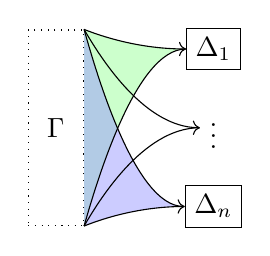
\begin{tikzpicture}[baseline]
    \path
    (-1,1) node (Gtop) {}
    (-1,0) node (G) {$\Gamma$}
    (-1,-1) node (Gbot) {}
    ;
    \node[draw,dotted,fit=(Gtop) (G) (Gbot)] (GG) {};

    \path
    (1,1) node[draw] (Dtop) {$\Delta_1$}
    (1,0) node (D) {$\vdots$}
    (1,-1) node[draw] (Dbot) {$\Delta_n$}
    ;

    \fill[green!20!white,opacity=1] (GG.north east)
    parabola[bend at end] (Dtop.west)
    parabola[bend at start] (GG.south east)
    -- cycle;
    \fill[blue!40!white,opacity=.5] (GG.north east)
    parabola[bend at end] (Dbot.west)
    parabola[bend at start] (GG.south east)
    -- cycle;

    \draw[->] (GG.north east) parabola[bend at end] (Dtop.west);
    \draw (GG.south east) parabola[bend at end] (Dtop.west);
    \draw[->] (GG.north east) parabola[bend at end] (D.west);
    \draw (GG.south east) parabola[bend at end] (D.west);
    \draw[->] (GG.north east) parabola[bend at end] (Dbot.west);
    \draw (GG.south east) parabola[bend at end] (Dbot.west);
  \end{tikzpicture}
\end{displaymath}

To account for usage, we must replace the simple repetition of $\Gamma$ by
repetition of just the types $\gamma$ and \emph{redistribution} of the usage
annotations $\grP$.
Fortunately, our three basic ways of sharing up usage vectors --- zero,
addition, and scaling --- apply directly to the three possible shapes of the
target context --- empty, concatenation, and a usage-annotated singleton.

\begin{definition}[Usage-annotated recursive environment]\label{def:lr-rec-env}
  A \emph{recursive $\V$-environment} between annotated contexts $\Gamma$ and
  $\Delta$ is defined by cases on the shape of $\Delta$ (where
  $\Gamma \env\V_R \Delta$ is the notation for the
  type of recursive environments for given $\V$, $\Gamma$, and $\Delta$):
  \begin{itemize}
    \item There is one environment $\alr{} : \grP\gamma \env\V_R {\cdot}$
      whenever $\grP \leq \gr0$.
    \item For $\rho_l : \grPl\gamma \env\V_R \Delta_l$ and
      $\rho_r : \grPr\gamma \env\V_R \Delta_r$, we have an environment
      $\alr{\rho_l, \rho_r} : \grP\gamma \env\V_R \Delta_l, \Delta_r$ whenever
      $\grP \leq \grPl + \grPr$.
    \item For any value $v : \V\,\grPprime\gamma\,A$, we have an environment
      $\alr{v} : \grP\gamma \env\V_R \gr rA$ whenever
      $\grP \leq \gr r\grPprime$.
  \end{itemize}
\end{definition}

\begin{example}
  Take $\Ann = \plr{\mathbb N, =, 0, +, 1, \times}$, with the equality order
  chosen to avoid any concerns around subsumption of annotations.
  Then, there is an intuitionistic recursive environment as follows, where
  $y\,z$ is the application of $y$ to $z$.
  \[
    \alr{\alr{z},\alr{y\,z}} :
    \plr{x : A, y : B \to C, z : B} \env\vdash_R \plr{B, C}.
  \]
  There is also a usage-aware recursive environment
  \[
    \alr{\alr{z},\alr{y\,z}} :
    \plr{\gr0x : A, \gr2y : B \multimap C, \gr3z : B} \env\vdash_R
    \plr{\gr1B, \gr2C}.
  \]
  The latter relies on the observations that
  $\begin{pmatrix} \gr0 & \gr2 & \gr3 \end{pmatrix} =
  \begin{pmatrix} \gr0 & \gr0 & \gr1 \end{pmatrix}
  + \begin{pmatrix} \gr0 & \gr2 & \gr2 \end{pmatrix}$ and, on the right, that
  $\begin{pmatrix} \gr0 & \gr2 & \gr2 \end{pmatrix} =
  \gr2\begin{pmatrix} \gr0 & \gr1 & \gr1 \end{pmatrix}$.
  Then, we have $\gr0x : A, \gr0y : B \multimap C, \gr1z : B \vdash z : B$ and
  $\gr0x : A, \gr1y : B \multimap C, \gr1z : B \vdash y\,z : C$.
\end{example}

From the example, we can see that the important usage vectors are the initial
one $\begin{pmatrix} \gr0 & \gr2 & \gr3 \end{pmatrix}$ and the usage vectors
at which terms are derived: $\begin{pmatrix} \gr0 & \gr0 & \gr1 \end{pmatrix}$
and $\begin{pmatrix} \gr0 & \gr1 & \gr1 \end{pmatrix}$.
I will call the latter the \emph{leaf vectors}.
The intermediate vector $\begin{pmatrix} \gr0 & \gr2 & \gr2 \end{pmatrix}$ can
be worked out from the leaf vector
$\begin{pmatrix} \gr0 & \gr1 & \gr1 \end{pmatrix}$ and the scaling factor
$\gr2$ found in the codomain context $\gr1B, \gr2C$.
Even when the ordering on annotations is given by a non-equivalence relation
$\leq$, there is a canonical least choice for all of the intermediate vectors,
together with a constraint that the entire linear combination of all the leaf
vectors is less than or equal to the initial usage vector.
In symbols, we may let $\gr\Psi$ be the collection of leaf vectors indexed by
items in $\Delta$, and state
the constraint as $\grP \leq \sum_{\plr{x : \gr rA} \in \Delta} \gr r\gr\Psi_x$.
Seeing $\gr\Psi$ instead as a $\size\Delta \times \size\Gamma$ matrix, this
constraint is $\grP \leq \grQ\gr\Psi$, using vector-matrix multiplication.
The resulting picture is below, showing $\grP$ being split up into $\gr\Psi$,
and then each $\V$-value being constructed in a separate $\gr\Psi_i\gamma$.

\begin{displaymath}
  \begin{tikzpicture}[baseline]
    \path
    (-1,1) node (Gtop) {}
    (-1,0) node (G) {$\grP\gamma$}
    (-1,-1) node (Gbot) {}
    ;
    \node[draw,dotted,fit=(Gtop) (G) (Gbot)] (GG) {};

    \path
    (1,1) node (Dtop) {}
    (1,0) node (D) {$\grQ\delta$}
    (1,-1) node (Dbot) {}
    ;
    \node[draw,dotted,fit=(Dtop) (D) (Dbot)] (DD) {};

    \draw[->,double] (GG) -- (DD);
  \end{tikzpicture}
  \coloneqq
  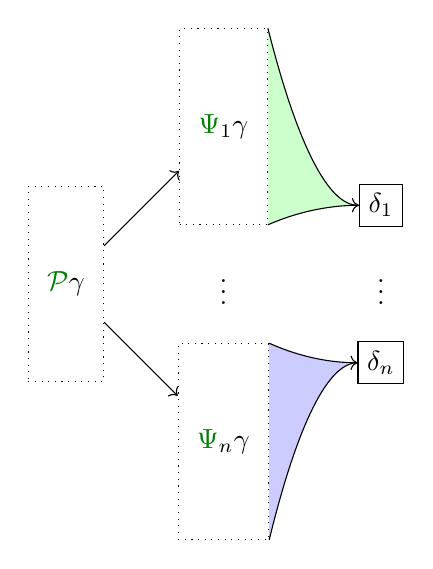
\begin{tikzpicture}[baseline]
    \path
    (-1,1) node (Gtop) {}
    (-1,0) node (G) {$\grP\gamma$}
    (-1,-1) node (Gbot) {}
    ;
    \node[draw,dotted,fit=(Gtop) (G) (Gbot)] (GG) {};

    \path
    (1,3) node (G1top) {}
    (1,2) node (G1) {$\gr\Psi_1\gamma$}
    (1,1) node (G1bot) {}
    ;
    \node[draw,dotted,fit=(G1top) (G1) (G1bot)] (GG1) {};
    \draw[->] (GG) -- (GG1);

    \path (1,0) node {$\vdots$};

    \path
    (1,-1) node (Gntop) {}
    (1,-2) node (Gn) {$\gr\Psi_n\gamma$}
    (1,-3) node (Gnbot) {}
    ;
    \node[draw,dotted,fit=(Gntop) (Gn) (Gnbot)] (GGn) {};
    \draw[->] (GG) -- (GGn);

    \path
    (3,1) node[draw] (Dtop) {$\delta_1$}
    (3,0) node (D) {$\vdots$}
    (3,-1) node[draw] (Dbot) {$\delta_n$}
    ;

    \fill[green!20!white] (GG1.north east)
    parabola[bend at end] (Dtop.west)
    parabola[bend at start] (GG1.south east)
    -- cycle;
    \draw[->] (GG1.north east) parabola[bend at end] (Dtop.west);
    \draw (GG1.south east) parabola[bend at end] (Dtop.west);

    \fill[blue!20!white] (GGn.north east)
    parabola[bend at end] (Dbot.west)
    parabola[bend at start] (GGn.south east)
    -- cycle;
    \draw[->] (GGn.north east) parabola[bend at end] (Dbot.west);
    \draw (GGn.south east) parabola[bend at end] (Dbot.west);
  \end{tikzpicture}
  \quad\textrm{where }\grP \leq \grQ\gr\Psi
\end{displaymath}

From this point, we can recover a functional-style definition of usage-aware
environments.
We choose our leaf vectors $\gr\Psi$ up-front, check the inequality, and then
produce a value at each leaf vector.
%From this definition, we can recover a functional-style definition by
%separating choices of usage vectors from the provision of $\V$-values.
%In particular, the only choices of usage vectors that are essential are the
%$\grPprime$s in the singleton case, with the choices in the concatenation case
%being determined as scalings and sums of these $\grPprime$s.
%I let $\gr\Psi$ collect up these $\size\Delta$-many choices of
%$\size\Gamma$-length usage vectors and note that the constraint on $\gr\Psi$
%generated by all the scaling and summing is
%$\grP = \sum_{\plr{x : \gr rA} \in \Delta} \gr r\gr\Psi_x$.

\begin{definition}[Usage-annotated environment (tentative)]
  A \emph{$\V$-environment} between annotated contexts $\Gamma$ and $\Delta$
  (written $\grP\gamma$ and $\grQ\delta$, respectively, when convenient)
  is a matrix $\gr\Psi : \Ann^{\size\Delta \times \size\Gamma}$ such that
  $\grP \leq \grQ\gr\Psi$ and for each
  $\plr{x : A} \in \delta$ we have a value of type $\V\,\gr\Psi_x\gamma\,A$.
\end{definition}

I find this definition somewhat fiddly because of its reliance on low-level
concepts like non-usage-checked variables and rows of a matrix.
We note that $\gr\Psi_x = \bra x\gr\Psi$, from which point, requiring not
just $\V\,\gr\Psi_x\gamma\,A$ but rather $\V\,\plr{\grQprime\gr\Psi}\gamma\,A$
for any $\grQprime \leq \bra x$ is a minor change (and equivalent if $\V$
respects subusaging, which is practically always the case).
``An $x$ such that $(x : A) \in \delta$ and $\grQprime \leq \bra x\gr\Psi$''
is exactly the definition of $\grQprime\delta \sqni A$.
I further regularise this clause by asking for a
$\grPprime \leq \grQprime\gr\Psi$ rather than $\grQprime\gr\Psi$ exactly,
leaving us needing, for each $\grPprime$ and $\grQprime$ related in the same
way ($\gr\Psi$) as $\grP$ and $\grQ$, a function from $\grQprime\delta \sqni A$
to $\V\,\grPprime\gamma\,A$.
Finally, I choose to switch from matrices and matrix multiplication to
linear maps and their actions, which are easier to work with.
All of these changes yield my primary definition of an environment for
usage-annotated calculi, which will be used for the rest of this chapter and in
\cref{sec:framework}.

\begin{definition}[Usage-annotated environment]\label{def:lr-env}
  A \emph{$\V$-environment} between annotated contexts $\Gamma$ and $\Delta$
  (written $\grP\gamma$ and $\grQ\delta$, respectively, when convenient)
  is a linear map $\gr\Psi : \Ann^{\size\Delta} \to \Ann^{\size\Gamma}$ (written
  postfix) such that $\grP \leq \grQ\gr\Psi$ and for each $A$, $\grPprime$, and
  $\grQprime$ such that $\grPprime \leq \grQprime\gr\Psi$, a function from
  $\grQprime\delta \sqni A$ to $\V\,\grPprime\gamma\,A$.
\end{definition}
\begin{notation}
  When there are multiple environments in question and $\rho$ is such an
  environment, I use the notation $\rho.\gr\Psi$ to refer to $\gr\Psi$.
  For example, $\grP \leq \grQ\plr{\rho.\gr\Psi}$.
  For the action on variables, I write $\rho(x)$, where
  $x : \grQprime\delta \sqni A$.
  The expression ``$\rho(x)$'' alone is ambiguous because of the slack in the
  usage context $\grPprime$ of the resulting value.
  Therefore, I will always make sure $\grPprime$ and $\grQprime$ clear when
  using this notation.
\end{notation}

The following simple lemma shows that usage-annotated environments are, in a
sense, as good as simple environments on usage-checked variables.
What usage-annotated environments give us beyond simple environments is the
ability to accommodate linear decompositions, in a way I will make precise in
the next section.

\begin{lemma}
  We can use an environment $\rho : \Gamma \env\V \Delta$ to map a
  usage-checked variable $x : \Delta \sqni A$ to a value of type
  $\V\,\Gamma\,A$.
\end{lemma}
\begin{proof}
  Let $\Gamma = \grP\gamma$ and $\Delta = \grQ\delta$.
  Set $\grPprime \coloneqq \grP$ and $\grQprime \coloneqq \grQ$, then
  $\grP \leq \grQ\gr\Psi$ by the constraint in $\rho$, so we can take
  the $\V$-value $\rho(x)$.
\end{proof}

\section{Properties of linear environments}\label{sec:lenv}
I settle on \cref{def:lr-env}, and prove various properties about it.

\begin{lemma}\label{thm:env-resize}
  Given an environment $\rho : \grP\gamma \env\V \grQ\delta$ and a $\grPprime$
  and a $\grQprime$ such that $\grPprime \leq \grQprime\plr{\rho.\gr\Psi}$,
  there is also an environment of type $\grPprime\gamma \env\V \grQprime\delta$
  with the same linear map and action on variables.
\end{lemma}
\begin{proof}
  The only part of the definition of an environment dependent on $\grP$ or
  $\grQ$ is the constraint $\grP \leq \grQ\gr\Psi$, which we are able to
  replace for $\grPprime$ and $\grQprime$.
\end{proof}

When constructing an environment, we can do so by cases on the shape of the
target context.
We can create an environment into the empty context when all usage annotations
on the source context are $\gr0$.
We can create an environment into a concatenated context when we can additively
split up the annotations of the source context and produce environments into
both halves from the split sources.
We can create an environment into a singleton context when there is a context
$\gr r$ times smaller than the source context in which we can produce a value
of the appropriate type.

\begin{lemma}\label{thm:construct-env}
  We can define all of the following equivalences for any values of the free
  variables, assuming that $\V$ respects subusaging (i.e.,
  $\grPprime \leq \grP \to
  \V\,\grP\gamma \rightarrowtriangle \V\,\grPprime\gamma$).
  \begin{itemize}
    \item $I^{\sep} \leftrightarrowtriangle \plr{{-} \env\V {\cdot}}$
    \item $\plr{{-} \env\V \Delta_l} \sep \plr{{-} \env\V \Delta_r}
      \leftrightarrowtriangle \plr{{-} \env\V \Delta_l, \Delta_r}$
    \item $\gr r \cdot \plr{\V\,(-)\,A}
      \leftrightarrowtriangle \plr{{-} \env\V \gr rA}$
  \end{itemize}
\end{lemma}
\begin{proof}
  There are 6 cases to check.
  Throughout, we write $\Gamma$ as $\grP\gamma$ and $\Delta$ as $\grQ\delta$
  when convenient.
  \begin{description}
    \item[$I^{\sep}(\rightarrowtriangle)$]
      Let $\gr\Psi$ be the unique linear map out of the zero space.
      By assumption and definition, $\grP \leq \gr0 = \grQ\gr\Psi$.
      There are no variables to act upon.
    \item[$I^{\sep}(\leftarrowtriangle)$]
      $\grQ\gr\Psi$ is an empty sum, so if $\grP \leq \grQ\gr\Psi$ then
      $\grP \leq \gr0$.
    \item[$\sep(\rightarrowtriangle)$]
      Let the given environments be $\rho_l : \grPl\gamma \env\V \grQl\delta$
      and $\rho_r : \grPr\gamma \env\V \grQr\delta$, with
      $\grP \leq \grPl + \grPr$.
      Define $\gr\Psi \coloneqq [\rho_l.\gr\Psi, \rho_r.\gr\Psi]$, using the
      coproduct structure of the concatenated vector space.
      We have $\grP \leq \grPl + \grPr \leq
      \grQl\plr{\rho_l.\gr\Psi} + \grQr\plr{\rho_r.\gr\Psi} =
      \begin{pmatrix} \grQl & \grQr \end{pmatrix}\gr\Psi$.
      To act on variables, we are given $\grPprime \leq
      \begin{pmatrix} \gr{\grQ'_l} & \gr{\grQ'_r} \end{pmatrix}\gr\Psi$ and
      $\gr{\grQ'_l}\delta_l, \gr{\grQ'_r}\delta_r \sqni A$.
      Without loss of generality, let us have $\gr{\grQ'_l}\delta_l \sqni A$
      and $\gr{\grQ'_r} \leq \gr0$.
      Thus, $\grPprime \leq
      \gr{\grQ'_l}\plr{\rho_l.\gr\Psi} + \gr{\grQ'_r}\plr{\rho_r.\gr\Psi} \leq
      \gr{\grQ'_l}\plr{\rho_l.\gr\Psi}$,
      and we can act on the variable using $\rho_l$.
    \item[$\sep(\leftarrowtriangle)$]
      Let the unnamed context be $\Gamma$, also written $\grP\gamma$.
      The linear map
      $\gr\Psi : \Ann^{\size{\Delta_l} + \size{\Delta_r}} \to \Ann^{\size\Gamma}$
      splits into
      $\gr\Psi_{\gr l} : \Ann^{\size{\Delta_l}} \to \Ann^{\size\Gamma}
      \coloneqq \alr{\id, 0}; \gr\Psi$ and
      $\gr\Psi_{\gr r} : \Ann^{\size{\Delta_r}} \to \Ann^{\size\Gamma}
      \coloneqq \alr{0, \id}; \gr\Psi$, using the product structure of
      the concatenated vector space.
      Let $\grPl \coloneqq \grQl\gr\Psi_{\gr l}$ and
      $\grPr \coloneqq \grQr\gr\Psi_{\gr r}$, by definition satisfying the
      required constraints.
      For the action on variables, let us consider the left environment (with
      the right environment following symmetrically).
      We are given $\gr{\grP'_l} \leq \gr{\grQ'_l}\gr\Psi_{\gr l}$ and
      $\gr{\grQ'_l}\delta_l \sqni A$.
      From these, we get
      $\gr{\grP'_l} \leq \gr{\grQ'_l}\gr\Psi_{\gr l} =
      \begin{pmatrix} \gr{\grQ'_l} & \gr0 \end{pmatrix}\gr\Psi$ and
      $\gr{\grQ'_l}\delta_l, \gr0\delta_r \sqni A$.
      We can therefore act using the original environment.
    \item[$\cdot(\rightarrowtriangle)$]
      Let $\grP$ and $\grPprime$ be such that $\grP \leq \gr r\grPprime$ and let
      $v : \V\,\grPprime\gamma\,A$.
      Let $\gr\Psi : \Ann \to \Ann^{\size\gamma}
      \coloneqq \gr r\gr' \mapsto \gr r\gr'\grPprime$.
      By definition and the previous assumption, we have
      $\grP \leq \gr r\gr\Psi$.
      When acting on a variable, we have $\grP\gr{''} \leq \gr r\gr'\gr\Psi$
      and $\gr r\gr'A \sqni A'$.
      The latter tells us that $A = A'$ and $\gr r\gr' \leq \gr1$.
      Thus, $\grP\gr{''} \leq \grPprime$.
      Therefore, by subusaging, we may produce a value of type
      $\V\,\grPprime\gamma\,A$, which we can take to be $v$.
    \item[$\cdot(\leftarrowtriangle)$]
      Let us have an environment of type $\grP\gamma \env\V \gr rA$.
      We want to use its action on variables to yield a value.
      To do this, we let $\grPprime \coloneqq \gr1\gr\Psi$, and use this
      equation, together with the fact that we have a variable of type
      $\gr1A \sqni A$, to get a value of type $\V\,\grPprime\gamma\,A$.
      Furthermore, we derive $\grP \leq \gr r\gr\Psi = \gr r\grPprime$, as
      required.
  \end{description}
\end{proof}

We could, as in \cref{def:lr-rec-env}, use these three clauses to define what an
environment is.
However, such a definition appears to require creative induction hypotheses in
the proving of simple lemmas, in contrast to the more direct proofs I achieve
below using \cref{def:lr-env}.
To take a concrete example, consider how we may construct an ``identity''
environment of type $\Gamma \env\V \Gamma$, as in \cref{thm:env-id} below.
If we try to directly proceed by induction on $\Gamma$, we get to the case where
we are aiming to construct an environment of type
$\grP\gamma, \grQ\delta \env\V \grP\gamma, \grQ\delta$ by constructing
environments of types $\grP\gamma, \gr0\delta \env\V \grP\gamma$ and
$\gr0\gamma, \grQ\delta \env\V \grQ\delta$.
These are not identity environments, and thus do not come from the hypotheses of
a simple induction.
In contrast, using \cref{def:lr-env}, in \cref{thm:env-id} we are able to use
the standard fact that there are identity linear maps, and on top of such a map
worry only about the value assigned to each variable.

One of the primary test cases for environments is simultaneous substitution,
which will look like the \TirName{sub} rule below.
Note that we have taken $\V \coloneqq {\vdash}$ --- i.e.\ that the values
yielded by the environment are terms, namely the terms to be substituted in for
the free variables of the derivation of $\Delta \vdash A$.

\begin{displaymath}
  \begin{prooftree}
    \hypo{\Gamma \env{\vdash} \Delta}
    \hypo{\Delta \vdash A}
    \infer2[sub]{\Gamma \vdash A}
  \end{prooftree}
\end{displaymath}

The admissibility of substitution will be by induction on the derivation of
$\Delta \vdash A$, so we will need to be able to adapt any environment we are
given to work with any possible context of new premises yielded by the rules of
\cref{fig:lr-bunched}.
In the simply typed case, the only change to the context we encountered was the
binding of new variables.
With usage annotations, we furthermore have linear decompositions of the
context, necessitating changes to the environment whenever usage annotations
change.

There are three kinds of linear decompositions we have to deal with: zero,
addition, and scaling; corresponding to bunched connectives $I^*$, $\sep$, and
$\gr r \cdot {}$, respectively.
In each of these three cases, we have a simple preservation lemma, transforming
an environment
of type $\Gamma \env\V \Delta$ and a decomposition of $\Delta$ into a
decomposition of $\Gamma$ and environments for all of the decomposed fragments
of $\Gamma$ and $\Delta$.

\begin{lemma}[environments preserve zero]\label{thm:lr-env-zero}
  Given an environment $\rho : \grP\gamma \env\V \grQ\delta$ such that
  $\grQ \leq \gr 0$, we also have that $\grP \leq \gr 0$.
\end{lemma}
\begin{proof}
  $\grP \leq \grQ\gr\Psi \leq \gr0\gr\Psi = \gr0$, by environment
  compatibility from $\rho$ and monotonicity and linearity of $\gr\Psi$.
\end{proof}

\begin{lemma}[environments preserve addition]\label{thm:lr-env-add}
  Given an environment $\rho : \grP\gamma \env\V \grQ\delta$ such that
  $\grQ \leq \grQl + \grQr$ for some $\grQl$ and $\grQr$, we also have $\grPl$
  and $\grPr$ such that $\grP \leq \grPl + \grPr$ and there are environments
  $\rho_l : \grPl\gamma \env\V \grQl\delta$ and
  $\rho_r : \grPr\gamma \env\V \grQr\delta$.
\end{lemma}
\begin{proof}
  Let $\grPl \coloneqq \grQl\gr\Psi$ and $\grPr \coloneqq \grQr\gr\Psi$.
  Then, $\grP \leq \grQ\gr\Psi \leq \plr{\grQl + \grQr}\gr\Psi =
  \grQl\gr\Psi + \grQr\gr\Psi = \grPl + \grPr$, satisfying the first condition.
  Because clearly $\grPl \leq \grQl\gr\Psi$ and $\grPr \leq \grQr\gr\Psi$,
  applying \cref{thm:env-resize} to $\rho$ gives us the required
  new environments $\rho_l$ and $\rho_r$.
\end{proof}

\begin{lemma}[environments preserve scaling]\label{thm:lr-env-scale}
  Given an environment $\rho : \grP\gamma \env\V \grQ\delta$ such that
  $\grQ \leq \gr r\grQprime$ for some $\grQprime$, we also have a $\grPprime$
  such that $\grP \leq \gr r\grPprime$ and there is an environment
  $\rho' : \grPprime\gamma \env\V \grQprime\delta$.
\end{lemma}
\begin{proof}
  Let $\grPprime \coloneqq \grQprime\gr\Psi$.
  Then, $\grP \leq \grQ\gr\Psi \leq \plr{\gr r\grQprime}\gr\Psi =
  \gr r\plr{\grQprime\gr\Psi} = \gr r\grPprime$, satisfying the first condition.
  Because clearly $\grPprime \leq \grQprime\gr\Psi$,
  applying \cref{thm:env-resize} to $\rho$ gives us the required
  new environment $\rho'$.
\end{proof}

The final change environments need to preserve is the binding of new free
variables.
In \cref{sec:syntactic-kits}, we had the operation \AgdaFunction{bindEnv} for
this purpose in the intuitionistic setting.
There, we relied on $\V$ supporting a map from $\ni$-variables and admitting
weakening.
In the usage-annotated setting, the former requirement is updated to having a
map from usage-checked $\sqni$-variables.
As for the latter requirement, it turns out that we only need $\V$ to admit
weakening by $\gr0$-annotated variables, which is much more reasonable than
general weakening.
\Cref{thm:lr-bind} adapts \AgdaFunction{bindEnv} for the usage-annotated
setting.

\begin{lemma}[\AgdaFunction{bindEnv}]\label{thm:lr-bind}
  Given functions
  ${\swarrow^k} : \forall \Gamma, \grR, \theta.~\grR \leq \gr0 \to
  \V\,\Gamma \rightarrowtriangle \V\,\plr{\Gamma, \grR\theta}$ and
  $\mathrm{vr} : {\sqni} \rightarrowtriangle \V$, we can turn an environment of
  type $\Gamma \env\V \Delta$ into an environment of type
  $\Gamma, \Theta \env\V \Delta, \Theta$ for any context $\Theta$.
\end{lemma}
\begin{proof}
  Let $\grP\gamma \coloneqq \Gamma$, $\grQ\delta \coloneqq \Delta$, and
  $\grR\theta \coloneqq \Theta$.
  Let the new linear map $\gr\Psi\gr' : \Ann^{\size\Delta + \size\Theta} \to
  \Ann^{\size\Gamma + \size\Theta}$ be $\gr\Psi \oplus \gr I$.
  That is, in block matrix notation,
  $\begin{pmatrix} \gr\Psi & \gr0 \\ \gr0 & \gr I \end{pmatrix}$.
  Checking that this linear map fits, we have
  $\begin{pmatrix}\grP & \grR\end{pmatrix}
  \leq \begin{pmatrix}\grQ\gr\Psi & \grR\gr I\end{pmatrix}
  = \begin{pmatrix}\grQ & \grR\end{pmatrix}\plr{\gr\Psi \oplus \gr I}$.
  For the action on variables, we are given vectors $\grPprime$,
  $\grR\gr'_\grP$, $\grQprime$, and $\grR\gr'_\grQ$ such that
  $\begin{pmatrix} \grPprime & \grR\gr'_\grP \end{pmatrix} \leq
  \begin{pmatrix} \grQprime & \grR\gr'_\grQ \end{pmatrix}
  \plr{\gr\Psi \oplus \gr I}$ and we have a variable of type
  $\grQprime\delta, \grR\gr'_\grQ\theta \sqni A$ for some type $A$.
  The constraint on the new vectors reduces to $\grPprime \leq \grQprime\gr\Psi$
  and $\grR\gr'_\grP \leq \grR\gr'_\grQ$.
  From the variable we either have a variable $x$ in $\delta$ with
  $\grQprime \leq \langle x \rvert$ and $\grR\gr'_\grQ \leq \gr0$, or a
  variable $y$ in $\theta$ with $\grQprime \leq \gr0$ and
  $\grR\gr'_\grQ \leq \langle y \rvert$.
  In the former case, the action of the original environment on $x$ gives us a
  $\V$-value in $\grPprime\gamma$, and the $\gr0$-weakening principle
  $\swarrow^k$, noting that $\grR\gr'_\grP \leq \grR\gr'_\grQ \leq \gr0$, gives
  us a $\V$-value in $\grPprime\gamma, \grR\gr'_\grP\theta$.
  In the latter case, we have that
  $\begin{pmatrix} \grPprime & \grR\gr'_\grP \end{pmatrix}
  \leq \begin{pmatrix} \grQprime\gr\Psi & \grR\gr'_\grQ \end{pmatrix}
  \leq \begin{pmatrix} \gr0\gr\Psi & \langle y \rvert \end{pmatrix}
  = \begin{pmatrix} \gr0 & \langle y \rvert \end{pmatrix}
  = \left\langle {\searrow}y \right\rvert$, so $y$ also serves as a
  usage-checked variable in $\grPprime\gamma, \grR\gr'_\grP\theta$.
  From this usage-checked variable, we get a $\V$-value in the same context
  using $\mathrm{vr}$.
\end{proof}

I put together the preceding pieces to give a syntactic traversal operation over
$\name$ in the following section.
For the rest of this section, I observe some more constructions purely on
environments --- in particular, composition of environments given certain
assumptions about the families of values.

Following \citet{ACU15}, we expect (intuitionistic) ST$\lambda$C syntax to form
a relative monad over $\ni$ seen as a functor from the category of contexts
under renaming to the functor category $\blr{\mathrm{Ty}, \Set}$, where
$\mathrm{Ty}$ is the discrete category of ST$\lambda$C types.
Notice that, given $F,G : \blr{\mathrm{Ty}, \Set}$, a morphism from $F$ to $G$
is a function of type $F \rightarrowtriangle G$ (with naturality being trivial).
Therefore, we expect a relative monad, given as a Kleisli triple, to have a unit
$\eta_\Gamma : \Gamma \ni \plr{-} \rightarrowtriangle \Gamma \vdash \plr{-}$
given by the variable rule, and a Kleisli extension operator
${^*}_{\Gamma,\Delta} :
\plr{\Gamma \ni \plr{-} \rightarrowtriangle \Delta \vdash \plr{-}} \to
\plr{\Gamma \vdash \plr{-} \rightarrowtriangle \Delta \vdash \plr{-}}$
given by substitution.
Composition of substitutions falls out of this framework as Kleisli composition.
However, in the usage-aware case, substitution needs not just a mapping of
variables $f : \Gamma \sqni \plr{-} \rightarrowtriangle \Delta \vdash \plr{-}$,
but rather an environment $\rho : \Delta \env\vdash \Gamma$, as we have already
discussed.
It therefore makes sense for our replacement for the Kleisli extension operator
to similarly take an environment rather than a simple variable mapping.

\Cref{thm:env-comp} below amounts to deriving a modified notion of Kleisli
composition from a modified Kleisli extension.
Additionally, \cref{thm:env-id} is required to turn a monadic unit into an
identity environment.
Both lemmas are stated in terms of general $\U$/$\V$/$\W$-environments, with
some specific examples (e.g.\ for renaming and substitution) below them.

\begin{lemma}[Identity environment]\label{thm:env-id}
  Given a function
  \[
    \mathrm{vr}_{\Gamma'} :
    \Gamma' \sqni \plr{-} \rightarrowtriangle \V\,\Gamma'
  \]
  for any
  $\Gamma$ we have an environment $\mathrm{id} : \Gamma \env\V \Gamma$.
\end{lemma}
\begin{proof}
  Let $\Gamma = \grP\gamma$.
  Let $\gr\Psi$ be the identity map, which clearly satisfies
  $\grP \leq \grP\gr\Psi$.
  When acting on a variable, the inequality $\grPprime \leq \grQprime\gr\Psi$
  means that $\grPprime \leq \grQprime$.
  We are given a variable of type $\grQprime\gamma \sqni A$, which we can
  coerce to a variable of type $\grPprime\gamma \sqni A$, upon which we apply
  $\mathrm{vr}$ to get the required value of type $\V\,\grPprime\gamma\,A$.
\end{proof}

\begin{lemma}[Composition of environments]\label{thm:env-comp}
  Given a function
  \[
    \mathrm{lift}_{\Gamma', \Delta'} :
    \Gamma' \env\U \Delta' \to \V\,\Delta' \rightarrowtriangle \W\,\Gamma'
  \]
  we can compose environments $\rho : \Gamma \env\U \Delta$ and
  $\sigma : \Delta \env\V \Theta$ into an environment
  $\rho \gg \sigma : \Gamma \env\W \Theta$.
\end{lemma}
\begin{proof}
  Let $\Gamma = \grP\gamma$, $\Delta = \grQ\delta$, and $\Theta = \grR\theta$.
  Take $\gr\Psi$ to be the composition $\plr{\sigma.\gr\Psi}\plr{\rho.\gr\Psi}$,
  noting that
  $\grP \leq \grQ\plr{\rho.\gr\Psi} \leq
  (\grR\plr{\sigma.\gr\Psi})\plr{\rho.\gr\Psi} = \grR\gr\Psi$
  thanks to the inequalities yielded by $\sigma$ and $\rho$.
  When acting on a variable, we are given $\grPprime \leq \grRprime\gr\Psi$ and
  a variable $v : \grRprime\theta \sqni A$, and want a value of type
  $\W\,\grPprime\gamma\,A$.
  Let $\grQprime \coloneqq \grRprime\plr{\sigma.\gr\Psi}$, with inequality
  $\grQprime \leq \grRprime\plr{\sigma.\gr\Psi}$ giving us a value
  $\sigma(v) : \V\,\grQprime\delta\,A$.
  We wish to apply $\mathrm{lift}$ to $\sigma(v)$ with
  $\Gamma' \coloneqq \grPprime\gamma$ and $\Delta' \coloneqq \grQprime\delta$ to
  complete the construction of the $\W$-value.
  To do this, we need an environment of type
  $\grPprime\gamma \env\U \grQprime\delta$, which we can get from $\rho$ using
  \cref{thm:env-resize}, noting that
  $\grPprime \leq \grRprime\plr{\sigma.\gr\Psi}\plr{\rho.\gr\Psi} =
  \grQprime\plr{\rho.\gr\Psi}$.
\end{proof}

We can derive the following corollaries as instances of environment composition.

\begin{corollary}[Composition of renamings]\label{thm:ren-comp}
  Given renamings $\rho : \Gamma \env\sqni \Delta$ and
  $\sigma : \Delta \env\sqni \Theta$, we can form their composite
  $\rho; \sigma : \Gamma \env\sqni \Theta$.
\end{corollary}
\begin{proof}
  Take $\U = \V = \W = {\sqni}$ in \cref{thm:env-comp}.
  Then let $\mathrm{lift}\,\rho\,x \coloneqq \rho(x)$.
\end{proof}

\begin{corollary}[Post-composition with a renaming]\label{thm:ren-env-comp}
  Given an environment $\rho : \Gamma \env\U \Delta$ and a renaming
  $\sigma : \Delta \env\sqni \Theta$, we can form their composite
  $\rho; \sigma : \Gamma \env\U \Theta$.
\end{corollary}
\begin{proof}
  As in \cref{thm:ren-comp}.
\end{proof}

\begin{corollary}[Pointwise renaming of an environment]\label{thm:env-ren}
  If $\sdtstile{}\V$ respects renaming, then so does $\env\V$ (on the left).
\end{corollary}
\begin{proof}
  Suppose we have $\rho : \Gamma \env\sqni \Delta$ and
  $\sigma : \Delta \env\V \Theta$.
  We want to compose these via \cref{thm:env-comp} with $U = {\sqni}$ and
  $\V = \W$.
  The function $\mathrm{lift}$ is given exactly by the fact that $\V$ respects
  renaming.
\end{proof}

\begin{corollary}[Composition of substitutions]\label{thm:sub-comp}
  Given substitutions $\rho : \Gamma \env\vdash \Delta$ and
  $\sigma : \Delta \env\vdash \Theta$, we can form their composite
  $\rho; \sigma : \Gamma \env\vdash \Theta$.
\end{corollary}
\begin{proof}
  Take $\U = \V = \W = {\vdash}$ in \cref{thm:env-comp}.
  Then, $\mathrm{lift}$ is given by the action of a substitution on a term
  (see \AgdaFunction{sub} in the following section).
\end{proof}

\begin{corollary}[Composing semantics with substitution]
  If we have a semantics (in the sense of \cref{sec:gen-sem} and
  \cref{sec:traversal}) from $\U$ to $\W$, then from an environment
  $\rho : \Gamma \env\U \Delta$ and a substitution
  $\sigma : \Delta \env\vdash \Theta$, we can form the composite
  $\rho; \sigma : \Gamma \env\W \Theta$.
\end{corollary}

% Concatenation is difficult; save to after I've talked about renamings.

% Finally for this section, we give the conditions under which the
% context-forming operations (empty, concatenation, and singleton) have a
% functorial action with respect to $\V$-environments.
%
% \begin{lemma}
%   For any $\V$, there is an environment ${\cdot} \env\V {\cdot}$.
% \end{lemma}
% \begin{proof}
%   By \cref{thm:construct-env}, it suffices to show $I\,{\cdot}$, which is
%   trivially true.
% \end{proof}

\section{Substitution is admissible in \name{}}\label{sec:lrsub}
\def\LRKits{../agda/processed-latex/LRKits.tex}

I now show that, using the notion of \emph{environment} derived in
\cref{sec:lrkits}, we can replicate the Agda proofs from
\cref{sec:syntactic-kits} in the usage-aware setting of $\name$.
From \cref{sec:lenv}, we know that environments are preserved under all
syntax-forming operations: zero, addition, scaling, and binding.
What is left is to show how these properties are deployed, and also how to
go on and prove the admissibility of simultaneous renaming, simultaneous
substitution, and then single substitution.

There are a few notational changes necessary in the Agda code, compared to the
typeset mathematics above.
Usage vectors, elsewhere called $\grP$, $\grQ$, and $\grR$ are rendered as
\AgdaBound{P}, \AgdaBound{Q}, and \AgdaBound{R}, respectively.
Usage contexts and typing contexts are tied together with the
\AgdaInductiveConstructor{ctx} constructor, rather than simple juxtaposition.
Environments, elsewhere notated $\Gamma \env\V \Delta$, are rendered as
\AgdaRecord{[}\AgdaSpace{}\AgdaBound{$\V$}\AgdaSpace{}\AgdaRecord{]}%
\AgdaSpace{}\AgdaBound{$\Gamma$}\AgdaSpace{}\AgdaRecord{$\Rightarrow^e$}%
\AgdaSpace{}\AgdaBound{$\Delta$}.

I start with the definition \AgdaFunction{Weakening}, which says what it means
for a family of values \AgdaBound{$\V$} to respect one step of weakening on the
right by $\gr0$-use variables.
I state weakening in a slightly different way to what appears in the statement
of \cref{thm:lr-bind}, so as to help
unification against a known result type (avoiding the problem described by
\citet{McBride12} as \emph{green slime}).
The type \AgdaFunction{Weakening}\AgdaSpace{}\AgdaBound{$\V$} can be read as
saying that, for any context $\grP\gamma$ of shape $s + t$, if the right of
$\grP$ is below $\gr0$, then a value in the left part of $\grP\gamma$ weakens
to a value in the whole of $\grP\gamma$.

\ExecuteMetaData[\LRKits]{Weakening}

Given this new definition of \AgdaFunction{Weakening}, the record
\AgdaRecord{Kit} remains largely unchanged relative to what we saw in
\cref{sec:syntactic-kits}.
We still want $\V$-values to respect weakening (as used in \cref{thm:lr-bind}),
and to support maps \AgdaField{vr} from variables (also used in
\cref{thm:lr-bind}) and \AgdaField{tm} into terms (used when traversal reaches a
variable, we get a value from the environment, and want to produce a term from
that value).
As well as \AgdaFunction{Weakening}, note that \AgdaRecord{\_$\sqni$\_} and, of
course, \AgdaDatatype{\_$\vdash$\_} have different definitions to the
corresponding intuitionistic notions, but they still represent morally the same
parts of the language and its metatheory.

\ExecuteMetaData[\LRKits]{Kit}

To demonstrate the important points succinctly, I cut \name{} down to just the
$\oc\gr r$-fragment.
The introduction rule and pattern-matching eliminator feature scaling, addition,
and variable binding, missing out only on sharing (which is trivial) and zero
(which is simpler than, and analogous to, addition).
The resulting type of well typed terms is below.

\ExecuteMetaData[\LRKits]{Tm}

Given a \AgdaRecord{Kit}\AgdaSpace{}\AgdaBound{$\V$},
\cref{thm:lr-bind} gives a function with the following type.

\ExecuteMetaData[\LRKits]{bindEnv}

Given \AgdaFunction{bindEnv} (\cref{thm:lr-bind}), \AgdaFunction{env-+}
(\cref{thm:lr-env-add}), and \AgdaFunction{env-*} (\cref{thm:lr-env-scale}),
we can reproduce the syntactic traversal \AgdaFunction{trav}.
Similarly to the unchanged high-level definition of \AgdaRecord{Kit}, we are
aiming for an unchanged traversal principle expressed by the rule below.
When $\V$ has a \AgdaRecord{Kit} structure, and we have a $\V$-environment from
$\Gamma$ to $\Delta$, we can transform a term in $\Delta$ to a term in $\Gamma$
of the same type.

\[
  \begin{prooftree}
    \hypo{\text{\AgdaRecord{Kit}\AgdaSpace{}}\V}
    \hypo{\Gamma \env\V \Delta}
    \hypo{\Delta \vdash A}
    \infer3[Trav]{\Gamma \vdash A}
  \end{prooftree}
\]

With all the lemmas of \cref{sec:lenv} in place, writing \AgdaFunction{trav}
becomes routine.
When processing a rule, we work our way up through the
premise connectives, applying \AgdaFunction{env-*} wherever we see a
\AgdaFunction{$\cdot^c$}, \AgdaFunction{env-+} wherever we see a
\AgdaFunction{$*^c$}, and \AgdaFunction{bindEnv} wherever we see a
\AgdaFunction{Bind}.
We then use whatever environments (with names beginning with
\AgdaBound{$\rho$}) and whatever usage vector splitting facts (with names
beginning with \AgdaBound{sp}) come out of this process to recursively
traverse the subterms and recombine the results.

\ExecuteMetaData[\LRKits]{trav}

Instantiating the generic syntactic traversal \AgdaFunction{trav} to renaming
looks just like it did in the intuitionistic case.
I have consistently replaced intuitionistic variables by linear variables, so
\AgdaFunction{id} and \AgdaInductiveConstructor{var} still work to embed
variables into variables and terms, respectively.
Weakening for variables \AgdaFunction{$\swarrow^v$} (not pictured) has been
updated to note that, for $\grP \leq \bra x$ and $\grR \leq \gr0$, we also have
$\begin{pmatrix} \grP & \grR \end{pmatrix} \leq \bra{{\swarrow}x}$.

\ExecuteMetaData[\LRKits]{var-kit}

In the intuitionistic case, environments were just functions, so we passed the
variable weakening function \AgdaFunction{$\swarrow^v$} to the function
\AgdaFunction{ren} to yield a term weakening function.
However, a usage-aware environment is a function packed together with usage
distribution data.
As such, we must make an environment version of \AgdaFunction{$\swarrow^v$}.
I start with a general lemma \AgdaFunction{$\swarrow$\^{}Env}, stating that if
$\V$ supports weakening, then so do $\V$-environments (in their domain
context).
This lemma then specialises to variables, with the identity renaming
\AgdaFunction{id\^{}Env} on the left part of the context and the proof
\AgdaBound{R0} that the right part of the context is below $\gr0$ combining
to give the desired weakening environment.

\ExecuteMetaData[\LRKits]{dlv-env}

This is what we need to instantiate \AgdaFunction{trav} for substitution.
As a reminder, I also give the type of \AgdaFunction{sub} in rule form.

\ExecuteMetaData[\LRKits]{sub}
\[
  \ebrule{%
    \hypo{\Gamma \env\vdash \Delta}
    \hypo{\Delta \vdash B}
    \infer2[sub]{\Gamma \vdash B}
  }
\]

Finally, the simultaneous substitution \AgdaFunction{sub} specialises to
single substitution.

\begin{corollary}[Single substitution]\label{thm:single-sub}
  The following equivalent rules are admissible.
  \begin{mathpar}
    \ebrule{%
      \hypo{\grR \leq \gr r\grP + \grQ}
      \hypo{\grP\gamma \vdash A}
      \hypo{\grQ\gamma, \gr rA \vdash B}
      \infer3{\grR\gamma \vdash B}
    }
    \and
    \ebrule[comb]{%
      \hypo{\gr r \cdot \plr{{} \vdash A}}
      \hypo{\sep}
      \hypo{\gr rA \vdash B}
      \infer3{{} \vdash B}
    }
  \end{mathpar}
\end{corollary}
\begin{proof}
  It is enough to construct a substitution of type
  $\grR\gamma \env\vdash \grQ\gamma, \gr rA$.
  To do this, we use \cref{thm:construct-env} cases $\sep(\rightarrowtriangle)$
  and $\cdot(\rightarrowtriangle)$ on inequalities
  $\grR \leq \grQ + \gr r\grP$ and $\gr r\grP \leq \gr r\grP$ respectively to
  leave us needing a substitution of type $\grQ\gamma \env\vdash \grQ\gamma$ and
  a term of type $\grP\gamma \vdash A$.
  For the substitution, we give the identity substitution (\cref{thm:env-id}),
  and we have the term as a hypothesis.
\end{proof}

\section{Adding recursion to \name{}}\label{sec:rec}
Based on an intuitive understanding of ``usage'', recursion introduces a new
phenomenon relative to the forms of programs we have seen so far:
terms can be used an unbounded number of times.
For example, notice the following reduction in Agda.

\missingfigure{\texttt{foldr \_+\_ 0 (1 :: 2 :: 3 :: []) = 1 + (2 + (3 + 0))}}

The function \AgdaFunction{\_+\_} has been copied into 3 different places in
the running of the program.
This copying is despite no type telling us that \AgdaFunction{\_+\_} would be
used 3 times (both \verb|[1,2,3]| and \verb|[2,3]| have type
\AgdaDatatype{List}\AgdaSpace{}\AgdaDatatype{$\mathbb N$}, despite the
corresponding folds using \AgdaFunction{\_+\_} a different number of times).
As such, when checking an application of \AgdaFunction{foldr}, we need check
that we can use its functional argument (\AgdaFunction{\_+\_} in this case) an
arbitrary number of times.
If we were to fix $\Ann$ as the $\{\gr0, \gr1, \gr\omega\}$ posemiring, then
wrapping the type of the functional argument in $\oc\gr\omega$ would suffice.
However, we want to remain generic in the choice of semiring.

I propose the following additions to \name{} to support a broad class of
inductive types.
I define strictly positive functors syntactically, with the only notable
restriction being not being allowed to use the type variable $X$ in the domain
of a function type.
I then add least fixed points of such strictly positive functors to the syntax
of types.

\begin{align*}
  U &\Coloneqq A \multimap (-) \mid \oc\gr r(-) \\
  {\odot} &\Coloneqq {\otimes} \mid {\oplus} \mid {\with} \\
  F[X], G[X] &\Coloneqq X \mid A \mid U(F[X]) \mid F[X] \odot G[X] \\
  A &\Coloneqq \cdots \mid \mu X.~F[X]
\end{align*}

\begin{example}
  We may define $\mathrm{List}_A \coloneqq \mu X.~I \oplus \plr{A \otimes X}$.
\end{example}

In the typing rules, introduction of an inductive type is standard.
For the elimination rule, we follow a similar pattern to other pattern-matching
rules --- $\oplus$-E, $\otimes$-E, and $\oc$-E --- by splitting the context
and typing the eliminand in one half ($\grP$).
We type the continuation in the other half, but because the continuation may
be used multiple times, and in a modal context, we require that $\grQ$ is
preserved by all linear operations.

\begin{displaymath}
  \begin{prooftree}
    \hypo{\grR\gamma \vdash F[\mu X.~F[X]]}
    \infer1[$\mu$-I]{\grR\gamma \vdash \mu X.~F[X]}
  \end{prooftree}
\end{displaymath}
\begin{displaymath}
  \begin{prooftree}
    \hypo{\grR \leq \grP + \grQ}
    \hypo{\grP\gamma \vdash \mu X.~F[X]}
    \hypo{%
      \begin{matrix*}[l]
        \grQ \leq \gr0 \\
        \grQ \leq \grQ + \grQ \\
        \forall \gr r.~\grQ \leq \gr r\grQ
      \end{matrix*}%
    }
    \hypo{\grQ\gamma, \gr1F[C] \vdash C}
    \infer4[$\mu$-E]{\grR\gamma \vdash C}
  \end{prooftree}
\end{displaymath}

\begin{example}\label{thm:list-rules}
  For lists, we can derive the following introduction and elimination rules
  (with usage constraints omitted for brevity when obvious).

  \begin{align*}
    \begin{prooftree}
      \hypo{\grR \leq \gr0}
      \infer1[$I$-I]{I}
      \infer1[$\oplus$-I$_0$]%
      {\grR\gamma \vdash I \oplus \plr{A \otimes \mathrm{List}_A}}
      \infer1[$\mu$-I]{\grR\gamma \vdash \mathrm{List}_A}
    \end{prooftree}
    &&
    \begin{prooftree}
      \hypo{\grR \leq \grP + \grQ}
      \hypo{\grP\gamma \vdash A}
      \hypo{\grQ\gamma \vdash \mathrm{List}_A}
      \infer3[$\otimes$-I]{\grR\gamma \vdash A \otimes \mathrm{List}_A}
      \infer1[$\oplus$-I$_1$]%
      {\grR\gamma \vdash I \oplus \plr{A \otimes \mathrm{List}_A}}
      \infer1[$\mu$-I]{\grR\gamma \vdash \mathrm{List}_A}
    \end{prooftree}
  \end{align*}
  \begin{displaymath}
    \begin{prooftree}
      \hypo{\grP\gamma \vdash \mathrm{List}_A}
      \infer0[Var]{\gr0\gamma, \gr1\plr{I \oplus \plr{A \otimes C}}
        \vdash I \oplus \plr{A \otimes C}}
      \hypo{\nabla^n}
      \hypo{\nabla^c}
      \infer3[$\oplus$-E]{\grQ\gamma, \gr1\plr{I \oplus \plr{A \otimes C}}
        \vdash C}
      \infer2[$\mu$-E]{\grR\gamma \vdash C}
    \end{prooftree}
  \end{displaymath}
  \begin{align*}
    \textrm{where }\nabla^n &\coloneqq
    \begin{prooftree}
      \infer0[Var]{\gr0\gamma, \gr1I \vdash I}
      \hypo{\grQ\gamma \vdash C}
      \infer1[Wk]{\grQ\gamma, \gr0I \vdash C}
      \infer2[$I$-E]{\grQ\gamma, \gr1I \vdash C}
      \infer1[Wk]{\grQ\gamma, \gr0\plr{I \oplus \plr{A \otimes C}}, \gr1I
        \vdash C}
    \end{prooftree}
    \\\\
    \textrm{and }\nabla^c &\coloneqq
    \begin{prooftree}
      \infer0[Var]{\gr0\gamma, \gr1\plr{A \otimes C} \vdash A \otimes C}
      \hypo{\grQ\gamma, \gr1A, \gr1C \vdash C}
      \infer1[Wk]{\grQ\gamma, \gr0\plr{A \otimes C}, \gr1A, \gr1C \vdash C}
      \infer2[$\otimes$-E]{\grQ\gamma, \gr1\plr{A \otimes C} \vdash C}
      \infer1[Wk]%
      {\grQ\gamma, \gr0\plr{I \oplus \plr{A \otimes C}}, \gr1\plr{A \otimes C}
        \vdash C}
    \end{prooftree}
  \end{align*}
\end{example}

Following \cref{sec:lnd}, I want to turn the ad hoc constraints on $\grP$,
$\grQ$, and $\grR$ into the result of some premise combinators.
To do this, I introduce a new combinator $\Box^{0{+}{\times}}$ defined below,
along with the resulting implicit-context typing rules.

\begin{align*}
  \plr{\Box^{0{+}{\times}}\,T}\grR \coloneqq
  \plr{\grR \leq \gr0} \times \plr{\grR \leq \grR + \grR} \times
  \plr{\forall \gr r.~\grR \leq \gr r\grR} \times T\,\grR
\end{align*}

\begin{align*}
  \begin{prooftree}[comb]
    \hypo{\vdash F[\mu X.~F[X]]}
    \infer1[$\mu$-I]{\vdash \mu X.~F[X]}
  \end{prooftree}
  &&
  \begin{prooftree}[comb]
    \hypo{\vdash \mu X.~F[X]}
    \hypo{\sep}
    \hypo{\Box^{0{+}{\times}}\plr{\gr1F[C] \vdash C}}
    \infer3[$\mu$-E]{\vdash C}
  \end{prooftree}
\end{align*}

\begin{example}
  We can state the rules for lists derived in \cref{thm:list-rules} as follows.
  \begin{align*}
    \begin{prooftree}[comb]
      \hypo{I^*}
      \infer1{\vdash \mathrm{List}_A}
    \end{prooftree}
    &&
    \begin{prooftree}[comb]
      \hypo{\vdash A}
      \hypo{\sep}
      \hypo{\vdash \mathrm{List}_A}
      \infer3{\vdash \mathrm{List}_A}
    \end{prooftree}
    &&
    \begin{prooftree}[comb]
      \hypo{\vdash \mathrm{List}_A}
      \hypo{\sep}
      \hypo{\Box^{0{+}{\times}}
        \plr{\vdash C\hskip0.75em\dottimes\hskip0.75em\gr1A, \gr1C \vdash C}}
      \infer3{\vdash C}
    \end{prooftree}
  \end{align*}
\end{example}

\section{Addendum: (lack of) partiality}\label{sec:part}
As we have seen, the way additive and multiplicative rules are
realised algebraically is related to models of separation logic.
Models of separation logic typically use \emph{partial} commutative monoids to
model a heap, so it is tempting to generalise the commutative monoid of
addition in our semirings to a \emph{partial} commutative monoid.
However, we find that the most natural notion of \emph{partial semiring} is
degenerate, in the sense that all partial semirings are actually (total)
semirings.

Recall that a commutative monoid (or commutative monoid object) can be
defined in any symmetric monoidal category.
A partial commutative monoid is exactly a commutative monoid object in the
category of sets and partial functions with the usual monoidal product given
by pairing of objects and morphisms (like the Cartesian product in $\Set$).
However, semirings need a Cartesian category in order to state the interaction
equations between addition and multiplication.
While the category of sets and partial functions is not Cartesian, the
standard way to manufacture a Cartesian category out of a symmetric monoidal
category $\mathcal C$ is to take the category of cocommutative comonoids
$\mathrm{CComon}(\mathcal C)$.
Intuitively, the cocommutative comonoid structure equips the underlying
object $M$ with a \emph{delete} map $\eta : M \to I$ and a \emph{duplicate}
map $\delta : M \to M \otimes M$ which are coherent with respect to each other.
All morphisms in $\mathrm{CComon}(\mathcal C)$ must respect $\eta$ and
$\delta$; in particular, both addition and multiplication must separately
form bimonoids in $\mathcal C$ together with the cocommutative comonoid.

The distributivity laws of semirings are stated below.
I include these to show that the cocommutative comonoids of a monoidal category
give enough structure to state these laws.
The other laws --- that all morphisms respect $\eta$ and $\delta$, that addition
forms a commutative monoid, and that multiplication forms a monoid --- are
standard in symmetric monoidal category theory.

\[
  \begin{tikzpicture}[baseline]
    \path
    (-1,1) node(0) {0}
    (1,2) node(x) {}
    (0,0) node(*) {*}
    (0,-1) node(res) {}
    ;

    \draw (0) -- (*);
    \draw (x) to[out=270,in=45] (*);
    \draw (*) -- (res);
  \end{tikzpicture}
  =\quad
  \begin{tikzpicture}[baseline]
    \path
    (0,0) node(0) {0}
    (0,2) node(x) {}
    (0,-1) node(res) {}
    (0,1) node(del) {$\eta$}
    ;

    \draw (0) -- (res);
    \draw (x) -- (del);
  \end{tikzpicture}
  \quad=
  \begin{tikzpicture}[baseline]
    \path
    (1,1) node(0) {0}
    (-1,2) node(x) {}
    (0,0) node(*) {*}
    (0,-1) node(res) {}
    ;

    \draw (0) -- (*);
    \draw (x) to[out=270,in=135] (*);
    \draw (*) -- (res);
  \end{tikzpicture}
\]
\begin{displaymath}
  \begin{matrix}
    \begin{tikzpicture}[baseline]
      \path
      (-1,2) node(x) {}
      (0,2) node(y) {}
      (-0.5,1) node(+) {+}
      (1,2) node(z) {}
      (0,0) node(*) {*}
      (0,-1) node(res) {}
      ;

      \draw (x) to[out=270,in=135] (+);
      \draw (y) to[out=270,in=45] (+);
      \draw (+) to[out=270,in=135] (*);
      \draw (z) to[out=270,in=45] (*);
      \draw (*) -- (res);
    \end{tikzpicture}
    =
    \begin{tikzpicture}[baseline]
      \path
      (-2,3) node(x) {}
      (-1,3) node(y) {}
      (0,3) node(z) {}
      (0,2) node(dup) {$\delta$}
      (-1,1) node(x*) {*}
      (0,1) node(y*) {*}
      (-0.5,0) node(+) {+}
      (-0.5,-1) node(res) {}
      ;

      \draw (z) -- (dup);
      \draw (x) to[out=270,in=135] (x*);
      \draw (y) to[out=270,in=135] (y*);
      \draw (dup) to[out=-150,in=45] (x*);
      \draw (dup) -- (y*);
      \draw (x*) to[out=270,in=135] (+);
      \draw (y*) to[out=270,in=45] (+);
      \draw (+) -- (res);
    \end{tikzpicture}
    &\phantom{mmmm}&
    \begin{tikzpicture}[baseline]
      \path
      (1,2) node(x) {}
      (0,2) node(y) {}
      (0.5,1) node(+) {+}
      (-1,2) node(z) {}
      (0,0) node(*) {*}
      (0,-1) node(res) {}
      ;

      \draw (x) to[out=270,in=45] (+);
      \draw (y) to[out=270,in=135] (+);
      \draw (+) to[out=270,in=45] (*);
      \draw (z) to[out=270,in=135] (*);
      \draw (*) -- (res);
    \end{tikzpicture}
    =
    \begin{tikzpicture}[baseline]
      \path
      (2,3) node(x) {}
      (1,3) node(y) {}
      (0,3) node(z) {}
      (0,2) node(dup) {$\delta$}
      (1,1) node(x*) {*}
      (0,1) node(y*) {*}
      (0.5,0) node(+) {+}
      (0.5,-1) node(res) {}
      ;

      \draw (z) -- (dup);
      \draw (x) to[out=270,in=45] (x*);
      \draw (y) to[out=270,in=45] (y*);
      \draw (dup) to[out=-30,in=135] (x*);
      \draw (dup) -- (y*);
      \draw (x*) to[out=270,in=45] (+);
      \draw (y*) to[out=270,in=135] (+);
      \draw (+) -- (res);
    \end{tikzpicture}
  \end{matrix}
\end{displaymath}

It is well known that all commutative comonoids in $(\Set, \times)$, and indeed
any Cartesian monoidal category, are trivial, in the sense that every object of
$\Set$ gives rise to exactly one commutative comonoid.
We find in the following two lemmas that this property also holds of
$\plr{\Set_{\mathrm{part}}, \otimes}$.

\begin{lemma}\label{thm:ccomon-exists}
  For each object $X$ in $\plr{\Set_{\mathrm{part}}, {\otimes}}$, there is
  a cocommutative comonoid over $X$.
\end{lemma}
\begin{proof}
  Let $\eta(x) \coloneq ()$ and $\delta(x) \coloneq (x, x)$, with both
  being defined for all $x$.
  Checking that these satisfy the cocomutative comonoid laws is routine.
  Alternatively, we can see that both $\eta$ and $\delta$, being total, are
  morphisms in $\mathrm{Set}$, where it is well known that they form a
  cocommutative comonoid.
  The equations in $\mathrm{Set}$ carry over to $\mathrm{Set}_{\mathrm{part}}$.
\end{proof}

\begin{lemma}\label{thm:ccomon-unique}
  For each object $X$ in $\plr{\Set_{\mathrm{part}}, {\otimes}}$, any
  comonoid over $X$ is the one described in \cref{thm:ccomon-exists}.
\end{lemma}
\begin{proof}
  The left unit law says that, for all $x$ and $x'$, we have
  $\exists y.~\delta(x) = (y, x') \land \eta(y) = ()$ if and only if $x = x'$.
  Letting $x'$ be $x$ and reading from right to left, we get that there is
  some $y$ such that $\delta(x) = (y, x)$ and $\eta(y) = ()$.
  Symmetrically, from the right unit law, we get some $z$ such that
  $\delta(x) = (x, z)$ and $\eta(z) = ()$.
  But because $\delta$, being a partial function, is deterministic, we have
  $(y, x) = (x, z)$, giving us that $y = z = x$, and $\delta(x) = (x, x)$.
  Moreover, because the chosen $y$ is equal to $x$, we have for all $x$ that
  $\eta(x) = ()$.
\end{proof}

That a morphism $f$ respects the $\eta$ given in \cref{thm:ccomon-exists} is
equivalent to saying that $f$ is total.
Therefore, all possible semiring operators in
$\mathrm{CComon}\plr{\Set_{\mathrm{part}}, \otimes}$ are total, meaning that
there is a corresponding semiring in $\plr{\Set, \times}$.

The above reasoning shows that semirings in the category of sets and partial
functions are not worth studying.
If we want partiality, there appear to be two options.
The first option is to give up on multiplication.
We could imagine replacing the binary multiplication operator by a set of
unary modalities satisfying fewer laws.
In particular, I make little use of addition on the left of a multiplication,
and multiplying by $\gr0$ on the left (as done by $\oc\gr0$) is unwanted in some
cases (such as when encoding DILL and PD, as in \cref{sec:translation}).
With unary modalities, we could expect all of the required laws to be
expressible in a symmetric monoidal category.
The second option is to use a different notion of partiality.
The notion of partiality given by the category of sets and partial functions is
``strict'', in that composing with an everywhere-undefined function yields an
everywhere-undefined function.
With a non-strict notion of partial function, we may be able to have interesting
partial semirings.


\chapter{Weighted multicategories}\label{sec:weighted-multicategories}

\section{Ordinary and Cartesian multicategories}
In type theory and categorical logic, the idea of multicategories is to give
an algebraic structure that is close to the syntax of type theory.
In simple type theory, sequents take the form $\Gamma \vdash A$, where $A$ is
the type of the conclusion and $\Gamma$ is a list of types, one type for each
assumption.
Intuitively, a term with assumptions $\Gamma$ and type $A$ constitutes a
morphism from $\Gamma$ to $A$.
Multicategories make this structure --- domains being lists of objects and
codomains being a single object --- part of the definition of morphisms.

\begin{definition}[multicategory]
  A \emph{multicategory} comprises a collection of objects $\obj$, for each
  list of objects $\Gamma$ and object $A$ a set of (multi)morphisms
  $\hom(\Gamma, A)$, and the following morphisms, satisfying the following
  axioms.

  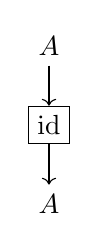
\begin{tikzpicture}
    \path
    (0,1) node(s) {$A$}
    (0,0) node[draw](id) {$\id$}
    (0,-1) node(t) {$A$}
    ;

    \draw[->] (s) -- (id);
    \draw[->] (id) -- (t);
  \end{tikzpicture}
  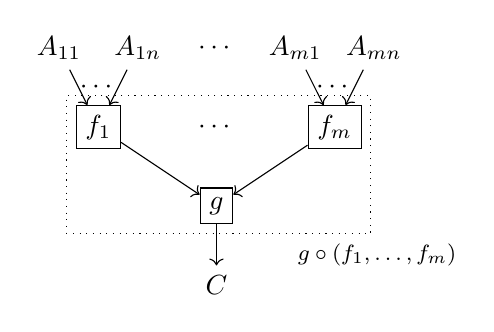
\begin{tikzpicture}
    \path
    (-2,2) node(A11) {$A_{11}$}
    (-1.5,1.5) node(A1dots) {$\cdots$}
    (-1,2) node(A1n) {$A_{1n}$}
    (0,2) node(Adots) {$\cdots$}
    (1,2) node(Am1) {$A_{m1}$}
    (1.5,1.5) node(Amdots) {$\cdots$}
    (2,2) node(Amn) {$A_{mn}$}

    (-1.5,1) node[draw](f1) {$f_1$}
    (0,1) node(fdots) {$\cdots$}
    (1.5,1) node[draw](fm) {$f_m$}

    (0,0) node[draw](g) {$g$}

    (0,-1) node(C) {$C$}
    ;

    \node[draw,dotted,fit=(f1) (fm) (g),
    label=below right:{\footnotesize$g \circ (f_1, \ldots, f_m)$}] (box) {};

    \draw[->] (A11) -- (f1);
    \draw[->] (A1n) -- (f1);
    \draw[->] (Am1) -- (fm);
    \draw[->] (Amn) -- (fm);
    \draw[->] (f1) -- (g);
    \draw[->] (fm) -- (g);
    \draw[->] (g) -- (C);
  \end{tikzpicture}

  \begin{displaymath}
    \begin{matrix}
      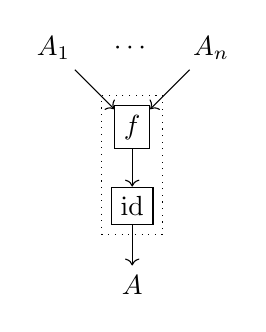
\begin{tikzpicture}[baseline]
        \path
        (-1,2) node(A1) {$A_1$}
        (0,2) node(Adots) {$\cdots$}
        (1,2) node(An) {$A_n$}
        (0,1) node[draw](f) {$f$}
        (0,0) node[draw](id) {$\id$}
        (0,-1) node(t) {$A$}
        ;

        \node[draw,dotted,fit=(f) (id)] {};

        \draw[->] (A1) -- (f);
        \draw[->] (An) -- (f);
        \draw[->] (f) -- (id);
        \draw[->] (id) -- (t);
      \end{tikzpicture}
      =
      \begin{tikzpicture}[baseline]
        \path
        (-1,1) node(A1) {$A_1$}
        (0,1) node(Adots) {$\cdots$}
        (1,1) node(An) {$A_n$}
        (0,0) node[draw](f) {$f$}
        (0,-1) node(t) {$A$}
        ;

        \draw[->] (A1) -- (f);
        \draw[->] (An) -- (f);
        \draw[->] (f) -- (t);
      \end{tikzpicture}
      &\phantom{mmmm}&
      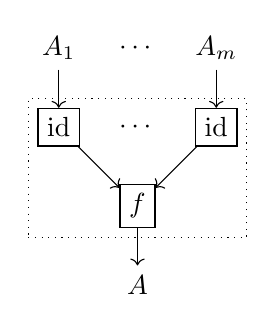
\begin{tikzpicture}[baseline]
        \path
        (-1,2) node(A1) {$A_1$}
        (0,2) node(Adots) {$\cdots$}
        (1,2) node(Am) {$A_m$}
        (-1,1) node[draw](id1) {$\id$}
        (0,1) node(iddots) {$\cdots$}
        (1,1) node[draw](idm) {$\id$}
        (0,0) node[draw](f) {$f$}
        (0,-1) node(t) {$A$}
        ;

        \node[draw,dotted,fit=(id1) (idm) (f)] {};

        \draw[->] (A1) -- (id1);
        \draw[->] (Am) -- (idm);
        \draw[->] (id1) -- (f);
        \draw[->] (idm) -- (f);
        \draw[->] (f) -- (t);
      \end{tikzpicture}
      =
      \begin{tikzpicture}[baseline]
        \path
        (-1,1) node(A1) {$A_1$}
        (0,1) node(Adots) {$\cdots$}
        (1,1) node(An) {$A_n$}
        (0,0) node[draw](f) {$f$}
        (0,-1) node(t) {$A$}
        ;

        \draw[->] (A1) -- (f);
        \draw[->] (An) -- (f);
        \draw[->] (f) -- (t);
      \end{tikzpicture}
    \end{matrix}
  \end{displaymath}

  \begin{displaymath}
    \begin{matrix}
      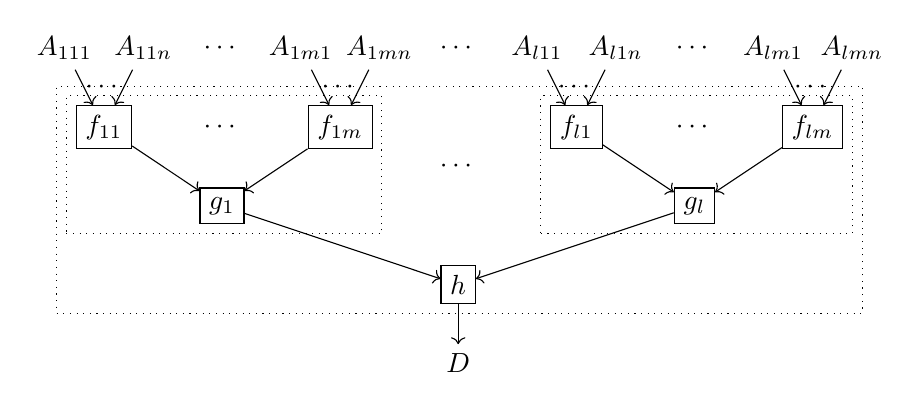
\begin{tikzpicture}
        \path
        % left
        (-5,2) node(A111) {$A_{111}$}
        (-4.5,1.5) node(A1dots) {$\cdots$}
        (-4,2) node(A11n) {$A_{11n}$}
        (-3,2) node(Adots) {$\cdots$}
        (-2,2) node(A1m1) {$A_{1m1}$}
        (-1.5,1.5) node(Amdots) {$\cdots$}
        (-1,2) node(A1mn) {$A_{1mn}$}

        (-4.5,1) node[draw](f11) {$f_{11}$}
        (-3,1) node(fdots) {$\cdots$}
        (-1.5,1) node[draw](f1m) {$f_{1m}$}

        (-3,0) node[draw](g1) {$g_1$}

        % right
        (1,2) node(Al11) {$A_{l11}$}
        (1.5,1.5) node(A1dots) {$\cdots$}
        (2,2) node(Al1n) {$A_{l1n}$}
        (3,2) node(Adots) {$\cdots$}
        (4,2) node(Alm1) {$A_{lm1}$}
        (4.5,1.5) node(Amdots) {$\cdots$}
        (5,2) node(Almn) {$A_{lmn}$}

        (1.5,1) node[draw](fl1) {$f_{l1}$}
        (3,1) node(fdots) {$\cdots$}
        (4.5,1) node[draw](flm) {$f_{lm}$}

        (3,0) node[draw](gl) {$g_l$}

        % middle
        (0,2) node {$\cdots$}
        (0,0.5) node {$\cdots$}
        (0,-1) node[draw](h) {$h$}
        (0,-2) node(D) {$D$}
        ;

        \node[draw,dotted,fit=(f11) (f1m) (g1)] (box1) {};
        \node[draw,dotted,fit=(fl1) (flm) (gl)] (boxl) {};
        \node[draw,dotted,fit=(box1) (boxl) (h)] (box) {};

        \draw[->] (A111) -- (f11);
        \draw[->] (A11n) -- (f11);
        \draw[->] (A1m1) -- (f1m);
        \draw[->] (A1mn) -- (f1m);
        \draw[->] (f11) -- (g1);
        \draw[->] (f1m) -- (g1);
        \draw[->] (g1) -- (h);

        \draw[->] (Al11) -- (fl1);
        \draw[->] (Al1n) -- (fl1);
        \draw[->] (Alm1) -- (flm);
        \draw[->] (Almn) -- (flm);
        \draw[->] (fl1) -- (gl);
        \draw[->] (flm) -- (gl);
        \draw[->] (gl) -- (h);

        \draw[->] (h) -- (D);
      \end{tikzpicture}
      \\=\\
      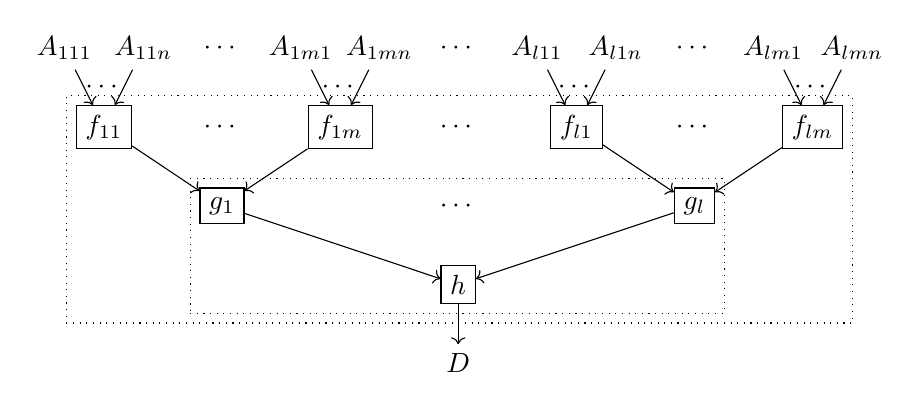
\begin{tikzpicture}
        \path
        % left
        (-5,2) node(A111) {$A_{111}$}
        (-4.5,1.5) node(A1dots) {$\cdots$}
        (-4,2) node(A11n) {$A_{11n}$}
        (-3,2) node(Adots) {$\cdots$}
        (-2,2) node(A1m1) {$A_{1m1}$}
        (-1.5,1.5) node(Amdots) {$\cdots$}
        (-1,2) node(A1mn) {$A_{1mn}$}

        (-4.5,1) node[draw](f11) {$f_{11}$}
        (-3,1) node(fdots) {$\cdots$}
        (-1.5,1) node[draw](f1m) {$f_{1m}$}

        (-3,0) node[draw](g1) {$g_1$}

        % right
        (1,2) node(Al11) {$A_{l11}$}
        (1.5,1.5) node(A1dots) {$\cdots$}
        (2,2) node(Al1n) {$A_{l1n}$}
        (3,2) node(Adots) {$\cdots$}
        (4,2) node(Alm1) {$A_{lm1}$}
        (4.5,1.5) node(Amdots) {$\cdots$}
        (5,2) node(Almn) {$A_{lmn}$}

        (1.5,1) node[draw](fl1) {$f_{l1}$}
        (3,1) node(fdots) {$\cdots$}
        (4.5,1) node[draw](flm) {$f_{lm}$}

        (3,0) node[draw](gl) {$g_l$}

        % middle
        (0,2) node {$\cdots$}
        (0,1) node {$\cdots$}
        (0,0) node {$\cdots$}
        (0,-1) node[draw](h) {$h$}
        (0,-2) node(D) {$D$}
        ;

        \node[draw,dotted,fit=(g1) (gl) (h)] (boxi) {};
        \node[draw,dotted,fit=(f11) (f1m) (fl1) (flm) (boxi)] (boxo) {};

        \draw[->] (A111) -- (f11);
        \draw[->] (A11n) -- (f11);
        \draw[->] (A1m1) -- (f1m);
        \draw[->] (A1mn) -- (f1m);
        \draw[->] (f11) -- (g1);
        \draw[->] (f1m) -- (g1);
        \draw[->] (g1) -- (h);

        \draw[->] (Al11) -- (fl1);
        \draw[->] (Al1n) -- (fl1);
        \draw[->] (Alm1) -- (flm);
        \draw[->] (Almn) -- (flm);
        \draw[->] (fl1) -- (gl);
        \draw[->] (flm) -- (gl);
        \draw[->] (gl) -- (h);

        \draw[->] (h) -- (D);
      \end{tikzpicture}
    \end{matrix}
  \end{displaymath}
\end{definition}

Multicategories have been used as a framework for reasoning with multilinear
maps in linear algebra. \todo{Reference?}
We can produce a multicategory where the objects are vector spaces, and the
multimorphisms are multilinear maps.
In this setting, we can give a universal property to the tensor product of
vector spaces.

\begin{definition}[tensor product \& tensor unit]
  Given a multicategory $\C$, a \emph{tensor product} in $\C$ is a function
  ${\otimes} : \obj\C \times \obj\C \to \obj\C$ and for each pair of objects
  $A$ and $B$, a multimorphism ${\otimes} : A, B \to A \otimes B$ such that,
  for any multimorphism $f : A, B \to C$, there is a unique way to factor $f$
  through $\otimes$, as shown below.
  Similarly, a \emph{tensor unit} is an object $I$ of $\C$ and a multimorphism
  $I : \varepsilon \to I$ supporting a nullary unique factorisation.

  \begin{tikzcd}
    A, B \arrow[rd,"f"'] \arrow[r,"\otimes"] & A \otimes B \arrow[d, dashed] \\
    & C
  \end{tikzcd}
  \begin{tikzcd}
    \varepsilon \arrow[rd,"f"'] \arrow[r,"I"] & I \arrow[d, dashed] \\
    & C
  \end{tikzcd}
\end{definition}

As the proliferation of ellipses suggests, the definition of
\emph{multicategory} I gave above is not entirely rigorous.
Indeed, mechanising the multicategory definition in a reasonably usable way is
considered an open problem. \todo{Check that no-one has done it}
However, we \emph{can} achieve a simple and usable definition in the special
case of \emph{Cartesian} multicategories.

Ordinary multicategories are to monoidal categories as Cartesian multicategories
are to Cartesian categories (i.e., categories with all finite products).
Cartesian multicategories can be defined in terms of ordinary multicategories
--- they are multicategories satisfying the usual ``structural rules'' below
and satisfying various coherence conditions on them.

\begin{align*}
  e &: \hom(\Gamma, A, B, \Delta; C) \to \hom(\Gamma, B, A, \Delta; C) \\
  w &: \hom(\Gamma; B) \to \hom(\Gamma, A; B) \\
  c &: \hom(\Gamma, A, A; B) \to \hom(\Gamma, A; B)
\end{align*}

However, we can bypass ordinary multicategories entirely, and give the following
definition inspired by our earlier formulation of intuitionistic logic.
I define Cartesian multicategories in tandem with the category of contexts and
substitutions that a Cartesian multicategory yields.

\begin{definition}
  A \emph{Cartesian multicategory} comprises the following.

  \begin{itemize}
    \item We have a collection of objects $\obj$.
          We call a list of objects a \emph{context}.
    \item For each context $\Gamma$ and object $A$, we have a set of
          (multi)morphisms $\hom(\Gamma; A)$.
          From this, we derive, for any contexts $\Gamma$ and $\Delta$, a set
          of \emph{substitutions}
          $\sub(\Gamma; \Delta) \coloneqq \prod X \in \Delta.~\hom(\Gamma; X)$.
    \item For every $i : A \in \Gamma$, we have an identity morphism
          $\id(i) : \hom(\Gamma; A)$.
          The collection of identity morphisms over $\Gamma$ serves as the
          identity substitution $\id^s : \sub(\Gamma; \Gamma)$.
    \item For substitution $\sigma : \sub(\Gamma; \Delta)$ and morphism
          $f : \hom(\Delta; A)$, we get a composite morphism
          $\sigma ; f : \hom(\Gamma; A)$.
          This allows us to compose substitutions; for
          $\sigma : \sub(\Gamma; \Delta)$ and $\tau : \sub(\Delta; \Theta)$,
          let $\sigma;^s \tau \coloneqq \lambda k.~\sigma; \tau(k)$.
    \item Identity and composition satisfy the following laws.
          \begin{itemize}
            \item $\sigma; \id(i) = \sigma(i)$
            \item $\id^s; f = f$
            \item $(\sigma;^s \tau); f = \sigma; (\tau; f)$
          \end{itemize}
          It is a simple exercise to see that these laws exactly give us the
          category laws of identity and associativity for substitutions.
  \end{itemize}
\end{definition}

The category of contexts and substitutions is furthermore Cartesian, with the
product being given by context concatenation.

\section{Weighted multicategories}
Where Cartesian multicategories give semantics to simply typed
$\lambda$-calculus, we want to find a kind of multicategories that give
semantics to $\name$.

\section{Applications}

\chapter{Semantics in worldly relations}\label{sec:wrel}

\def\prefix{../generic-lr/src/latex}

\CatchFileBetweenTags{\exItypes}%
{\prefix/Generic/Linear/Example/PaperExamples.tex}{exItypes}
\CatchFileBetweenTags{\exIlabels}%
{\prefix/Generic/Linear/Example/PaperExamples.tex}{exIlabels}
\CatchFileBetweenTags{\exIfunrules}%
{\prefix/Generic/Linear/Example/PaperExamples.tex}{exIfunrules}
\CatchFileBetweenTags{\exIsumrules}%
{\prefix/Generic/Linear/Example/PaperExamples.tex}{exIsumrules}

\CatchFileBetweenTags{\Premises}%
{\prefix/Generic/Linear/Syntax.tex}{Premises}
\CatchFileBetweenTags{\Rule}%
{\prefix/Generic/Linear/Syntax.tex}{Rule}
\CatchFileBetweenTags{\System}%
{\prefix/Generic/Linear/Syntax.tex}{System}

\CatchFileBetweenTags{\semp}%
{\prefix/Generic/Linear/Syntax/Interpretation.tex}{semp}
\CatchFileBetweenTags{\semr}%
{\prefix/Generic/Linear/Syntax/Interpretation.tex}{semr}
\CatchFileBetweenTags{\sems}%
{\prefix/Generic/Linear/Syntax/Interpretation.tex}{sems}

\CatchFileBetweenTags{\SimplePremises}%
{\prefix/Generic/Simple/Syntax.tex}{SimplePremises}

\section{Building up}

We assume that a type system comprises a set of (unparametrised) rules, each
of which has a conclusion and several premises containing subterms.
The primary investigation of this work is into what form the premises can take
while maintaining useful features of syntax.
We shall start with simple forms, allowing just for multiple subterms, and
then build on resource-sensitive bunches, variable binding, and modalities.

\System{}
\Rule{}

Given some way \AgdaFunction{⟦\AgdaUnderscore{}⟧p} of interpreting
\AgdaDatatype{Premises} in a \AgdaRecord{Ctx}, we can interpret a
\AgdaDatatype{Rule} against a conclusion and a context by checking that its
stated conclusion matches and then interpreting its premises.
Then, the entire \AgdaDatatype{System} can be interpreted by picking a rule
label (including parameters) \AgdaBound{l} and interpreting the selected rule
\AgdaBound{rs}\AgdaSpace{}\AgdaBound{l}.

\semr{}
\sems{}

\subsection{The language of Cartesian products}

\SimplePremises

\section{Bunched functions}

Suppose we have a left $R$-semimodule $M$.
Then we can define the following connectives on indexed type families.

\begin{align*}
  \top~z &:= \top \\
  (P \wedge Q)~z &:= P~z \wedge Q~z \\
  (P \to Q)~z &:= P~z \to Q~z \\
  I~z &:= z \subres 0 \\
  (P * Q)~z &:= \exists x,y.~z \subres x+y \wedge P~x \wedge Q~y \\
  (P \wand Q)~y &:= \forall x,z.~z \subres x+y \to P~x \to Q~z \\
  (r \cdot P)~z &:= \exists x.~z \subres rx \wedge P~x
\end{align*}

\paragraph{Agda definitions}
To follow.

The first six of these connectives are somewhat standard, the first three
corresponding to the usual sharing connectives and the second three
corresponding to the usual separating connectives.
The final connective, $r \cdot P$, is new.
We choose $\exists$ rather than $\forall$ because scaling will usually occur in
premises, i.e., to the left of arrows, and we want to avoid anything
higher-order.

\section{Generic syntax}

Rules $R$, premises $P$ and $Q$.

\begin{align*}
  R &::= P/A \\
  P,Q &::= \grR\Theta \vdash A \mid \top \mid P \wedge Q \mid I \mid P * Q
        \mid \gr r \cdot P
\end{align*}

Example rules:

\begin{itemize}
  \item With-introduction: ${\vdash A} \wedge {\vdash B} / A \with B$
  \item Annotated arrow introduction:
    ${\gr rA \vdash B} / \gr rA \multimap B$
  \item Annotated arrow elimination:
    ${\vdash \gr rA \multimap B} * \gr r \cdot {\vdash A} / B$
  \item Cases of annotated sum:
    ${\vdash \gr rA \oplus \gr sB}
    * ({\gr rA \vdash C} \wedge {\gr sB \vdash C}) / C$
\end{itemize}

\paragraph{Agda example}

We start by defining our types \AgdaDatatype{Ty}, which in this case will be the
conclusions of our judgements.
\AgdaFunction{Ann} is the type of usage annotations, which for now is an
arbitrary skew semiring.
We also have a type of rule labels \AgdaDatatype{`Sys}, which specifies all of
the parameters of a typing rule except for its conclusion and premises.
For example, in the \AgdaInductiveConstructor{`case} label, we need to fill in
the two summands (types \AgdaBound{A} and \AgdaBound{B}), as well as the return
type \AgdaBound{C}.
The actual form of the rule will be specified later.

\exItypes{} \exIlabels{}

We are then ready to build a system \AgdaFunction{Sys} with conclusions
\AgdaDatatype{Ty}, usage annotations \AgdaFunction{Ann}, and labels
\AgdaDatatype{`Sys}.
The rule corresponding to each label is given in the following.

The \AgdaInductiveConstructor{`lam} rule has one premise, which binds one
variable with usage annotation \AgdaBound{r} and type \AgdaBound{A}.
The \AgdaInductiveConstructor{`app} rule has two premises combined with
separating conjunction.
Furthermore, the second premise (corresponding to the argument of the function)
is subject to scaling by \AgdaBound{r}.
Intuitively, this description means that we must have enough of each variable to
use some in building a function, and then use some more \AgdaBound{r} times to
build enough arguments.

\exIfunrules{}

In the rules for sums, we use an alternative notation for rule descriptions,
with \AgdaFunction{{---}{---}} being an infix version of
\AgdaInductiveConstructor{rule}.
The introduction rules \AgdaInductiveConstructor{`inl} and
\AgdaInductiveConstructor{`inr} are straightforward --- each has one
premise which binds no new variables.
The \AgdaInductiveConstructor{`case} rule is more complicated.
The premises are first split into the eliminand and the continuations, using the
separating conjunction we saw for \AgdaInductiveConstructor{`app}.
However, the continuations are connected via the sharing conjunction, reflecting
the fact that in any given run of the program, only one of the branches will be
taken, so usages from each individually should be added to usages of the
eliminand.

\exIsumrules{}

\paragraph{Interpretation as syntax}
We can say something like ``premise connectives are interpreted as the
corresponding bunched connectives, where appropriate''.

\begin{align*}
  \sem{P/A} &:= \sem P \to {- \vdash A} \\
  \sem{\grR\Theta \vdash A} &:= {-, \grR\Theta \vdash A} \\
  \sem{\top} &:= \top \\
  \sem{P \wedge Q} &:= \sem P \wedge \sem Q \\
  \sem{I} &:= I \\
  \sem{P * Q} &:= \sem P * \sem Q \\
  &\ldots
\end{align*}

\paragraph{Agda version}
The interpretation of a system is the selection of a rule, together with the
interpretation of that rule.

\sems{}

The interpretation of a rule is a check that the rule targets the desired
conclusion, together with the interpretation of the rules premises.

\semr{}

For the premises, connectives are interpreted in the obvious way.
Premises can ask for subterms via the $\AgdaInductiveConstructor{\_`⊢\_}$
constructor, which supplies the new variables (in particular, each variable's
type and usage annotation) \AgdaBound{Γ} and the desired conclusion
\AgdaBound{A} of the subterm.

\semp{}

\section{Values and computations}

Following \cite{AACMM20}, we call any semantic realisation of a variable a
\emph{value}, and any semantic realisation of a term a \emph{computation}.
Scoped families of values are named $\mathcal V$, while scoped families of
computations are named $\mathcal C$.
\todo{This wording is difficult.}
Values and computations are concepts with attitudes.

\section{Environments}

An environment is a linear map from variables in one context to values in
another.

\missingfigure{Agda definition of \AgdaRecord{\_{---}Env}}

An environment in \AgdaBound{PΓ} for \AgdaBound{$\mathcal V$}-values in
\AgdaBound{QΔ} is a linear map \AgdaField{M} such that $Q \le PM$ and for any
$P'$ and $Q'$ such that $Q' \le P'M$, a function from variables in $P'Γ$ to
\AgdaBound{$\mathcal V$}-values in $Q'Δ$.

\section{Thinnings}

\todo[inline]{I think thinnings should be called \emph{renamings}.}

In a usage-annotated sequent calculus, their are 4 basic structural rules:
exchange, weakening of $0$-annotated formulae, contraction of $+$-annotated
formulae, and subusaging.
Their typical forms are given below.

\begin{mathpar}
  \inferrule*[right=exch]
  {\grP\Gamma, \gr sB, \gr rA, \grQ\Delta \vdash Z}
  {\grP\Gamma, \gr rA, \gr sB, \grQ\Delta \vdash Z}
  \and
  \inferrule*[right=weak]
  {\grP\Gamma, \grQ\Delta \vdash Z}
  {\grP\Gamma, 0A, \grQ\Delta \vdash Z}
  \and
  \inferrule*[right=cont]
  {\grP\Gamma, \gr rA, \gr sA, \grQ\Delta \vdash Z}
  {\grP\Gamma, (\gr r + \gr s)A, \grQ\Delta \vdash Z}
  \and
  \inferrule*[right=subuse]
  {\grP \le \grQ \\\\ \grQ\Gamma \vdash Z}
  {\grP\Gamma \vdash Z}
\end{mathpar}

Generalising away from $\vdash$, it can be helpful to know when an arbitrary
scoped family respects these structural rules.
First, we note that the structural rules of sequent calculus correspond
directly to \emph{renaming} in natural deduction.
A renaming is an environment of variables, i.e., a \emph{linear} map from
variables to variables.
The linearity is what gives us the restrictions on annotations in the weakening
and contraction rules.

\missingfigure{Example renaming}

%A thinning is an environment of syntactic variables.
%In effect, thinning allows for permutation and slackening of existing
%variables, and introduction of new discardable variables at any position.
%These actions are in direct correspondence with the usual sequent calculus
%structural rules of exchange, contraction, and weakening, as well as subusaging.

Given this definition, $\square$ and \texttt{Thinnable} are as in AACMM.
\texttt{Kripke} is modified to use separating implication.

\section{Substitution}

\todo[inline]{This seems like a good place to introduce substitution, straight
after renaming, though we don't even have terms yet.}
Whereas a renaming is a linear map from variables to variables, a substitution
is a linear map from variables to terms.

\section{A layer of syntax is functorial}

\chapter{Applications}\label{sec:applications}

\section{Usage checker}\label{sec:usage-checker}
\section{Linear/non-linear logic}\label{sec:lnl}
We can express Benton's linear/non-linear logic~\cite{Benton94} in the
framework.
There are two apparent discrepancies between L/nL and what we have seen so far
to be expressible in the framework: the existence of multiple judgement modes
and the restriction on the kinds of assumptions based on the mode.
We will start by addressing these discrepancies, before presenting the encoding
in full and proving the resulting system logically equivalent to
$\lambda\gr{\mathcal R}$.

\subsection{Encoding L/nL}

In L/nL, we have a \emph{linear} and an \emph{intuitionistic} mode, with
separate types (respectively $A$ and $X$) and typing judgements (respectively
$\vdash_{\mathcal L}$ and $\vdash_{\mathcal C}$) connected by modalities $F$ and
$G$.
The mode of the conclusion type is the same as the mode of the judgement, so
only a distinction in the conclusion mode is necessary.
To achieve this distinction in the types, I have an indexed type family
$\mathrm{Ty} : \mathrm{Frag} \to \mathrm{Set}$, and set the framework types to
be the type $(f : \mathrm{Frag}) \times \mathrm{Ty}\,f$.
% \AgdaDatatype{Ty}\AgdaSymbol{:}\AgdaDatatype{Frag}\AgdaSymbol{$\to$}
% \AgdaDatatype{Set}
I present these judgements in a standard paper style in \cref{fig:lnl-types}.

In L/nL, while linear judgements can have both linear and intuitionistic
assumptions, intuitionistic judgements can only have intuitionistic assumptions.
I encode this invariant on intuitionistic judgements using the $\Box$
premise combinator on all intuitionistic conclusions and wherever
intuitionistic premises occur for linear conclusions, as seen in
\cref{fig:lnl-desc}.
This scheme means that the rules contain the maximal number of boxes, which is
convenient when consuming terms.
For ease of \emph{producing} terms, we would want a ``garbage in; garbage out''
style with a minimal number of boxes, which could be achieved in two different
ways:
\begin{itemize}
  \item Ensure that $\Gamma, \gr1\,\lin A \vdash \intu X$ is never derivable.
    This leaves boxes only on rules $1$-I and $G$-I.
  \item Ensure that, when working bottom-up, we never transition from a linear
    to an intuitionistic conclusion with linear assumptions present.
    This leaves boxes only on rules $F$-I and $G$-E.
\end{itemize}
It would be interesting to show the equivalence of these three approaches, but
that is left to future work.

\begin{figure}
  \begin{align*}
    A, B, C &\Coloneqq I \mid A \otimes B \mid A \multimap B \mid FX \\
    X, Y, Z &\Coloneqq 1 \mid X \times Y \mid X \to Y \mid GA \\
    \mathcal J &\Coloneqq \lin A \mid \intu X
  \end{align*}
  \caption{Types and judgement forms of L/nL}
  \label{fig:lnl-types}
\end{figure}

\begin{figure}
  \begin{mathpar}
    % lin rules
    \ebrule[comb]{%
      \hypo{I^*}
      \infer1[$I$-I]{\vdash \lin I}
    }
    \and
    \ebrule[comb]{%
      \hypo{\vdash \lin I}
      \hypo{*}
      \hypo{\vdash \lin C}
      \infer3[$I$-E]{\vdash \lin C}
    }
    \and
    \ebrule[comb]{%
      \hypo{\vdash \lin A}
      \hypo{*}
      \hypo{\vdash \lin B}
      \infer3[$\otimes$-I]{\vdash \lin A \otimes B}
    }
    \and
    \ebrule[comb]{%
      \hypo{\vdash \lin A \otimes B}
      \hypo{*}
      \hypo{\gr1\,\lin A, \gr1\,\lin B \vdash \lin C}
      \infer3[$\otimes$-E]{\vdash \lin C}
    }
    \and
    \ebrule[comb]{%
      \hypo{\gr1\,\lin A \vdash \lin B}
      \infer1[$\multimap$-I]{\vdash \lin A \multimap B}
    }
    \and
    \ebrule[comb]{%
      \hypo{\vdash \lin A \multimap B}
      \hypo{*}
      \hypo{\vdash \lin A}
      \infer3[$\multimap$-E]{\vdash \lin B}
    }
    \and
    \ebrule[comb]{%
      \hypo{\Box\plr{\vdash \intu X}}
      \infer1[$F$-I]{\vdash \lin FX}
    }
    \and
    \ebrule[comb]{%
      \hypo{\vdash \lin FX}
      \hypo{*}
      \hypo{\gr\omega\,\intu X \vdash \lin C}
      \infer3[$F$-E]{\vdash \lin C}
    }
    \and
    % int rules
    \ebrule[comb]{%
      \hypo{\Box\plr{\dot1}}
      \infer1[$1$-I]{\vdash \intu 1}
    }
    \and
    \text{(no $1$-E)}
    \and
    \ebrule[comb]{%
      \hypo{\Box(\vdash \intu X}
      \hypo{\dottimes}
      \hypo{\vdash \intu Y)}
      \infer3[$\times$-I]{\vdash \intu X \times Y}
    }
    \and
    \ebrule[comb]{%
      \hypo{\Box\plr{\vdash \intu X \times Y}}
      \infer1[$\times$-El]{\vdash \intu X}
    }
    \and
    \ebrule[comb]{%
      \hypo{\Box\plr{\vdash \intu X \times Y}}
      \infer1[$\times$-Er]{\vdash \intu Y}
    }
    \and
    \ebrule[comb]{%
      \hypo{\Box\plr{\gr\omega\,\intu A \vdash \intu B}}
      \infer1[$\to$-I]{\vdash \intu A \to B}
    }
    \and
    \ebrule[comb]{%
      \hypo{\Box(\vdash \intu A \to B}
      \hypo{\dottimes}
      \hypo{\vdash \intu A)}
      \infer3[$\to$-E]{\vdash \intu B}
    }
    \and
    \ebrule[comb]{%
      \hypo{\Box\plr{\vdash \lin A}}
      \infer1[$G$-I]{\vdash \intu GA}
    }
    \and
    \ebrule[comb]{%
      \hypo{\Box\plr{\vdash \intu GA}}
      \infer1[$G$-E]{\vdash \lin A}
    }
  \end{mathpar}
  \caption{Description of the logical rules of L/nL}
  \label{fig:lnl-desc}
\end{figure}

\begin{proposition}
  We can construct the following translations.
  \begin{align}
    (\Theta \vdash_{\mathcal C} X) &\to (\gr\omega\Theta \vdash \intu X) \\
    (\Theta; \Gamma \vdash_{\mathcal L} A) &\to
    (\gr\omega\Theta, \gr1\Gamma \vdash \lin A)
  \end{align}
\end{proposition}

\begin{proposition}
  We can construct the following translations, where $\Gamma_{\gr r}$ is the
  list of types in $\Gamma$ that are annotated $\gr r$.%
  \todo{I'm not sure the resultant contexts are well formed.}
  \begin{align}
    (\Gamma \vdash \intu X) &\to (\Gamma_{\gr\omega} \vdash_{\mathcal C} X) \\
    (\Gamma \vdash \lin A) &\to
    (\Gamma_{\gr\omega}; \Gamma_{\gr1} \vdash_{\mathcal L} A)
  \end{align}
\end{proposition}

\subsection{Translating between L/nL and $\lambda\gr{\mathcal R}$}

The translations largely follow Benton's originals.
In this section, I take $\name$ to be the system described in
\cref{fig:lr-bunched} instantiated to the $\{\gr0 > \gr\omega < \gr1\}$
posemiring and restricted to the fragment with only connectives $I$, $\otimes$,
$\multimap$, and $\oc\gr\omega$.
Notably, this excludes $\oc\gr0$ and $\oc\gr1$.
I write $\oc\gr\omega$ as just $\oc$, as in traditional linear logic.
Under these restrictions, Benton's translations of types can be used verbatim
(\cref{fig:lnl-lr-types}).

\begin{figure}
  \centering
  \begin{subfigure}{.49\linewidth}
    \centering
    \begin{align*}
      (-)^\circ : \mathrm{Ty}_{\name} \to \mathrm{Ty}_{\lin} \\
      \begin{aligned}
        I^\circ &= I \\
        \plr{A \otimes B}^\circ &= A^\circ \otimes B^\circ \\
        \plr{A \multimap B}^\circ &= A^\circ \multimap B^\circ \\
        \plr{\oc A}^\circ &= GFA^\circ
      \end{aligned}
    \end{align*}
  \end{subfigure}
  \begin{subfigure}{.49\linewidth}
    \centering
    \begin{align*}
      (-)^* : \mathrm{Ty}_\lnl \to \mathrm{Ty}_{\name} \\
      \begin{aligned}
        I^* &= I \\
        \plr{A \otimes B}^* &= A^* \otimes B^* \\
        \plr{A \multimap B}^* &= A^* \multimap B^* \\
        \plr{FX}^* &= \oc X^* \\
        1^* &= I \\
        \plr{X \times Y}^* &= \oc X^* \otimes \oc Y^* \\
        \plr{X \to Y}^* &= \oc X^* \multimap Y^* \\
        \plr{GA}^* &= A^*
      \end{aligned}
    \end{align*}
  \end{subfigure}
  \caption{Translation of types between L/nL and $\name$}
  \label{fig:lnl-lr-types}
\end{figure}

We extend both $(-)^\circ$ and $(-)^*$ to contexts pointwise on the types.
For $(-)^\circ$, this means that the translation lands outside what is usually
expressible in L/nL whenever the context contains annotation $\gr\omega$.
For example, $\plr{\gr\omega I}^\circ = \plr{\gr\omega\,\lin I}$, and we do not
see ``$\gr\omega\,\lin$'' in translations from Benton's L/nL.
This could be fixed by inserting $G$ in such cases.
As for $(-)^*$, note that we do not insert a $\oc$ on intuitionistic assumptions
as Benton does.
Instead, the annotation $\gr\omega$ achieves the same effect for us.
This discrepancy essentially amounts to the fact that $\name$ is more like DILL
than Girard's ILL, and Benton's translations act upon the latter.

\begin{theorem}
  We can translate from $\name$ to the linear fragment of L/nL.
  \begin{align}
    (\Gamma \vdash_{\name} A) \to (\Gamma^\circ \vdash_\lnl \lin A^\circ)
  \end{align}
\end{theorem}

\begin{theorem}
  We can translate any L/nL term to a $\name$ term as follows.
  \begin{align}
    (\Gamma \vdash_\lnl \intu X) &\to (\Gamma^* \vdash_{\name} X^*) \\
    (\Gamma \vdash_\lnl \lin A) &\to (\Gamma^* \vdash_{\name} A^*)
  \end{align}
\end{theorem}

\section{$\mu\tilde\mu$-calculus}\label{sec:mmt}
\section{Graphs}\label{sec:graphs}

\chapter{Conclusions}\label{sec:conc}

FIXME: this chapter is directly from the ESOP22 paper.

We have presented a framework for doing metatheory for a class of substructural
type systems in Agda.
The framework gives us renaming, substitution, and a usage elaborator for new
syntaxes for free, which we hope can facilitate prototyping and the
mechanisation of more interesting semantic results.
Beside the mechanised framework itself, we believe its methodology --- the use
of bunched premise combinators --- can guide and simplify the development of
(potentially unmechanised) substructural type systems.

Our account of substructurality is based on the linear algebraic
principles described by \citet{WA21}.
However, these details only really affect the definition of environment,
in which the use of linear maps is motivated by them being the standard notion
of morphism between vectors.
We could imagine that a similar notion of morphism is found for the kind of
annotations found in \citet{LicataSR17}, allowing a framework to consider
finer substructural systems.



%%%%%%%%%%%%%%%%%%%%%%%%%%%%%%%%%%%%%%%%%%%%%%%%%%%%%%%%%%%%%%
\appendix
\chapter{Stuff That Didn't Fit Anywhere Else}
%%%%%%%%%%%%%%%%%%%%%%%%%%%%%%%%%%%%%%%%%%%%%%%%%%%%%%%%%%%%%%


%%%%%%%%%%%%%%%%%%%%%%%%%%%%%%%%%%%%%%%%%%%%%%%%%%%%%%%%%%%%%%
\addcontentsline{toc}{chapter}{Bibliography}
\bibliographystyle{alpha}
\bibliography{quantitative}

\end{document}
